
%%==================================================
%% Ma Thesis.tex for DUT Thesis
%% version: 1.2
%% last update: Apr 27th, 2022
%%==================================================


\documentclass[twoside,doctor,hide]{DUT-thesis-grd}

% 需要删除
% 自定义宏
\def\todo{\textcolor{red}{TODO}}
% END 

% 自己额外导入的包
\usepackage{ulem}
% If you comment hyperref and then uncomment it, you should delete
% egpaper.aux before re-running latex.  (Or just hit 'q' on the first latex
% run, let it finish, and you should be clear).
%\usepackage[pagebackref=true,breaklinks=true,letterpaper=true,colorlinks,bookmarks=false]{hyperref}
%
%\usepackage[colorlinks,
%linkcolor=red,
%anchorcolor=blue,
%citecolor=green
%]{hyperref}

%\usepackage[dvipdfm,  %pdflatex,pdftex这里决定运行文件的方式不同
%pdfstartview=FitH,
%CJKbookmarks=true,
%bookmarksnumbered=true,
%bookmarksopen=true,
%colorlinks, %注释掉此项则交叉引用为彩色边框(将colorlinks和pdfborder同时注释掉)
%pdfborder=001,   %注释掉此项则交叉引用为彩色边框
%linkcolor=green,
%anchorcolor=green,
%citecolor=green
%]{hyperref}  

\usepackage{hyperref} 
\hypersetup{
	colorlinks=true,
	citecolor=blue,
	linkcolor=red,
	urlcolor=green}


%\usepackage[colorlinks]{hyperref}
\usepackage{pifont}
\usepackage{color}
\usepackage{booktabs}
\usepackage{multirow}
\usepackage{color}
%\usepackage{subcaption}
%\usepackage{cite}
%\usepackage[numbers]{natbib}
\usepackage{soul}
% 针对\cite和\ref命令 (通常用下面两个)
%\soulregister\cite
%\soulregister\ref 
% 针对其他命令
%\soulregister\citep7 % 针对\citep命令
%\soulregister\citet7 % 针对\citet命令
%\soulregister\pageref7 % 针对\pageref命令

%==============更改数学字体设置,Latin Modern Math 默认的的确有点细,看个人需要,下面提供一种方法,需要的可以取消注释=========%

% \usepackage[bold-style=ISO]{unicode-math} %采用unicode-math,可以直接输入Unicode公式,当然传统的输入就行
% \setmathfont{XITS Math}  %目前unicode-math 支持几种数学字体,具体用法可以查看帮助文档,这里采用类似times字体科学数学字体,可以取消注释对比


\begin{document}

%%%%%%%%%%%%%%%%%%%%%%%%%%%%%%
%% 封面
%%%%%%%%%%%%%%%%%%%%%%%%%%%%%%

% 封面绘制
% \maketitle


% 论文原创性声明和使用授权
% \makeDeclareOriginal
%\addcontentsline{toc}{chapter}{大连理工大学学位论文版权使用授权书}


%%%%%%%%%%%%%%%%%%%%%%%%%%%%%%
%% 前置部分
%%%%%%%%%%%%%%%%%%%%%%%%%%%%%%
% \frontmatter

% 摘要
% %%==================================================
%% abstract.tex for DUT  Thesis
%% version: 0.1
%% last update: Apr 27th, 2022
%%==================================================

\begin{abstract}
大连理工大学硕士研究生撰写学位论文应当符合写作规范和排版格式的要求,以下格式为研究生院依据国家标准和行业规范所编制的硕士学位论文模板,供硕士研究生参照使用。\par 论文摘要是学位论文的缩影,文字要简练、明确。内容要包括目的、方法、结果和结论。单位制一律换算成国际标准计量单位制,除特殊情况外,数字一律用阿拉伯数码。文中不允许出现插图,重要的表格可以写入。\par  摘要的主要内容为,简述全文的目的和意义、采用方法、主要研究内容和结论。\par 篇幅以一页为限,摘要正文后列出3-5个关键词,关键词与摘要之间空一行。\par“关键词:”是关键词部分的引导,不可省略。\par 关键词请尽量用《汉语主题词表》等词表提供的规范词。关键词之间用分号间隔,末尾不加标点。


\keywords{写作规范;排版格式;硕士学位论文}
\end{abstract}

\begin{englishabstract}

Contents of the abstract.Times New Roman.
   
\englishkeywords{Write Criterion; Typeset Format; Master's Degree Thesis}

\end{englishabstract}

%% 符号对照表,可选,如不用可注释掉

% 加入目录
\tableofcontents

% \tableofengcontents

%加入图、表索引(同时取消图表索引中章之间的垂直间隔)
% \let\origaddvspace\addvspace
% \renewcommand{\addvspace}[1]{}
% \addcontentsline{toc}{chapter}{图目录}
% \listoffigures
% \addcontentsline{toc}{chapter}{表目录}
% \listoftables
% \renewcommand{\addvspace}[1]{\origaddvspace{#1}}


% \begin{denotation}
	\vspace{-20pt}
\begin{center}
% Table generated by Excel2LaTeX from sheet 'Sheet1'
\begin{table}[htbp]
	\centering
	\begin{tabular}{rrrcccccccccccccrrr}
		\toprule
		&       &       & \multicolumn{3}{c}{\textbf{符  号}} &       & \multicolumn{4}{c}{\textbf{代表意义}} &       & \multicolumn{4}{c}{\textbf{单位或定义}} &       &       &  \\
		&       &       & \multicolumn{3}{c}{\textbf{英文字母}} &       & \multicolumn{4}{c}{}          &       & \multicolumn{4}{c}{}          &       &       &  \\
		&       &       & \multicolumn{3}{c}{\textit{A}} &       & \multicolumn{4}{c}{加热面面积}     &       & \multicolumn{4}{c}{$\rm{cm^2}$}       &       &       &  \\
		&       &       & \multicolumn{3}{c}{$A_{\rm{liquid}}$} &       & \multicolumn{4}{c}{加热面润湿区域}   &       & \multicolumn{4}{c}{$\rm{cm^2}$}       &       &       &  \\
		&       &       & \multicolumn{3}{c}{\textit{B}} &       & \multicolumn{4}{c}{热流密度决定性偏差} &       & \multicolumn{4}{c}{\textbackslash{}} &       &       &  \\
		&       &       & \multicolumn{3}{c}{Cp} &       & \multicolumn{4}{c}{比热容}       &       & \multicolumn{4}{c}{kJ/(kg·K)} &       &       &  \\
		\multicolumn{4}{c}{}          &       &
		\multicolumn{4}{c}{}          &       & \multicolumn{4}{c}{}          &       &       &  \\
		&       &       & \multicolumn{3}{c}{\textbf{无量纲量}} &       & \multicolumn{4}{c}{}          &       & \multicolumn{4}{c}{}          &       &       &  \\
		&       &       & \multicolumn{3}{c}{\textit{Re}} &       & \multicolumn{4}{c}{雷诺数}       &       & \multicolumn{4}{c}{}          &       &       &  \\
		&       &       & \multicolumn{3}{c}{}  &       & \multicolumn{4}{c}{斯特劳哈尔数}    &       & \multicolumn{4}{c}{}          &       &       &  \\
		&       &       & \multicolumn{3}{c}{}  &       & \multicolumn{4}{c}{韦伯数}       &       & \multicolumn{4}{c}{}          &       &       &  \\
		&       &       & \multicolumn{3}{c}{}  &       & \multicolumn{4}{c}{}          &       & \multicolumn{4}{c}{}          &       &       &  \\
		&       &       & \multicolumn{3}{c}{\textbf{希腊字母}} &       & \multicolumn{4}{c}{}          &       & \multicolumn{4}{c}{}          &       &       &  \\
		&       &       & \multicolumn{3}{c}{}  &       & \multicolumn{4}{c}{密度}        &       & \multicolumn{4}{c}{$\rm{kg/{m}^{3}}$}     &       &       &  \\
		&       &       & \multicolumn{3}{c}{}  &       & \multicolumn{4}{c}{黏度}        &       & \multicolumn{4}{c}{Pa$\cdot$s}      &       &       &  \\
		&       &       & \multicolumn{3}{c}{}  &       & \multicolumn{4}{c}{蒸发效率}      &       & \multicolumn{4}{c}{}          &       &       &  \\
		&       &       & \multicolumn{3}{c}{}  &       & \multicolumn{4}{c}{}          &       & \multicolumn{4}{c}{}          &       &       &  \\
		&       &       & \multicolumn{3}{c}{\textbf{下标}} &       & \multicolumn{4}{c}{}          &       & \multicolumn{4}{c}{}          &       &       &  \\
		&       &       & \multicolumn{3}{c}{0} &       & \multicolumn{4}{c}{x = 0 或 t = 0} &       & \multicolumn{4}{c}{}          &       &       &  \\
		&       &       & \multicolumn{3}{c}{sat} &       & \multicolumn{4}{c}{饱和态}       &       & \multicolumn{4}{c}{}          &       &       &  \\
		&       &       & \multicolumn{3}{c}{}  &       & \multicolumn{4}{c}{}          &       & \multicolumn{4}{c}{}          &       &       &  \\
		&       &       & \multicolumn{3}{c}{\textbf{缩写}} &       & \multicolumn{4}{c}{}          &       & \multicolumn{4}{c}{}          &       &       &  \\
		&       &       & \multicolumn{3}{c}{CHF} &       & \multicolumn{4}{c}{临界热流密度}    &       & \multicolumn{4}{c}{}          &       &       &  \\
		&       &       & \multicolumn{3}{c}{IHCP} &       & \multicolumn{4}{c}{导热逆问题}     &       & \multicolumn{4}{c}{}          &       &       &  \\
		&       &       & \multicolumn{3}{c}{SFSM} &       & \multicolumn{4}{c}{顺序函数法}     &       & \multicolumn{4}{c}{}          &       &       &  \\
		\bottomrule
	\end{tabular}%
	\label{tab:addlabel}%
\end{table}%
\vspace{-10pt}
\hspace{-68pt}
\textbf{注:如文中对符号另有说明,以文中对应位置说明为准。}



\end{center}
\end{denotation}



%%%%%%%%%%%%%%%%%%%%%%%%%%%%%%
%% 正主体部分
%%%%%%%%%%%%%%%%%%%%%%%%%%%%%%
\mainmatter

%% 各章正文内容
\let\cleardoublepage\clearpage

%%%==================================================
%% chapter01.tex for DUT Thesis 
%% version: 0.1
%% last update: Dec 25th, 2022
%%==================================================




%%%%%%%%%%%%%%%%%%%%%%%%%%%%%%
%
%
%\BiChapter{绪论}{Introduction}
%
%
%
%\BiSection{研究背景与意义}{Research Background}
%
%
%\BiSection{国内外相关研究工作进展}{Research Progress}
%\BiSubsection{RGB 显著性目标检测}{RGB Salient Object Detection}
%\BiSubsection{RGB-D 显著性目标检测}{RGB-D Salient Object Detection}
%\BiSubsection{光场显著性目标检测}{Light Field Salient Object Detection}
%
%
%\BiSection{论文主要内容及结构安排}{Main Content and Structural Arrangement}
%\BiSubsection{主要内容}{Main Content}
%\BiSubsection{结构安排}{Structural Arrangement}
%
%
%%%%%%%%%%%%%%%%%%%%%%%%%%%%%%




%%%%%%%%%%%%%%%%%%%%%%%%%%%%%%%%%%%%%%%%%%%%%%%%%%%%%%%%%%%%%%%%%%%%%%%%
\BiChapter{绪论}{Introduction}
%绪论应包括本研究课题的学术背景及其理论与实际意义;本领域的国内外研究进展及成果、存在不足或有待深入研究的问题;本研究课题的来源及主要研究内容等。

\label{chap:part1}
\BiSection{研究背景与意义}{Research Background}


随着信息技术的普及,社会已经进入多媒体时代。
信息以各种形式呈现,包括图文网站,
自媒体,短视频等。
图像作为生动的信息表达方式在现实世界中起着重要作用。
十年之前,人们通过造价不菲的相机才能得到高质量的图片,
而如今,人均一个可以拍摄高清图片或视频的智能终端设备。
人们可获取的图像数据量急剧增长。
随之而来的是处理这些海量数据,
需要投入高额的人工时间。
研究学者设想可以利用电子设备来自动处理这些色彩丰富的数据。
由此图像处理算法领域逐渐兴起,并演变为结合深度学习的计算机视觉算法领域,
这些科研方向每年都会有大量研究者涌入探索。




图像数据是场景中物体色彩的记录,对于人们来说,
图像数据中并不只包含有效的信息,
其本身存在冗余的背景信息或者噪声信息。
对图像中所有信息一视同仁的进行处理,
会造成计算资源的浪费。
因此,有高校研究者提出,
能否使计算机模仿人类视觉系统的处理过程,
聚焦于场景中的关键信息,从而减轻计算负担。
人眼视觉受控于大脑,能够辨识场景中引人入胜的目标物体,
然后进一步加工处理,这被称为人眼视觉的注意力机制。
这种机制使得网络能够快速捕捉到场景的重要内容,提高信息处理效率。
随着计算机5G通信技术的发展和手机、平板等智能终端设备的普及,
每个人都能随时随地的获取大量的图像视频等数据。
研究者探索让电子计算设备能够模仿人类的视觉注意力的工作原理,
能够高效的辨识图像中有用的部分,
减轻计算机处理时的空间占用和运算资源消耗,
从而提高了处理高维图像数据的效率,
促进有限计算资源的合理利用。
由此,发展出了显著性目标检测(Salient Object Detection,SOD)领域,
通过算法模拟,
构建与人眼注意力系统相似的辨识性算法。
来辨识图像或视频中显著的物体或区域。




%这一任务在计算机视觉、计算机图形学和机器人技术等多个领域发挥着重要作用,为其他视觉任务提供有效帮助,并在各种任务中应用广泛。

%显著性目标检测在计算机视觉、计算机图形学和机器人技术等领域扮演着关键角色。在计算机视觉领域中,显著性目标检测为其他视觉任务提供重要支持,
%在语义分割\upcite{li2014secrets}、
%目标检测\upcite{dai2016r}
%以及目标追踪\upcite{smeulders2013visual}
%等任务中有广泛应用。在计算机图形学领域,它被运用于
%自动图像裁剪\upcite{wang2018deep}、
%图像重定位\upcite{sun2011scale}和
%视频摘要\upcite{ma2002user}等任务。
%在机器人技术中,显著性目标检测被用于
%辅助人机交互\upcite{sugano2010calibration}和
%目标识别\upcite{karpathy2013object}等任务。



目前,显著性目标检测算法通常依靠输入数据格式来进行分类,
根据算法输入数据的形式不同,包括2D的彩色图像,
3D的彩色图像加深度图像,以及4维度表示的光场图像。
近几年来,计算机视觉领域兴起,
研究者们不在满足处理低维的传统手工特征,
开始以梯度下降法训练的可学习深度神经网络来获取图像或视频的高级语义信息,
引领显著性目标检测算法性能的巨大飞跃
\upcite{1016757905.nh,1016176438.nh}。
基于深度可学习卷积神经网络的RGB显著性目标检测方法
\upcite{1020381659.nh,feng2019attentive,wu2019cascaded,wu2019mutual,liu2019simple,liu2018picanet,wang2018detect,hou2017deeply,liu2016dhsnet,wang2016saliency}
提取图像的高层语义信息来预测显著性图。
然而,在面对一些挑战性场景时,
深度卷积神经网络很难学习到图像成像时的具体场景信息,
从而预测出低质量的显著性图。



与只使用RGB图像数据的深度显著性检测网络相比,
使用RGB-D数据的深度网络,多添加了场景深度信息输入。
随着电子传感器的发展,高精度的激光雷达开始普及,
使得现实场景的深度信息更加易于获取。
基于深度卷积神经网络的RGB-D显著性目标检测算法
\upcite{1020302783.nh,cong2019going,li2020asif,cong2017iterative,chen2019three,piao2019depth,chen2018progressively}
能够同时考虑每个场景中像素距离镜头的位置信息,同时也隐含了不同像素物体之间的相对物理距离信息。
这样深度卷积神经网络能够更容易的分辨出场景中有差异的不同物体,
相比RGB的深度卷积显著性目标检测网络有着天然的信息优势,
在一些色彩相似的场景中,RGB-D的深度卷积显著性目标检测网络具有令人振奋的性能。
然而,
越高精度的激光雷达,虽然意味着更高质量的深度图,
但也会带来更高的成本投入。
在实际应用中,并非都能获取到辨识度较高的场景深度信息,
从而限制了RGB-D的深度卷积神经网络的具体应用,
这是深度传感器采集问题带来的挑战。



%%%%%%%%%%%%%%%%%%%%%%%%%%%%%%%%%%%%%%%%%%%%%%%%%%%
%%
%% Split paragraphs
%%
%%%%%%%%%%%%%%%%%%%%%%%%%%%%%%%%%%%%%%%%%%%%%%%%%%%


随着光学成像技术的发展,出现了能够记录光线信息的光场成像相机\upcite{CUXI202002037}。
相对于基于CMOS传感器的2维彩色图片相机,又或者是辅助以激光雷达获取包含深度信息的RGB-D数据,
光场数据隐含了更多现实空间中光线的信息,
包括但不限于像素物体的深度信息,像素物体的聚焦程度以及不同像素点之间的视角差异数据。
从光场相机拍摄出来的原始成像数据,
可以获取到全聚焦图片、深度图、
多视角图以及焦点堆栈。
其中全聚焦图片是在整个场景中,所有像素点都是以聚焦的形式存在,其模糊了像素点物体所处的不同深度信息。
多视角图像可以理解为以光场相机为中心点,以不同的空间角度去拍摄面向的空间场景,
每一个视角都可以成像为一张图片,不同视角图片之间的差异能够转换为对应像素物体的深度信息。
焦点堆栈是一组图片,每张图片具有不同的景深,可以理解为与相机在不同距离位置的聚焦成像,
焦点堆栈中的每一图片都是局部聚焦的,称之为散焦图片。


%%%%%%%%%%%%%%%%%%%%%%%%%%%%%%%%%%%%%%%%%%%%%%%%%%%
%%
%% Split paragraphs
%%
%%%%%%%%%%%%%%%%%%%%%%%%%%%%%%%%%%%%%%%%%%%%%%%%%%%



现有研究表明
\upcite{1016026888.nh,1020420701.nh,1022766041.nh,piao2019deep,zhang2020light,wang2019deep,zhang2019memory,zhang2020lfnet,piao2021panet},
在光场数据上进行显著性目标检测,
能够辨识更为复杂的场景信息,
通过汇总光场数据中隐含的不同物理场景信息,
可以构造出更接近人眼视觉注意力机制的深度神经网络。
在一些具有透明物体、阴影区等色彩对比度低的场景,或是超大物体、小物体和多物体
等一些其他网络易混淆的现实场景,
光场显著性目标检测算法能够发挥出卓越的性能。


然而,在现实物理世界中,
光场数据相比利用激光雷达获取深度信息的方式要更加少见。
且光场相机获取的包含光线信息的数据具有相比RGB数据和RGB-D数据更高的数据维度,
这意味着高数据吞吐量和高计算效率的算法才能应用到光场数据。
在利用深度卷积神经网络模型构建光场显著性目标检测算法时,
需要能够辨识高维的光场信息,从中提取出有效的数据表示,
并生成最终的显著性预测。
因此,还需研究构建能够有效提取光场数据中有效语义信息的深度卷积神经网络,
充分利用光场不同聚焦图片之间的相似信息与差异信息,
来提高光场显著性目标检测的性能。



%%%%%%%%%%%%%%%%%%%%%%%%%%%%%%%%%%%%%%%%%%%%%%%%%%%
%%
%% Split paragraphs
%%
%%%%%%%%%%%%%%%%%%%%%%%%%%%%%%%%%%%%%%%%%%%%%%%%%%%



具体来说,本文以聚焦感知的光场显著性目标检测为研究重点,
从焦点感知和视角增强两个方面进行深入研究。
首先,提出来焦点感知Transformer网络,
利用嵌入式令牌表示来传递不同散焦切片的聚焦信息,
促进网络对应整体三维场景的理解。
此外,
本文还提出了基于视角增强的交叉注意力机制,
用于跨模态的信息融合来进行光场显著性目标检测,
通过全聚焦支路和焦点堆栈支路的交叉注意力计算,
同时引入跨模态的共显著性掩码表示来增强对不同视角的注意,
促进网络对于不同视角的整体感知来提高显著性目标检测的性能。





%%%%%%%%%%%%%%%%%%%%%%%%%%%%%%%%%%%%%%%%%%%%%%%%%%%%%%%%%%%%%%%%%%%%%%%
\BiSection{国内外相关研究工作进展}{Research Progress}



近十多年以来,随着以梯度下降算法训练的可学习深度卷积神经网络蓬勃发展,
促使越来越多的研究者投入计算机视觉领域。
显著性目标检测作为图像处理的关键阶段,也在计算机视觉领域掀起浪潮,
各种不同的算法如雨后春笋一般争相出现,显著性检测的性能也逐步提升。
按照输入数据格式的不同,可划分为
RGB 显著性目标检测
\upcite{ma2021pyramidal,wei2020f3net,zhou2020interactive}、
RGB-D 显著性目标检测\upcite{cong2022cir,ji2021calibrated,liu2021visual}和
光场显著性目标检测\upcite{piao2021panet}三种类型。
本小节将分别在~\ref{chpt1:title:rgb_methods}~、
~\ref{chpt1:title:rgbd_methods}~和
~\ref{chpt1:title:lf_methods}~
展开相应领域的进展。



%%%%%%%%%%%%%%%%%%%%%%%%%%%%%%%%%%%%%%%%%%%%%%%%%%%%%%%%%%%%%%%%%%%%%%%
\BiSubsection{RGB 显著性目标检测}{RGB Salient Object Detection}
\label{chpt1:title:rgb_methods}


当前,2D的显著性目标检测算法经历了传统算法和深度学习算法两个发展阶段。
传统的显著性目标检测算法,
属于从低层到高层的处理算法,
它们是一种刺激驱动的方式,
主要利用不同像素值的差异,主要体现在色彩对比度等方法;
和像素值区域的差异,主要体现在纹理、轮廓等先验线索来定位显著性目标所在的区域。
这些传统方法的优势在于快速和适应性强,
这些算法中常有基于对比度的先验假设,
基于中心先验假设和基于对象像素区域的先验假设三种。
对比度先验可分为局部对比度\upcite{itti1998model}和全局对比度方法\upcite{cheng2014global},
其中采用局部区域对比的检测方法,通过相邻像素的对比度,
或者综合考虑区域之间的像素对比度来辨别显著性物体。
这些方法在分析局部区域内的对比度差异时,可以有效地识别显著性目标,
因为显著性物体通常具有与周围环境不同的对比度特征。
相对于值考虑局部区域的像素贡献,
采用全局像素对比的方法以整个图像为单位,
探索整个图像不同区块之间的对比差异,
在一定程度上提高了显著性目标检测的定位能力。
中心先验是另一种常见的显著性检测先验,
它假设显著性物体往往位于图像的中心区域。
一些其他检测方法常用这些先验知识来辅助优化显著性预测图。
例如,Zhang等研究者\upcite{zhang2015minimum}
先通过全局像素对比的方式获取粗糙的显著性图,
再通过中心先验来对初始的显著性图进行细化处理,
提高了显著性目标的预测质量。
Jiang等学者\upcite{jiang2013salient}也采用类似的方式,
先通过区域对比的方式获得初始的显著性定位,
再根据各个区域的对象先验,
获取细粒度的特征,以此来优化每个区域的显著性图。
通过考虑显著性对象的形状、大小等特征,对象性先验可以有效地指导显著性目标的识别与定位,
进而提升检测性能。



%%%%%%%%%%%%%%%%%%%%%%%%%%%%%%%%%%%%%%%%%%%%%%%%%%%
%%
%% Split paragraphs
%%
%%%%%%%%%%%%%%%%%%%%%%%%%%%%%%%%%%%%%%%%%%%%%%%%%%%




以上提及的方法利用确定性先验知识,
再一些简单场景,即显著性前景和背景像素具有清晰差异时,
能够获得不错的检测效果。
然而,这些方法的鲁棒性较差,
在一些复杂场景,比如透明物体,带阴影物体或是傍晚等低光照场景下,
其检测效果非常不可靠。
相比之下,基于深度学习的检测算法,
能够通过学习带真值的数据集而理解不同的物理场景,
在一些困难场景也具有很高的检测精度。
近年来,基于编码器-解码器和特征聚合架构的显著对象检测(SOD)方法已取得了很高的性能
\upcite{gupta2020salient,mao2021generative,wang2021salient}。
MLMSNet\upcite{wu2019mutual}利用前景边界检测和边缘检测的监督。
AFNet\upcite{feng2019attentive}开发了一种关注反馈模块,以更好地探索目标结构。
EGNet\upcite{zhao2019egnet}利用关于显著边缘和显著对象的互补信息来提出边缘引导网络。
CPDNet\upcite{wu2019cascaded}提出了一个部分解码器,用于优化高级特征生成精确的显著性预测,在提升检测性能的同时显著提高了检测速度。
BASNet\upcite{qin2019basnet}通过顺序堆叠两个具有不同配置的
U-Net\upcite{1023770130.nh}实现了精细的预测模型。
AADFNet\upcite{zhu2019aggregating}设计了一个基于关注密集 ASPP 的网络,以选择性地使用小膨胀速率卷积和大膨胀速率卷积来获取局部和全局显著性信息。
GateNet\upcite{zhao2020suppress}设计了一个带有门控双分支结构,以建立不同级别特征之间的合作关系,以增加网络的可辨识性。
U2Net\upcite{qin2020u2}提出了一种新颖的 Residual U-block (RSU),可以在不降低特征映射分辨率的情况下获得内部多分辨率特征。
MINet\upcite{zhang2020multistage}提出通过采用多阶段的精化机制来增强前馈神经网络。
LDF\upcite{wei2020label}设计了一个双分支解码器,通过利用对象的主体和细节信息的互补性来预测显著性地图。
SAC\upcite{9094635}实施了一个空间衰减上下文模块来通过两轮递归转换传播和聚合显著特征。
CANet\upcite{ren2020salient}提出了一个具有上下文感知的注意力模块,通过同时建立每个像素与其周围全局和局部上下文的联系来检测显著区域。
%KRN\upcite{xu2021locate}在其粗定位模块中使用中间边缘监督。
ICON\upcite{zhuge2022salient}引入了三种不同的特征聚合、
完整性通道增强和部分-整体验证方法来进行显著性目标检测。
EDN\upcite{wu2022edn}使用极端下采样方法有效学习全局特征,并在解码器中应用尺度相关卷积构造金字塔结构 
%Scale-Correlated Pyramid Convolution 
来恢复本地细节。
这些方法的提出,提高了基于彩色图像的2D显著性目标检测的预测质量。




%当场景对比度低且模糊时,要识别显著对象的精细边界(或轮廓)仍然具有挑战性。在我们的工作中,我们从上述方法中获得灵感(例如,双分支解码器、ASPP、注意力和迭代精化),但我们的模型独特地应用了这些方法。



%%%%%%%%%%%%%%%%%%%%%%%%%%%%%%%%%%%%%%%%%%%%%%%%%%%%%%%%%%%%%%%%%%%%%%%
\BiSubsection{RGB-D 显著性目标检测}{RGB-D Salient Object Detection}
\label{chpt1:title:rgbd_methods}

%
%
%在RGB-D的显著性目标检测领域,深度图提供丰富的空间信息,这为在许多复杂场景下的显著性目标检测性能带来了显著提升。传统的RGB-D检测方法通常依赖形状、三维布局等低阶特征来定位显著性目标。
%Peng等学者\upcite{peng2014rgbd}提出了多阶段的检测模型,结合深度信息和图像信息进行显著性预测。
%Ren等研究者\upcite{ren2015exploiting}将RGB-D视为4通道数据来计算局部对比度,并将对比信息与全局先验知识相结合,提出了基于两阶段的显著性目标检测框架。一些RGB-D检测方法基于特定假设来定位显著性目标,比如认为靠近相机的目标更容易被识别为显著性目标。
%Feng等学者\upcite{shigematsu2017learning}根据这一假设,提出了一种局部背景封闭特征来识别显著性目标。这些方法证明了深度信息在显著性目标检测任务中的重要作用。然而,与传统RGB检测方法类似,这些方法存在泛化性较差的问题,当不满足先验知识或假设时,检测精度会明显下降。随着深度学习的进展,卷积神经网络能够提取深度图和RGB图像的高阶语义特征,从而大幅提升了RGB-D检测方法的性能水平。
%
%
%
%
%基于深度学习的 RGB-D 检测方法通常先提取RGB-D数据的特征,然后融合不同模态的特征来定位显著性目标,许多研究致力于研究更有效的跨模态特征融合方式。根据融合方式的不同,现有的基于深度学习的 RGB-D 方法可以大致分为前期融合、后期融合和多级融合三种方式。前期融合策略是指先融合多模态信息,然后提取特征来预测显著性,
%Qu等研究者\upcite{qu2017rgbd}遵循这种方式,将RGB图像和深度图同时输入深度网络进行显著性预测。后期融合策略则是先提取多模态信息特征,然后融合这些特征来预测显著性,
%Shigematsu等学者\upcite{shigematsu2017learning}采用后期融合方式,分别提取RGB图像和深度图的特征,然后将它们级联来定位显著性目标。与前述两种方式相比,多级特征融合在不同层级进行跨模态特征融合,使得不同层级的特征相互补充,在显著性目标检测任务中更为有效。
%Chen等研究者在PCA中\upcite{chen2018progressively}采用多级特征融合方式,引入跨模态互补感知融合模块,考虑RGB和深度图之间的联系,在特征融合时获取更充分和有效的信息。
%Piao等研究者\upcite{piao2019depth}提出了深度诱导的多尺度注意力网络,结合深度特征和RGB特征以不同尺度上下文信息融合,实现了精准的显著性定位。此外,研究者们还积极探索除特征融合外的RGB-D检测方法。
%在CPFP中,Zhao等学者\upcite{zhao2019contrast}利用增强的深度信息来增强显著性目标与背景之间的对比度,并将其与RGB特征级联以预测显著性。
%Chen等研究者\upcite{chen2019three}提出了一个自适应整合深度特征和RGB图像特征的注意力机制。




许多基于RGB-D 的显著性目标检测模型旨在通过探索有效的多模态相关性来提高显著性目标检测性能。
早期的工作侧重于用深度图增强RGB特征。
Piao等人\upcite{piao2019depth}提出了使用残差连接的深度细化块,将RGB和深度特征融合在一起。
Zhao等研究者\upcite{zhao2019contrast}通过将RGB特征与增强的深度图相乘来增强RGB特征的对比度。
Chen等人\upcite{chen2021rgb}提出了跨RGB和深度模态的预融合,
随后通过三维卷积进行深度特征融合。
现在,RGB-D 显著性目标检测方法提出了同时改进RGB特征和深度特征的复杂融合架构。
Wu等学者\upcite{wu2023hidanet}建议使用跨域监督和解码器融合的多尺度多级编码器融合方案,利用通道间的依赖关系。
Cong等人\upcite{cong2022cir}引入了渐进式注意力引导集成单元和重要性门控融合,
它在编码器和解码器阶段分别集成RGB和深度特征。
Zhang等研究者\upcite{zhang2021bts}提出了一个双向转移和选择模块,
以使RGB特征和深度信息在编码器阶段相互校正/改进。
尽管这些复杂的融合策略提高了RGB-D 显著性目标检测的性能,但也增加了模型的大小。




%%%%%%%%%%%%%%%%%%%%%%%%%%%%%%%%%%%%%%%%%%%%%%%%%%%
%%
%% Split paragraphs
%%
%%%%%%%%%%%%%%%%%%%%%%%%%%%%%%%%%%%%%%%%%%%%%%%%%%%




最近的研究表明,多尺度卷积神经网络(Convolutional Neural Network,CNN)在
%超分辨率\upcite{lai2017deep,dong2016accelerating}
%和图像去模糊\upcite{cho2021rethinking,kim2022mssnet}
超分辨率\upcite{lai2017deep}
和图像去模糊\upcite{cho2021rethinking}
方面可以比单尺度CNN取得更好的性能。
不同尺度的图像可以提供特定于比例的特征。如何有效地在不同尺度之间交换这些宝贵的信息是非常具有挑战性的。
作为一项多模态学习任务,
大多数现有的RGB-D显着性检测模型\upcite{peng2014rgbd,hu2022multi,cheng2014depth,zhao2020single,piao2020a2dele}侧重于有效的多模态特征融合,
这可以通过隐式多模态特征聚合或显式模态贡献评估来实现\upcite{zhang2021rgb,zhou2021specificity}。
考虑到深度可能存在噪声,一个主要方向是探索深度贡献\upcite{zhang2020select,wang2019adaptive},
旨在提炼更具信息量的深度特征,以实现有效的多模态学习。例如,
Ji等人\upcite{ji2021calibrated}提出了校准深度中潜在噪声的方法,
并引入了一个交叉参考模块,将校准后的深度与RGB特征融合。
Sun等研究者\upcite{sun2021deep}构建了深度分解模块,使用深度图的几何先验来过滤RGB图像中的噪声。
为了实现相同的目标,Zhang等人提出备选策略,通过自监督学习,
实现能够更好地利用几何信息的辅助深度估计模块\upcite{zhang2021deep}。
%或改进模块\upcite{piao2021critical}。
除了确定性RGB-D显着性检测模型外,Zhang等学者\upcite{zhang2020uc}还探索了基于生成模型的显着性检测,
以解释显着性的“主观性质”。



%%%%%%%%%%%%%%%%%%%%%%%%%%%%%%%%%%%%%%%%%%%%%%%%%%%
%%
%% Split paragraphs
%%
%%%%%%%%%%%%%%%%%%%%%%%%%%%%%%%%%%%%%%%%%%%%%%%%%%%




%然而,在RGB-D显着性检测中使用多尺度CNN受到了所需的模型大小和计算量的限制。设计用于RGB-D SOD的多尺度CNN网络的主要挑战包括:1)模型大小。尽管处理多个尺度的图像,但设计的多尺度网络应具有适当的模型大小和快速推断速度;2)跨不同尺度的信息交换。




%%%%%%%%%%%%%%%%%%%%%%%%%%%%%%%%%%%%%%%%%%%%%%%%%%%%%%%%%%%%%%%%%%%%%%%%%%%%%%
\BiSubsection{光场显著性目标检测}{Light Field Salient Object Detection}
\label{chpt1:title:lf_methods}


在光场显著性目标检测领域,光场数据能够记录目标场景的空间信息并提供准确的深度信息,从而缓解困难场景下检测准确性受限的问题。光场数据记录了自然场景更全面、更完整的信息,对于显著性目标检测任务具有积极作用,因此越来越多关于利用光场数据提升检测性能的研究开始涌现。



%%%%%%%%%%%%%%%%%%%%%%%%%%%%%%%%%%%%%%%%%%%%%%%%%%%
%%
%% Split paragraphs
%%
%%%%%%%%%%%%%%%%%%%%%%%%%%%%%%%%%%%%%%%%%%%%%%%%%%%



光场显著性目标检测,也经历了从传统方法到可学习的深度卷积神经网络方法的转变。
传统方法通常采用手工制作的特征(例如,颜色对比度、纹理对比度和深度对比度)和先验(例如,位置先验、背景先验和边界连接先验)来检测显着对象。 
大多数方法采用先进行粗糙预测,然后在细化处理的多阶段检测方式,而且大部分研究都是基于光场焦点堆栈数据展开探索。
%
%
Li等人\upcite{li2014saliency}提出了第一个光场显着性数据集,并通过计算背景先验、位置先验和对比度线索来检测显着对象。
之后,Li等研究者\upcite{li2015weighted}提出了加权稀疏编码框架同时处理2D、3D和4D 显著性检测的问题,
收集非显著性区域来增强图像中其他显著的数据,
通过循环迭代来逐渐优化显著性目标的表示。
Zhang等人\upcite{zhang2015saliency}计算对比度显着图,
然后通过深度线索和彩色的像素线索之间的差异入手,
构建显著性图,
并以区域先验知识来强化预测。
Wang等学者\upcite{wang2017two}利用贝叶斯原理,
以概率的方式计算光场图像中的各种视觉特征。
Zhang等研究者\upcite{zhang2017saliency}
集成了从全焦点图像、深度图,散焦图片中提取不同语义信息表示,
尝试了随机搜索特征的方式。
最近,Piao 等研究者人\upcite{piao2019saliency}探索并
应用深度诱导的元胞感知机,
来构建进行显著性检测的子模块,汇总不同深度信息来进行最终的光场显著性目标检测。
传统的光场显著性检测方法,
存在预测质量差,易受干扰等缺陷,很难实现一个鲁棒性好的算法。
有关传统方法的更多详细信息可以在\upcite{fu2022light}中找到。


%%%%%%%%%%%%%%%%%%%%%%%%%%%%%%%%%%%%%%%%%%%%%%%%%%%
%%
%% Split paragraphs
%%
%%%%%%%%%%%%%%%%%%%%%%%%%%%%%%%%%%%%%%%%%%%%%%%%%%%



到了深度学习时代,几种深度学习方法对光场显著性目标检测的性能有显着提升。
由于不同的光场数据可视化形式,
基于深度学习的光场显著性目标检测方法也可以进行相应的划分。
有利用多视角图像和中心视角图像进行检测的深度学习方法,
也有使用全聚焦图和焦点堆栈进行检测的光场方法。



大多数基于深度卷积神经网络的光场显著性检测算法,
多利用全聚焦图和焦点堆栈构建双支路网络模型,
利用神经网络的非线性表示能力学习跨模态的信息提取,
来获取最终的显著性预测。
Piao等研究者\upcite{piao2019deep}首次使用深度卷积神经网络进行光场显著性目标检测。
在DFS\upcite{wang2019deep}中,Wang等研究者利用ConvLSTM\upcite{chen2015convolutional}
来处理焦点堆栈序列,该方法将焦点堆栈理解为序列输入,为每个序列单元生成权重矩阵,
用来加权每一张散焦图片特征并反馈到全聚焦支路特征上,
整体考虑了光场的数据特征来预测显著性目标预测。
Piao等团队\upcite{zhang2019memory}也使用了类似于循环神经网络的ConvLSTM来建模光场中焦点堆栈数据,
公布了当时主流的光场显著性目标检测数据集。
Liu等人\upcite{liu2021light}利用局部图网络来学习焦点堆栈特征,
通过循环优化,来逐步增强网络对显著性物体的感知。
Feng等研究者提出了NoiseLF\upcite{feng2022learning},
该方法首先通过传统方法构建噪声标签来进行无监督的光场显著性目标检测。
Wang等人提出了LFBCNet\upcite{wang2022lfbcnet},
构建了级联显著性检测支路和边缘预测支路的网络来进行光场显著性目标检测。




%在DLSD\upcite{piao2019deep}中,Piao等学者将光场显著性目标检测拆分为两个子任务:通过合成多视角图像来检测显著性对象。
%而Zhang等研究者\upcite{zhang2020light}在MAC中采用多视角图像阵列进行光场显著性目标检测,并建立了一个新的多视角图像阵列的数据集,通过对不同视角图像角度变化建模,将提取的特征输入至DeepLabV2\upcite{chen2017deeplab}的结构中以捕获多尺度信息。
%朴等人\upcite{piao2020exploit}提出了一种由焦点流和RGB流组成的不对称双流架构,以实现台式计算机和移动设备的多功能性。
%在LFNet\upcite{zhang2020lfnet}中,Zhang等人提出了细化模块和整合模块,通过整合模块融合光场特征,并利用细化模块进一步优化显著性预测值。
%在PANet\upcite{piao2021panet}中,Piao等研究者提出了一种区域级的探索光场数据方法,并提出了相应的特征整合策略,利用光场的全局信息来缓解大物体多目标检测不准确的问题。



%%%%%%%%%%%%%%%%%%%%%%%%%%%%%%%%%%%%%%%%%%%%%%%%%%%
%%
%% Split paragraphs
%%
%%%%%%%%%%%%%%%%%%%%%%%%%%%%%%%%%%%%%%%%%%%%%%%%%%%

尽管大多数方法输入全焦点图像和焦点堆栈,但一些方法\upcite{jing2021occlusion, wang2022lfbcnet, zhang2022exploring}提出使用多视图和中心视图图像来检测显着对象。 
%另一方面,利用多视角图像进行显著性检测的深度学习模型
这些方法致力于从不同视角间挖掘有效特征之间的关联。
Zhang等人\upcite{zhang2020light}提出了一种深度网络,通过利用微透镜图像中丰富的角度信息来检测显着物体。 
Zhang等学者\upcite{zhang2021geometry}提出了一种图神经网络,通过有效探索多视图图像之间的空间和视差相关性来预测显着图。 
Jing等人\upcite{jing2021occlusion}提出了一种遮挡感知网络,
从极平面图像(Epipolar Plane Images,EPI)中提取遮挡边界特征以进行显着性检测。 
Zhang等人\upcite{zhang2022exploring}提出了一种光场合成网络来产生可靠的4D信息并驱动显着性检测。 
然而,上述方法的性能不如基于焦点堆栈输入的光场方法。 
这些使用多视角图像作为输入的方法集成了解码器中整个图像矩阵的特征,
忽略了不同视角对检测的相对贡献,并且容易受到非显着背景的影响。 


%%%%%%%%%%%%%%%%%%%%%%%%%%%%%%%%%%%%%%%%%%%%%%%%%%%
%%
%% Split paragraphs
%%
%%%%%%%%%%%%%%%%%%%%%%%%%%%%%%%%%%%%%%%%%%%%%%%%%%%


除了基于卷积神经的显著性检测方法外,
基于 Transformer 的显著性检测方法也开始崭露头角,
有应用于 
RGB 显著性目标检测\upcite{liu2021visual, siris2021scene}和 
RGBD 显著性目标检测\upcite{liu2021tritransnet, wang2021mutualformer}
和光场显著性目标检测\upcite{liu2023lftransnet}。
Transformer 首先由 Vaswani 等人提出\upcite{vaswani2017attention},
已广泛应用于自然语言处理(NLP)。
ViT (Vision Transformer)由 Dosovitskiy 等人提出\upcite{dosovitskiy2020image},
首先将Transformer应用于图像域。
由于其强大的全局信息捕获能力,Transformer表现出了优异的性能。
最近的工作探索了将 Transformer 应用于各种视觉任务:
图像分类\upcite{chen2020generative, dosovitskiy2020image}、
目标检测\upcite{zhu2020deformable, dai2021up, sun2021rethinking}、
语义分割\upcite{chen2021pre, wang2021end}、
图像增强\upcite{yang2020learning, chen2021pre}、
图像生成\upcite{parmar2018image}和 
视频处理\upcite{zhou2018end, zheng2020end}等,
用以缓解卷积神经网络有限的全局信息学习能力。



研究者探索了将Transformer架构应用于显著性目标检测任务,如
Liu等人\upcite{liu2021visual}设计了一个基于纯Transformer架构的统一模型,通过建模远程依赖性来预测显着性。
刘等人\upcite{liu2021tritransnet}提出了一种用于 RGB-D 显着目标检测的三元组变换器嵌入模块,通过学习跨层的远程依赖关系来增强高级特征。 
Siris等人\upcite{siris2021scene}提出了一种上下文实例转换器来捕获对象和场景上下文之间的上下文关系,以实现更准确的显着性推断。 
Wang等人\upcite{wang2021mutualformer}提出了一种基于Transformer的多模态融合模块来增强和融合RGB和深度图像特征。
受益于Transformer的使用,这些方法可以获得更准确的场景上下文特征,并在复杂场景中表现出更好的检测性能。 然而,如何将Transformer应用于光场显著性目标检测领域,
发挥Transformer架构在建立常成依赖方面的优势,
尚未得到全面探讨。 






%%%%%%%%%%%%%%%%%%%%%%%%%%%%%%%%%%%%%%%%%%%%%%%%%%%%%%%%%%%%%%%%%%%%%%%
\BiSubsection{现存挑战}{Challenges}


%%%%%%%%%%%%%%%%%%%%%%%%%%%%%%%%%%%%%%%%%%%%%%%%%%%
%%
%% Split paragraphs
%%
%%%%%%%%%%%%%%%%%%%%%%%%%%%%%%%%%%%%%%%%%%%%%%%%%%%



随着十年多以来,深度卷积神经网络逐步发展迭代,
使得基于卷积神经网络构建的光场显著性目标检测算法,
可以提取光场可视化表示中的显著语义特征,
提升了显著性目标检测的算法性能。
但是由于光场的高维数据表示,
怎么使用深度神经网络在繁杂的光场信息中
找出相似的像素物体,及不同视角之间的像素差异,
并从中决策出显著性的区域表示,依然有很大难度。
如果所有隐含于光场的显著性信息都需要深度神经网络自主取学习,
这需要网络具有极高的数据吞吐量,
并且依赖大量的有监督学习样本来进行训练。
一般情况下,训练样本越多,模型的泛化能力就越好。
但是现实中,可用光场数据是有限的,
具有像素级密集标注的光场显著性目标检测数据集更为稀少。
难以只依赖超大量的数据量来拟合性能足够的光场显著性检测网络。
所以,依赖光场数据内部之间的关联来构建光场显著性目标检测算法,
是现有深度神经网络的普遍做法。
如何设计网络模型来有效的提取光场数据中隐含表示,
以及如何融合全聚焦图和焦点堆栈两个支路的特征,
是每一个光场显著性检测领域研究者需要考虑的问题。



%%%%%%%%%%%%%%%%%%%%%%%%%%%%%%%%%%%%%%%%%%%%%%%%%%%
%%
%% Split paragraphs
%%
%%%%%%%%%%%%%%%%%%%%%%%%%%%%%%%%%%%%%%%%%%%%%%%%%%%

%如何有效利用有限的光场数据来设计网络模型,


对于前一个问题,最近的光场方法有利用3D卷积神经网络来处理高维的焦点堆栈信息,
虽然能够在一定程度上提取焦点堆栈的高级语义信息,但也带来了巨大的参数量和计算量。同时这种依靠网络大吞吐量的学习方法,无法建模焦点堆栈的聚焦差异,
这限制了光场信息的发挥。
也有将光场焦点堆栈转换为序列问题来处理,依靠序列建模,如ConvLSTM等来进行显著性表达建模,这种方法虽然能够考虑不同切片之间的差异,但是存在序列信息遗忘的问题,
使得网络更加关注焦点切片序列中部分信息,无法以进行光场数据的整体建模。



对于后一个问题,现有方法多利用通道的拼接来融合两个模态的信息,
两个模态的差异提取依赖卷积核的权重累计,
无法显示提取相似信息与互补的差异信息。
也有通过平均池化等策略来生成通道注意权重,特征和注意权重在通道维度相乘来融合高维焦点堆栈数据的方法,
其生成通道权重时只依赖自身模态的整体信息,忽略了引入跨模态的互补信息,
同样限制了网络建模光场信息。



%最近的光场显著性目标检测算法通常会引入多尺度特征图,
%并在多尺度特征图上应用全局注意力机制,
%侧重对焦点切片内部与显著性物体相似的特征的强化,
%网络并不能很好捕获不同散焦切片之间的聚焦差异,
%使得网络只能感知有限的光场数据信息。




%%%%%%%%%%%%%%%%%%%%%%%%%%%%%%%%%%%%%%%%%%%%%%%%%%%
%%
%% Split paragraphs
%%
%%%%%%%%%%%%%%%%%%%%%%%%%%%%%%%%%%%%%%%%%%%%%%%%%%%



应对以上两个构建光场显著性检测模型的难点,
构建能够提取光场切片级信息的检测网络,
差异化融合两个模态的信息,构建高效可用的光场显著性目标检测网络,
还需要进一步的探索和研究。


%
%本文探索了两种不同的聚焦感知方法。
%对与最大化提取和利用光场数据中隐含的有效场景信息,
%本文构建焦点感知网络,通过利用可学习参数在光场整体输入上,
%学习焦点堆栈和全聚焦图的切片级焦点相关向量,
%并传递不同切片之间的聚焦差异信息。
%并交互融合光场两个模态的互不信息,
%促进深度神经网络能够精确感知场景中的显著性物体表示。
%\todo 



%%%%%%%%%%%%%%%%%%%%%%%%%%%%%%%%%%%%%%%%%%%%%%%%%%%%%%%%%%%%%%%%%%%%%%%%%%%%%%%%%%%%%
\BiSection{论文主要内容及结构安排}{Main Content and Structural Arrangement}

\BiSubsection{主要内容}{Main Content}
%
%本篇文章以显著性目标检测为核心内容,着眼于探索受限数据驱动的光场显著性检测方法。研究从两个方面入手,一是设计能有效利用有限光场数据的网络模型,二是构建有效增强光场数据的算法,以缓解数据稀缺的挑战。在关于如何设计适用于有限光场数据的深度检测网络模型方面,本文提出了一种新的区域感知网络。这个网络与目前方法中使用的全局注意力不同,它从局部角度出发,考虑了每个焦点切片中不同区域对显著性预测的作用,更充分地利用了有限的光场数据。多源学习模块结合显著性、边界和中心位置信息生成特征整合策略,针对焦点堆栈的特征进行区域级整合,聚焦性识别模块考虑多聚焦特性对显著性的影响,并更新整合策略以更好地突出显著性区域并抑制非显著性区域。
%
%另一方面,关于如何设计有效增强光场数据的算法,本文提出了一种基于数据增强的光场显著性目标检测方法。相对于传统的数据增强方法,该方法引入了几何增强模块,通过结合图像修复网络和空间变换网络重新组合场景中的显著对象和背景,以尽可能扩增当前的光场数据集。聚焦性补偿模块则利用风格迁移网络进一步优化组合图像中焦点堆栈的真实性。此外,该方法还提出了一个不确定性学习策略,用于联合训练合成数据和真实数据,通过不同对待质量的合成数据,减小合成数据对网络训练的不利影响。



显著性目标检测的目标在于识别图像场景中最吸引人眼注意的像素或区域,
是计算机视觉领域中一个重要的基础任务。
现有的显著性目标检测方法,多依赖其处理的数据形式进行分类,
分别包含RGB、RGB-D和光场方法三种。
与输入彩色图像的RGB数据和辅以深度图像的RGB-D数据相比,光场数据包含了更丰富的场景信息,可以满足建模复杂场景信息的需求。
近几年来,
随着机器学习和人工智能领域的发展,
基于可学习卷积神经网络的算法,
逐渐超越了传统基于先验等手工特征的处理方法,
将光场显著性目标检测性能提升到了一个新的阶段。
%
%
%然而,实际应用中存在较高的光场数据获取成本、复杂的光场多线索信息处理以及耗时耗力的显著性像素级标注,这导致当前光场显著性目标检测数据稀缺,为深度模型提供足够支持的数据不足。为解决这些问题,本文从高效利用光场信息和增广光场数据两个角度出发,探索利用有限数据驱动的光场显著性目标检测方法。
%
%
%复杂的光场信息提取以及跨模态的光场信息融合难等问题,
%
%
然而,实际应用中存在如何有效提取和利用光场复杂数据中隐含的有效场景信息,
以及如何提取跨模态互补信息表示并进行两个模态信息融合等问题。
导致了当前光场显著性检测深度模型难以有效辨别光场场景的的显著性物体表示。
%
%
为了解决这些问题,本文从焦点感知和视角增强两个角度出发,
探索基于聚焦感知的光场显著性检测方法。
本文的两个主要工作及创新点如下所述:









%%%%%%%%%%%%%%%%%%%%%%%%%%%%%%%%%%%%%%%%%%%%%
%
% 第一个工作点
%
%%%%%%%%%%%%%%%%%%%%%%%%%%%%%%%%%%%%%%%%%%%%%

%其中令牌通信模块通过可学习的嵌入式令牌汇总建立全聚焦图片和焦点堆栈的切片级特征
%


(1)
%
%
面对如何有效利用复杂场景中丰富的光场线索的挑战,
本文提出了一种焦点感知网络探索光场数据的方法。
%
%
该方法主要包含两个部分:令牌通信模块和焦点感知增强策略。
%
%
为了汇总全聚焦图片和焦点堆栈的切片级特征,
本文提出了使用可学习的嵌入式令牌,
通过对每个图像划分图像块,并在每个图像块上附加嵌入式令牌,
送入注意力机制进行计算,从而汇总每张图片的语义信息,
为了跨切片的信息交互,使用嵌入式令牌作为信息传递的桥梁,
促进网络对空间上下文建模。
%
%
为了充分考虑不同散焦切片对于显著性的影响,并进行跨模态的信息融合,
提出焦点感知增强策略,通过判断每个散焦切片的聚焦程度,
来突出不同焦点切片中显著性区域,
同时抑制非显著性区域带来的负面影响。
%
%
相比现有的方法,本文方法通过附加可学习嵌入式令牌的方式,
对光场的整体三维场景进行了切片级的探索,
并考虑了不同散焦切片对显著性预测的贡献,
能够更有效的利用光场信息。







%%%%%%%%%%%%%%%%%%%%%%%%%%%%%%%%%%%%%%%%%%%%%
%
% 第二个工作点
%
%%%%%%%%%%%%%%%%%%%%%%%%%%%%%%%%%%%%%%%%%%%%%
(2)
%
%
面对如何高效的利用光场数据中全聚焦图和焦点堆栈两个模态的差异信息,
本文提出了一种视角增强网络探索光场数据的方法。
%
%
该方法主要包含两个主要部分:视角增强注意力模块和感知对比学习策略。
%
%
为了强化两个模态的信息表示,提出视角增强注意力模块,
引入跨模态的交叉注意力计算来学习互补信息,
并在对两个模态做交叉注意力时引入跨模态的掩码表达,
进一步加强注意力权重在不同聚焦区域上的显著性表达。
%
%
为了进一步增强网络对于显著性物体的辨识能力,
提出感知对比学习策略,
使网络能够考虑显著性预测的前景区域内部、与背景区域内部的一致性表达。
%
%
相比现有的光场显著性检测方法,本文方法对光场数据进行跨模态的特征融合,
充分考虑了焦点堆栈和全聚焦图对最终显著性预测的贡献,
能够产生更为鲁棒的显著性物体表达。



%%%%%%%%%%%%%%%%%%%%%%%%%%%%%%%%%%%%%%%%%%%%%%%%%%%%%%%%%%%%%%%%%%%%%%%%%%%%%%%%%%%%%
\BiSubsection{结构安排}{Structural Arrangement}



第一章先介绍了光场显著性目标检测的研究背景和意义,
再阐述了目前显著性目标检测领域的研究工作进展,
分析了目前光场显著性目标检测方法中存在的挑战。



第二章,介绍在光场显著性检测任务重使用到的相关理论及方法。
主要包括光场技术的基本成像原理、光场数据不同的可视化表示方式、
基于多视角图像的光场显著性目标检测原理和
基于焦点堆栈的光场显著性目标检测原理,
并介绍了显著性目标检测中用于评估模型性能的评价指标。


第三章详细介绍了基于焦点感知的光场显著性目标检测方法。
首先分析了现有光场显著性目标检测方法存在的问题,并阐述了研究的动机。
随后介绍了所提出的网络模型结构,
以及涉及到的令牌交互模块和焦点感知增强策略的具体应用方法。
最后,展示了实验设置和结果分析,证明了所提出方法的卓越性能。


在第四章中,详细阐述了基于视角增强的光场显著性目标检测方法。
探讨分析了现有光场方法中注意力机制的应用与不足,并阐述本文研究动机,
详细介绍了视角增强注意力机制的框架结构
和感知对比学习策略的具体实施方法。
最后,呈现了实验设置和结果分析,以验证所提出方法的显著优势。
































%%%%%%%%%%%%%%%%%%%%%%%%%%%%%%%
%
%
%\BiChapter{相关理论}{Related Theories}
%\BiSection{光场技术基本理论}{Basic Theory of Light Field Technology}

%\BiSubsection{光场成像原理}{Principles of Light Field Imaging}

%\BiSubsection{光场数据的可视化}{Visualization of Light Field Data}
%
%\BiSection{光场显著性目标检测相关理论}
%{Related Theories on Light Field Salient Object Detection}
%
%\BiSubsection{基于多视角图像的显著性目标检测原理}
%{Principles of Salient Object Detection via Multi-view Images}
%
%\BiSubsection{基于焦点堆栈的显著性目标检测原理}
%{Principles of Salient Object Detection via Focus Stack}
%
%\BiSubsection{显著性目标检测性能评估指标}
%{Performance Evaluation Metrics for Salient Object Detection}
%
%
%%%%%%%%%%%%%%%%%%%%%%%%%%%%%%




%%%%%%%%%%%%%%%%%%%%%%%%%%%%%%%%%%%%%%%%%%%%%%%%%%%%%%%%%%%%%%%%%%%%%%%%%%%%%%%%%
\BiChapter{相关理论}{Related Theories}
\label{chap:part2}

\BiSection{光场技术基本理论}{Basic Theory of Light Field Technology}



%%%%%%%%%%%%%%%%%%%%%%%%%%%%%%%%%%%%%%%%%%%%%%%%%%%
%%
%% Split paragraphs
%%
%%%%%%%%%%%%%%%%%%%%%%%%%%%%%%%%%%%%%%%%%%%%%%%%%%%


光场的概念最早由A.Gershun\upcite{gershun1939light}教授提出,是空间中光线集合的完备表示,采集并显示光场就能在视觉上重现真实世界。
1991年,MIT的Edward H.Adelson教授和James R.Bergen\upcite{adelson1991plenoptic}教授指出人眼对光线的视觉感知可以认为是沿着单一函数的一个或多个方向的局部变化,描述了光照射到观察面的信息结构。
一旦定义了这个函数,各种潜在的视觉属性(如运动、颜色和方向)的测量就能够自动分离出来。
这个函数被称为全光函数,具有七个维度表示,具体公式如下:
\begin{equation}
	P(x,y,z,\theta,\varphi,\lambda,t)
\end{equation}
其中$(x,y,z)$表示发光物体的空间位置,$(\theta,\varphi)$分别表示传播光线入射的垂直角度和水平角度,$\lambda$表示传播光线的波长,发光物体所发射的光线信息随时时间$t$的推移而变化。
然而,这种能够记录空间中光线信息的七维全光函数过于复杂、数据量大,难以记录和存储,在实际计算中并未得到应用。
需要对其进行简化处理。
McMillan等\upcite{mcmillan2023plenoptic}在七维全光函数的基础上提出了
简化波长$\lambda$和时间$t$的更为方便的五维光场模型。
\begin{equation}
	P(x,y,z,\theta,\varphi)
\end{equation}


%%%%%%%%%%%%%%%%%%%%%%%%%%%%%%%%%%%%%%%%%%%%%%%%%%%
%%
%% Split paragraphs
%%
%%%%%%%%%%%%%%%%%%%%%%%%%%%%%%%%%%%%%%%%%%%%%%%%%%%


\begin{figure}[b]
	\centering
	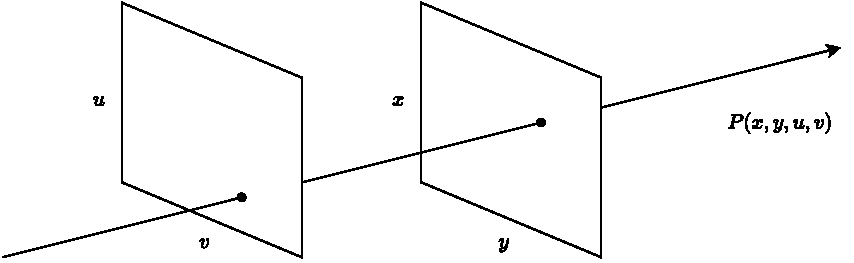
\includegraphics[width=0.95\linewidth]{figures/chapter2/double_plane_model.drawio}
	\bicaption
	{光场双平面四参数模型\upcite{levoy2023light}}
	{Light field biplane four-parameter model\upcite{levoy2023light}}  
	\label{chapter2_fig1:double_plane}
\end{figure}


五维光场模型通过记录红、绿、蓝三原色来简化波长$\lambda$,以及通过记录不同帧来简化时间$t$。
实际上,光线在空间传播中,因传播距离而造成的信息损耗微乎其微,光场模型还可以进一步简化。
Levoy等\upcite{levoy2023light}忽略掉传播距离维度$z$得到四维光场模型,
同时提出光场渲染理论和双平面模型来描述静态的可见光,
如图~\ref{chapter2_fig1:double_plane}~所示。
双平面模型利用两个互相平行的参数化平面表示四维光场。
假设光线在没有遮挡物和散射介质的区域,忽略光线在传播过程中波长和时间维度的变化,
则任意一个包含位置和方向信息的光线都可以用双平面参数来表示,
空间中的光线穿过这两个平面分别相交于点$(u, v)$和点$(s, t)$,
光线即可用四维光场函数表示,其模型参数如下:
\begin{equation}
	P(u, v, x, y)
\end{equation}




%%%%%%%%%%%%%%%%%%%%%%%%%%%%%%%%%%%%%%%%%%%%%%%%%%%
%%
%% Split paragraphs
%%
%%%%%%%%%%%%%%%%%%%%%%%%%%%%%%%%%%%%%%%%%%%%%%%%%%%


在光场成像设备中,可以用$(u, v)$表示光线与微透镜阵列的交点,用$(s, t)$表示光线与CCD传感器探测面的交点。
一条光线在整个四维空间中对应着光场的一个采样点。四维光场理论的推出为全光相机、相机阵列等设备提供了理论基础。目前,大多数单体全光相机和相机阵列的光场采集设备都遵循着四维光场理论。
%
%
%发展出了适用于光学系统的光场双平面参数特征。
%假设一条光线在两个不共面的平面$(u,v)$和平面$(s,t)$各有一个交点,则该光线可以用这两个交点唯一表示。
%光场是计算机科学领域的学者定义的“Light Field”,是指除了包含原图像矩阵中的空间坐标$(x,y)$和强度$I$外,还有光线入射的角度信息$(\theta,\varphi)$。
%光在传播过程中的各种潜在的视觉属性(如运动、颜色和方向)。




%%%%%%%%%%%%%%%%%%%%%%%%%%%%%%%%%%%%%%%%%%%%%%%%%%%
%%
%% Split paragraphs
%%
%%%%%%%%%%%%%%%%%%%%%%%%%%%%%%%%%%%%%%%%%%%%%%%%%%%


%%%%%%%%%%%%%%%%%%%%%%%%%%%%%%%%%%%%%%%%%%%%%%%%%%%%%%%%%%%%%%%%%%%%%%%%%%%%
\BiSubsection{光场成像原理}
{Principles of Light Field Imaging}

在传统成像中,光线被捕获并呈现到成像平面上。然而,光场成像采用不同的方式。
它是一种计算成像技术,旨在捕获光线强度的同时记录光线的传播方向。
为了得到可视化的图像信息,必须对捕获的光场信息进行计算处理。
根据成像设备或记录方法的不同,现有的光场成像方式可以分为多传感器采集成像、
时间序列采集成像、空域复用成像和频域复用成像。





%%%%%%%%%%%%%%%%%%%%%%%%%%%%%%%%%%%%%%%%%%%%%%%%%%%
%%
%% Split paragraphs
%%
%%%%%%%%%%%%%%%%%%%%%%%%%%%%%%%%%%%%%%%%%%%%%%%%%%%




\begin{figure}[b]
	\centering
	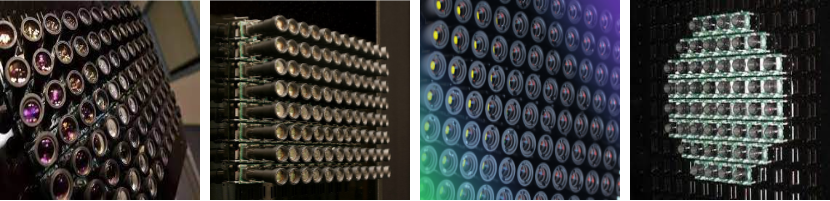
\includegraphics[width=1\linewidth]{figures/chapter2/camera_array}
	\bicaption{相机阵列光场成像}{Camera array for light field imaging}  
	\label{chapter2_fig2:camera_array}
\end{figure}




%%%%%%%%%%%%%%%%%%%%%%%%%%%%%%%%%%%%%%%%%%%%%%%%%%%
%%
%% Split paragraphs
%%
%%%%%%%%%%%%%%%%%%%%%%%%%%%%%%%%%%%%%%%%%%%%%%%%%%%


%%%%%%%%%%%%%%%%%%%%%%%%%%%%%%%%%%%%%%%%%%%%%%%%%%%%%%%%%%%%%%%%%%%%%%%%%
(1)
相机阵列光场成像


%
%使用相机阵列获取光场信息是通过多个相机以特定的空间分布在不同视角下捕获场景图像的方法,
%
%每个相机捕获的是四维光场在其相对于场景方向上的二维投影。
%通过融合这些相机捕获的图像,就可以获得完整的四维光场数据。
%大尺度空间相机阵列主要应用于合成孔径成像以实现“透视”监测,或通过拼接实现大视角全景成像。
%相比之下,紧密排列的相机阵列则主要用于捕获高性能动态场景或场景的三维分布和结构等信息。
%光场数据的空间解析度取决于传感器本身,而角度解析度由传感器数量和布局方式确定。
%这种采集方法能够在单次曝光中瞬时捕捉光场,因此还能记录光场的时间序列信息。
%尽管这种成像方法空间解析度较高,但却带来了庞大的图像数据量,因此处理上更加耗时。
%此外,这种成像方式对多传感器的相对位置要求也较高。 
%


使用相机阵列获取光场信息是一种最为简易的方式,
通过排列多个普通平面相机组成相机阵列,如图~\ref{chapter2_fig2:camera_array}~所示。
每一个平面相机捕获的图像,隶属于四维光场中在固定角度位置的成像。
组合所有的图像构成图像阵列,就构成了完整的光场数据。
这种方式,需要每个平面相机具有相同的成像分辨率,
其视角差异跟相机阵列的排列相关,排列的紧密与否决定了形成光场数据的角度维度的精细程度。
同时,这种成像方式,需要校准每个相机的空间位置,实际实现上往往具有较大的空间误差,
因为每个相机需要在三维空间位置对齐,其接收入射光线的角度也需要固定,
实际使用时,容易在成像阶段引入噪声。
排列的阵列相机,存在木桶效应,即如果有一个相机无法正常工作,
其位置所在的行和列的其他相机所获取的光场信息都会受不同程度的损失。







%%%%%%%%%%%%%%%%%%%%%%%%%%%%%%%%%%%%%%%%%%%%%%%%%%%
%%
%% Split paragraphs
%%
%%%%%%%%%%%%%%%%%%%%%%%%%%%%%%%%%%%%%%%%%%%%%%%%%%%





\begin{figure}[t]
	\centering
	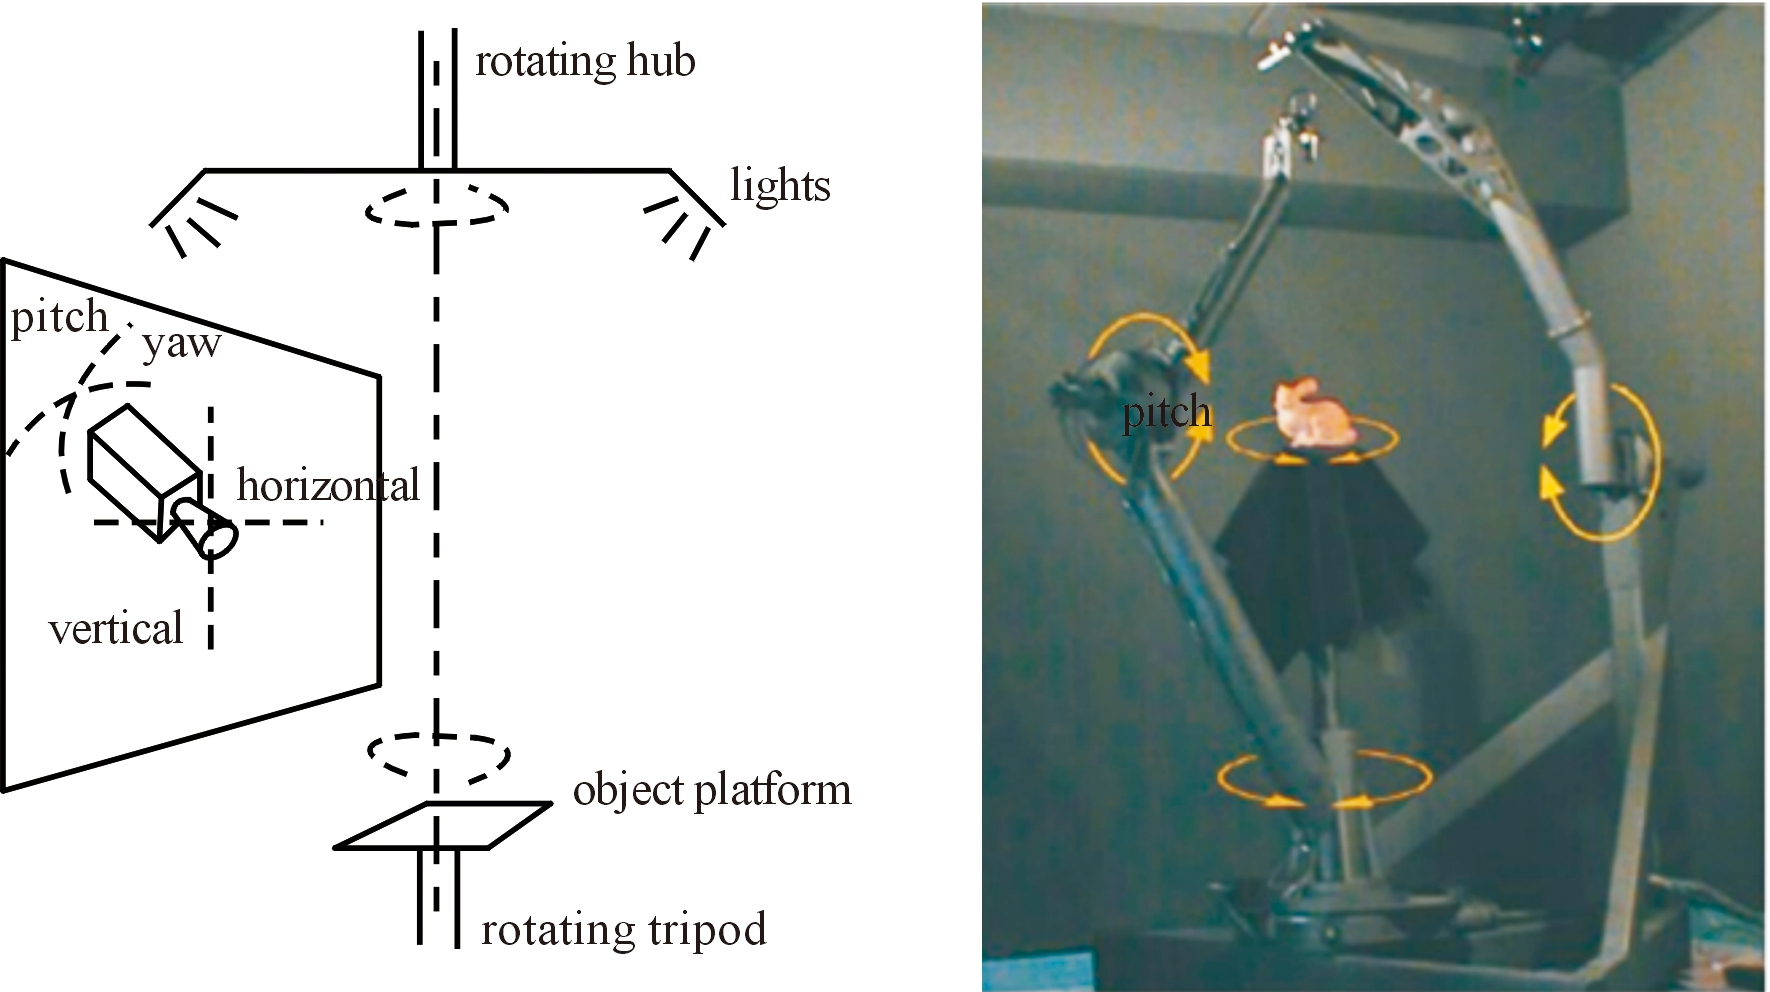
\includegraphics[width=0.75\linewidth]{figures/chapter2/time_seq2}
	\bicaption{时间序列光场成像\upcite{levoy2023light}}
	{Time-series light field imaging\upcite{levoy2023light}}  
	\label{chapter2_fig3:time_seq2}
\end{figure}



%%%%%%%%%%%%%%%%%%%%%%%%%%%%%%%%%%%%%%%%%%%%%%%%%%%%%%%%%%%%%%%%%%%%%%%%%%%%%%%%%
(2)
时间序列成像


除了多个相机阵列排布外,Marc Levoy等人\upcite{levoy2023light}采用了单相机扫描系统。
他们通过让相机在固定的导轨上移动,
能够在不同的空间视角下拍摄图片,并添加时间信息,
最后将这些图像进行融合,从而实现相同的功能。
图~\ref{chapter2_fig3:time_seq2}~是典型的时序采集光场信息的示例。
与使用相机阵列的多传感器采集方式相比,
时间序列成像不局限于固定的空间位置,
能够实现低视差、高角度范围的图像采集,
但是,这种方法也有弊端,
即相机移动的控制结构需要高精度的控制,
同时,这些附加的空间坐标信息,角度信息也需要附加到图像数据中,
使得这种成像方式比较耗时。
这些确定使得这种图像采集方式更适合静态场景的光场信息获取。






%%%%%%%%%%%%%%%%%%%%%%%%%%%%%%%%%%%%%%%%%%%%%%%%%%%
%%
%% Split paragraphs
%%
%%%%%%%%%%%%%%%%%%%%%%%%%%%%%%%%%%%%%%%%%%%%%%%%%%%






%%%%%%%%%%%%%%%%%%%%%%%%%%%%%%%%%%%%%%%%%%%%%%%%%%%%%%%%%%%%%%%%%%%%%%%%%%%%%%%%%%%%%%%%%%%
(3)
微透镜光场成像


微透镜成像方式也叫空域复用成像方式,这是光场采集中常见的方式之一。
图~\ref{chapter2_fig4:microlens_for_lf_imaging}~展示了微透镜光场成像方式的工作原理。
普通的成像系统能够通过入射光线而成像,
微透镜光场成像扩展了普通成像系统,
为了获取不同视角的成像,
将微透镜阵列添加在普通成像系统的主透镜后,
每个微透镜都有相应的CMOD传感器记录光线信息,
就能获取不同空间位置和光线方向的四维光场数据。
微透镜成像方式具有空间体积小,成像设备便携易使用等特点,
一次拍摄就可以直接获取光场成像所需的全部数据。
这种成像方式最早在1992年由Adelson\upcite{adelson1992single}及其团队提出。
这种成像方式的缺点是视角差异有限,具体跟微透镜的数量相关,
且微透镜之间的距离固定。
后来出现了微透镜和传感器直接距离可调的光场相机结构,
使得能够设置主透镜的聚焦范围,实现了更为灵活的光场信息采集方式。




\begin{figure}[t]
	\centering
	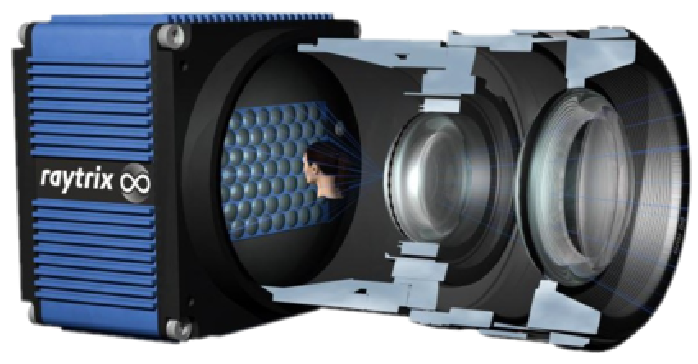
\includegraphics[width=0.65\linewidth]{figures/chapter2/microlens_for_lf_imaging2.drawio}
	\bicaption{微透镜光场成像\upcite{adelson1992single}}
	{Microlens light field imaging\upcite{adelson1992single}}  
	\label{chapter2_fig4:microlens_for_lf_imaging}
\end{figure}






%
% 相机阵列的体积庞大,限制了其应用范围。
% 通过缩小相机阵列中各成像单元之间的基线,可以在单个相机框架下利用微透镜阵列来采集光场信息。
% 空域复用的成像方式通过在图像传感器上安装微透镜阵列来实现,这是光场采集中常见的方式之一,可通过单次曝光捕获光场信息。
%
%


%%%%%%%%%%%%%%%%%%%%%%%%%%%%%%%%%%%%%%%%%%%%%%%%%%%
%%
%% Split paragraphs
%%
%%%%%%%%%%%%%%%%%%%%%%%%%%%%%%%%%%%%%%%%%%%%%%%%%%%



%%%%%%%%%%%%%%%%%%%%%%%%%%%%%%%%%%%%%%%%%%%%%%%%%%%%%%%%%%%%%%%%%%%%%%%%%%%%
\BiSubsection{光场数据的可视化}{Visualization of Light Field Data}

根据先前的描述,四维模型中双平面光场模型是目前广泛采用的光场模型,其中两个维度表示空间位置,另外两个维度表示方向角度。
在三维世界中,描绘四维光场数据是具有挑战性的,可以通过固定双平面光场模型的任意两个维度来展示二维切片以可视化光场数据。
虽然二维光场切片无法传达完整的光场信息,但可以帮助解释光场数据的内在特征。
固定角度维度可以获得子孔径图像阵列形式的光场数据;固定空间维度可以获得宏像素形式的光场数据;固定一个角度维度和一个空间维度可以获得包含空间和角度信息的 EPI 形式的光场数据。焦点堆栈数据也是一种光场可视化的形式。
常用的光场可视化方式主要有子孔径图像阵列形式、宏像素形式、极线图形式和焦点堆栈。



%%%%%%%%%%%%%%%%%%%%%%%%%%%%%%%%%%%%%%%%%%%%%%%%%%%
%%
%% Split paragraphs
%%
%%%%%%%%%%%%%%%%%%%%%%%%%%%%%%%%%%%%%%%%%%%%%%%%%%%





(1)
子孔径图像


%%%%%%%%%%%%%%%%%%%%%%%%%%%%%%%%%%%%%%%%%%%%%%%%%%%
%%
%% Split paragraphs
%%
%%%%%%%%%%%%%%%%%%%%%%%%%%%%%%%%%%%%%%%%%%%%%%%%%%%





子孔径图像阵列视图是广泛使用的光场可视化方法之一。
固定角度维度$(u, v)$,令$u = u^{*}$,$ v = v^{*} $,
则$P(u^{*}, v^{*}, x, y) $表示在单个视点$(u^{*}, v^{*})$下的图像$(x,y)$。
若把$(x,y)$看成传统相机所成的像,$(u, v)$就表示相机所在的位置。
光场$P(u, v, x, y)$就可以理解为相机在视点平面等间隔采样,表现为相机不同视点$(u, v)$位置处所捕获的图像。
光场相机进行子孔径成像,
可以记录不同空间角度的彩色图像,
学名子孔径图像,
又被称为亚光圈图像,简称为视图。
如图~\ref{chapter2_fig5:multi_photo}~所展示。
图中右侧显示了以中心视点(5, 5)为基准的亚光圈图像的可视化图。




%%%%%%%%%%%%%%%%%%%%%%%%%%%%%%%%%%%%%%%%%%%%%%%%%%%
%%
%% Split paragraphs
%%
%%%%%%%%%%%%%%%%%%%%%%%%%%%%%%%%%%%%%%%%%%%%%%%%%%%






\begin{figure}[!ht]
	\centering
	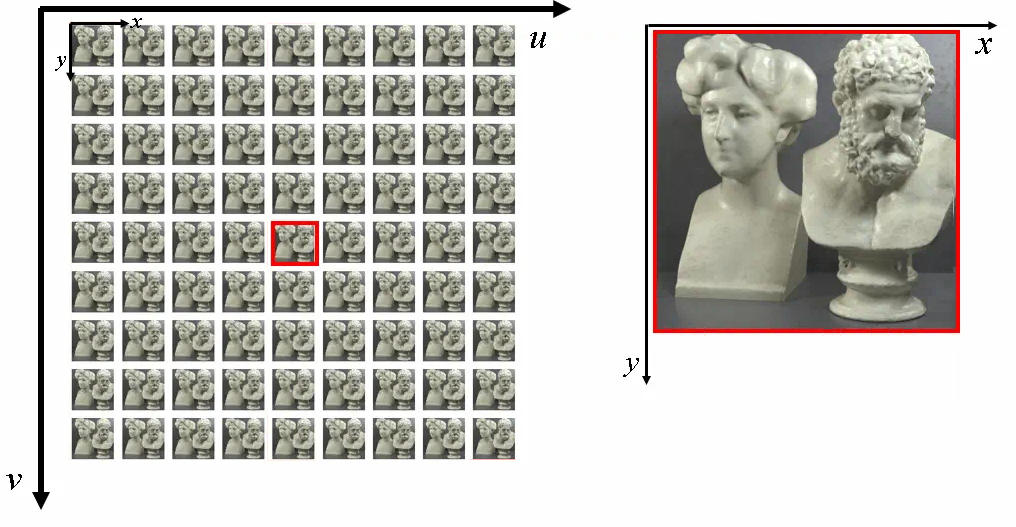
\includegraphics[width=0.75\linewidth]{figures/chapter2/multi_photo}
	\bicaption{子孔径图像阵列形式的光场数据可视化}
	{Visualization of light field data in the form of subaperture image arrays}  
	\label{chapter2_fig5:multi_photo}
\end{figure}
%
%
%
%
\begin{figure}[!ht]
	\centering
	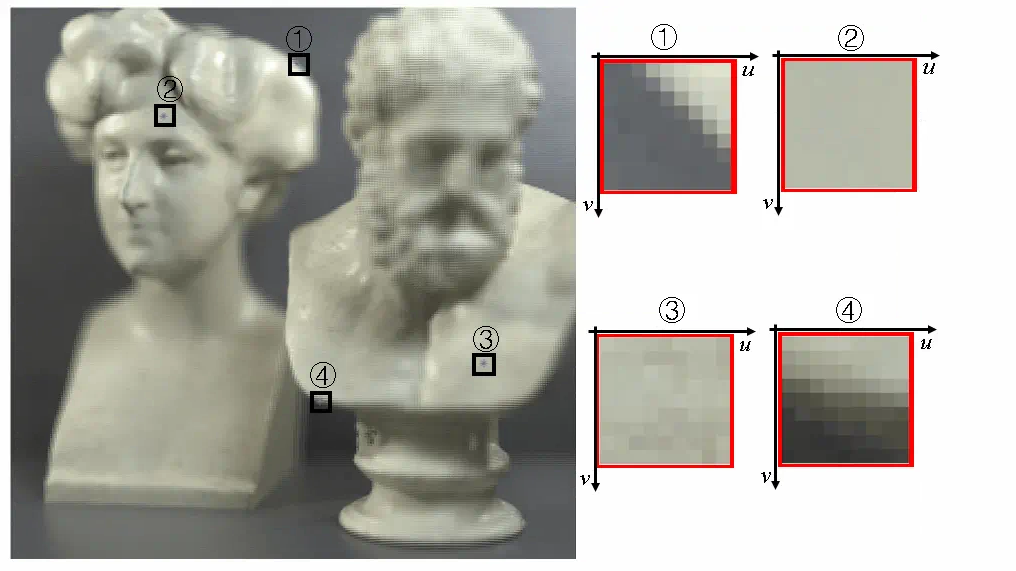
\includegraphics[width=0.80\linewidth]{figures/chapter2/macro_photo}
	\bicaption{宏像素形式的光场数据可视化}
	{Visualizing light field data in macropixel form}  
	\label{cpt2_fig5:macro_photo}
\end{figure}
%
%
%multi_photo
%
%

%%%%%%%%%%%%%%%%%%%%%%%%%%%%%%%%%%%%%%%%%%%%%%%%%%%
%%
%% Split paragraphs
%%
%%%%%%%%%%%%%%%%%%%%%%%%%%%%%%%%%%%%%%%%%%%%%%%%%%%


(2)
宏像素视图


%%%%%%%%%%%%%%%%%%%%%%%%%%%%%%%%%%%%%%%%%%%%%%%%%%%
%%
%% Split paragraphs
%%
%%%%%%%%%%%%%%%%%%%%%%%%%%%%%%%%%%%%%%%%%%%%%%%%%%%



宏像素视图是另一种光场可视化形式。固定空间维度的坐标$(x, y)$,令$x=x^{*}$,$y=y^{*}$,
则$ P(u, v, x^{*}, y^{*})$可以表示为单个宏像素,
通过按照空间分辨率遍历所有宏像素,并按照图像顺序排列,形成宏图像。
如图~\ref{cpt2_fig5:macro_photo}~所示。
每个宏像素在宏图像中的分辨率代表了光场的角度分辨率。
%
不考虑遮挡的情况,$ P(u, v, x^{*}, y^{*})$表示场景中某一物点在所有视点下对应的像素值,
即$ P(u, v, x^{*}, y^{*})$表示光场采集设备所捕获到的物点发出的所有光线,
如图~\ref{cpt2_fig5:macro_photo}~中标号\ding{193}、\ding{194}的宏像素所示。
考虑遮挡的情况,$ P(u, v, x^{*}, y^{*})$可由场景中的某一遮挡物点,
在可视点下对应的像点和在非可视点下其他物点对应的像点的组合,
在图~\ref{cpt2_fig5:macro_photo}~中标号\ding{192}、\ding{195}的宏像素中,
可以看到宏像素内含有不同物点发出的光线。\par
%
%
%
%
%
\begin{figure}[!ht]
	\centering
	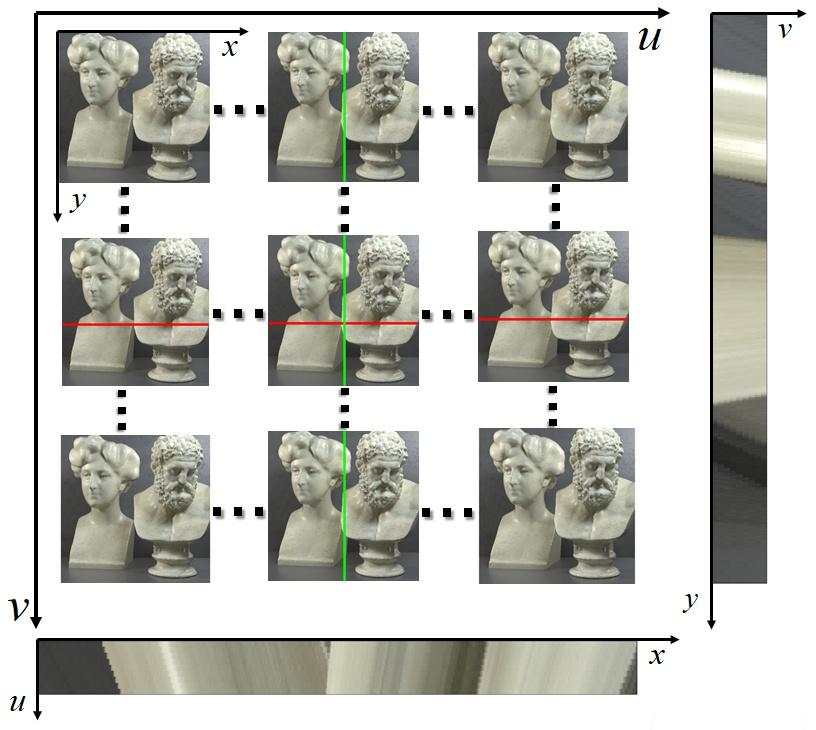
\includegraphics[width=0.75\linewidth]{figures/chapter2/epi_photos}
	\bicaption{极视角形式的光场数据可视化}
	{Light field data visualization in polar perspective form}  
	\label{cpt2_fig6:epi_photos}
\end{figure}
%
%
%




%%%%%%%%%%%%%%%%%%%%%%%%%%%%%%%%%%%%%%%%%%%%%%%%%%%
%%
%% Split paragraphs
%%
%%%%%%%%%%%%%%%%%%%%%%%%%%%%%%%%%%%%%%%%%%%%%%%%%%%



(3)极平面图


%%%%%%%%%%%%%%%%%%%%%%%%%%%%%%%%%%%%%%%%%%%%%%%%%%%
%%
%% Split paragraphs
%%
%%%%%%%%%%%%%%%%%%%%%%%%%%%%%%%%%%%%%%%%%%%%%%%%%%%



极平面视图(Epipolar-Plane Images, EPI)。
在四维光场表示下,
分别固定一个角度维度和一个空间维度,
即可获取极平面视图表示。
具体来说,
当固定$(v, y)$坐标,令$v=v^{*}$,$y=y^{*}$,
则$ P(u, v^{*}, x, y^{*})$被称为固定$(v^{*}, y^{*})$的极平面图像,即垂直方向上的EPI图像。
同理,当固定$(u, x)$,则$ P(u^{*}, v, x^{*}, y)$被称为固定$(u^{*}, x^{*})$的极平面图像,
即水平方向上的EPI图像。
如图~\ref{cpt2_fig6:epi_photos}~所示,
基于四维度光场数据表示,
通过逐行索引像素或者逐列堆叠像素,即可形成极平面图,
如图中右侧和下侧所示。
这样堆叠出的像素平面图能够反应像素点在现实场景中的相对位置信息。








%%%%%%%%%%%%%%%%%%%%%%%%%%%%%%%%%%%%%%%%%%%%%%%%%%%
%%
%% Split paragraphs
%%
%%%%%%%%%%%%%%%%%%%%%%%%%%%%%%%%%%%%%%%%%%%%%%%%%%%





\begin{figure}[b]
	\centering
	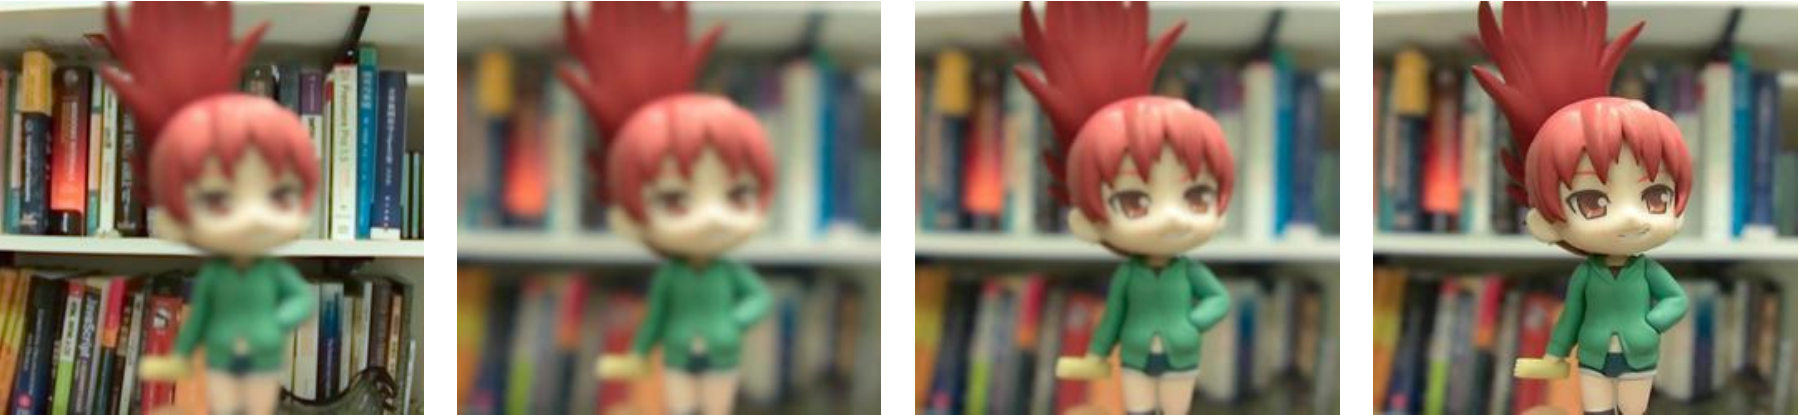
\includegraphics[width=0.95\linewidth]{figures/chapter2/focal_stack}
	\bicaption{焦点堆栈形式的光场数据可视化}
	{Visualization of light field data as focus stack}  
	\label{cpt2_fig7:focal_stack}
\end{figure}



%%%%%%%%%%%%%%%%%%%%%%%%%%%%%%%%%%%%%%%%%%%%%%%%%%%
%%
%% Split paragraphs
%%
%%%%%%%%%%%%%%%%%%%%%%%%%%%%%%%%%%%%%%%%%%%%%%%%%%%



(4)
焦点堆栈



%%%%%%%%%%%%%%%%%%%%%%%%%%%%%%%%%%%%%%%%%%%%%%%%%%%
%%
%% Split paragraphs
%%
%%%%%%%%%%%%%%%%%%%%%%%%%%%%%%%%%%%%%%%%%%%%%%%%%%%



焦点堆栈是由不同散焦图片组成。
是目前常用的光场数据的中间表示格式。
不同的散焦图片具有局部聚焦的效果,如图~\ref{cpt2_fig7:focal_stack}~所示,
根据景深的不同,即不同散焦图片实际所属的聚焦平面的远近不同,
来依次排列出焦点堆栈。
在这些图像中,聚焦于物体深度的部分呈现清晰度,而非聚焦部分则显得模糊。
由于“近大远小”效应,不同图像之间存在放大比例差异。
放大比例记录了光线传播方向的信息,这些存在的放大比例可以进行光场的重投影。
但是一般并不仅仅使用焦点堆栈来表示完备的光场数据,
还会辅以全聚焦图,
即一张彩色图片,其场景中所示物体都是以清晰的状态呈现。
全聚焦图和焦点堆栈相辅相成,一个对于整体场景的清晰表示,
一个对应场景中不同景深下的局部表示。



%%%%%%%%%%%%%%%%%%%%%%%%%%%%%%%%%%%%%%%%%%%%%%%%%%%
%%
%% Split paragraphs
%%
%%%%%%%%%%%%%%%%%%%%%%%%%%%%%%%%%%%%%%%%%%%%%%%%%%%



%
%
%
%\textcolor{red}{TODO}
%
%搜集聚焦堆栈数据的方法包括移动镜头或探测器,以采集在不同成像平面上聚焦的图像序列。在这些图像中,聚焦于物体深度的部分呈现清晰度,而非聚焦部分则显得模糊。由于“近大远小”效应,不同图像之间存在放大比例差异。放大比例记录了光线传播方向的信息,只有在存在放大比例时才能进行光场的重投影;而利用光场重聚焦技术(例如,位移和叠加)生成的重聚焦数据则不包含放大比例信息,能够用于深度重建,但无法重新投影出完整的光场。然而,对于深度重建来说,放大比例本身并无实际帮助。
%
%
%
%当固定x=x0, u=u0时,按照空间和方向的顺序排列在一起,就可以得到垂直方向的EPI图像;当固定y=y0, v=v0时,通过改变x的u的顺序,就能得到水平方向的EPI图像。当物体满足朗伯体表现的性质,即向各个方向发出的光线强度相等时,那么该点在极平面图像中被表示为一条直线,该直线的斜率可以反映出该点的深度信息。图2.6展示了一个极平面图像的例子。
%
%
%通过逐个选择所有单视角图像,便可以构建多角度视图。单个视角图像类似于RGB图像,可以呈现所拍摄场景的空间信息。这种固定方向参数、遍历所有可选单视角图像的方法称为多视角图像的多视图表示。当设定代表光场空间的两个维度为x = x0,y = y0时,可以得到单个宏像素。通过按照空间分辨率遍历所有宏像素,并按照图像顺序排列,形成宏图像。
%每个宏像素在宏图像中的分辨率代表了光场的角度分辨率,属于多角度视图的角度域表示法。图中展示的3x3角度分辨率和空间分辨率的多角度视图示例,其中(a)表示多视图表示法,(b)代表角度域表示法。
%
%
%
%
%
%当设定代表光场方向的两个维度参数为u = u0,v = v0时,就可以获得单个视角图像。
%
%
%
%






%%%%%%%%%%%%%%%%%%%%%%%%%%%%%%%%%%%%%%%%%%%%%%%%%%%
%%
%% Split paragraphs
%%
%%%%%%%%%%%%%%%%%%%%%%%%%%%%%%%%%%%%%%%%%%%%%%%%%%%




%%%%%%%%%%%%%%%%%%%%%%%%%%%%%%%%%%%%%%%%%%%%%%%%%%%%%%%%%%%%%%%%%%%%%%%%%%%%
\BiSection{光场显著性目标检测算法原理}
{Principle of Light Field Salient Object Detection Algorithm}

%
%{光场显著性目标检测相关理论}
%{Related Theories on Light Field Salient Object Detection}
%
%
%
%
%
前文已指出,光场数据常用的
子孔径图像、
宏像素视图、
极平面图和
焦点堆栈
四种表示方式,其中宏像素视图成像出的多视角图像和焦点堆栈数据常用于显著性目标检测。
本小节探讨了基于这两种光场数据形式的显著性目标检测算法原理。



%,并介绍了评估光场显著性目标检测的指标。
%
%
%前文已指出,光场数据常用三种方式表示,其中多视角图像和焦点堆栈数据常用于显著性目标检测。
%本节首先探讨了基于这两种光场数据形式的显著性目标检测原理,并最后介绍了评估光场显著性目标检测的指标。
%常用的光场可视化方式主要有子孔径图像阵列形式、宏像素形式、极线图形式和焦点堆栈。






%%%%%%%%%%%%%%%%%%%%%%%%%%%%%%%%%%%%%%%%%%%%%%%%%%%
%%
%% Split paragraphs
%%
%%%%%%%%%%%%%%%%%%%%%%%%%%%%%%%%%%%%%%%%%%%%%%%%%%%




%%%%%%%%%%%%%%%%%%%%%%%%%%%%%%%%%%%%%%%%%%%%%%%%%%%%%%%%%%%%%%%%%%%%%%%%%%%%%%%%%%
\BiSubsection{基于多视角图像的显著性目标检测原理}
{Principles of Salient Object Detection via Multi-view Images}


基于多视角图像的显著性目标检测方法主要利用视差与深度之间的关系,在网络模型中引入了场景结构的线索。
通常,通过编码网络来提取多视角图像的高阶和低阶特征,并结合深度线索挖掘出的角度特征来定位显著性目标。
多视角图像的深度线索是通过不同视角之间的视差引入的。

\begin{figure}[b]
	\centering
	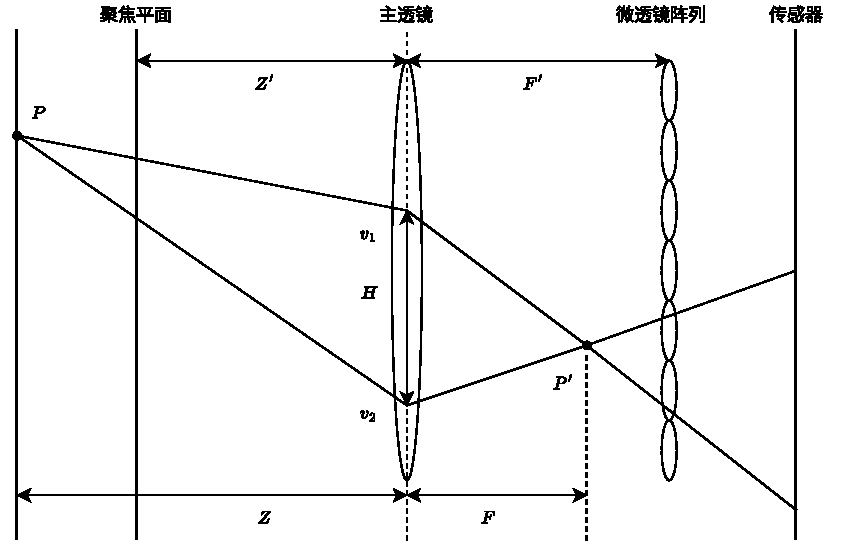
\includegraphics[width=0.90\linewidth]{figures/chapter2/microlens_array_imaging.drawio}
	\bicaption{基于微透镜阵列的光场相机成像原理\upcite{adelson1992single}}
	{Imaging principle of light field camera based on microlens array\upcite{adelson1992single}}  
	\label{cpt2_fig8:multi_array}
\end{figure}

具体来说,如图~\ref{cpt2_fig8:multi_array}~所示,
在观察同一目标$P$时,考虑两个视角 $v_{1}$ 和 $v_{2}$,
目标经过主透镜成像后形成像素点$P'$,
其中目标$P$到主透镜的距离为$Z$,而$Z'$表示主透镜到聚焦平面的距离,
主透镜到成像点的距离为$F$,主透镜到微透镜阵列的距离为$F'$。
两视点之间的距离用$H$表示,由此可推导出如下几何关系:
%
%
\begin{equation}
	\frac{D}{H} = \frac{F'}{Z'} - \frac{F'}{Z} 
	\label{cpt2_fac1:relate}
\end{equation}
%
%
其中$D$表示视差,$F'$、$H$和$Z'$都是相机内参,用来计算目标$P$点的深度。



%%%%%%%%%%%%%%%%%%%%%%%%%%%%%%%%%%%%%%%%%%%%%%%%%%%
%%
%% Split paragraphs
%%
%%%%%%%%%%%%%%%%%%%%%%%%%%%%%%%%%%%%%%%%%%%%%%%%%%%





从公式~\ref{cpt2_fac1:relate}~可以看出,
相机的成像参数对于如何成像发挥着重要作用。
张等研究者\upcite{zhang2022exploring}所提出的 ESCNet网络,
通过组合网络来实现光场显著性目标检测。
先使用网络进行光场原生数据的高维特征提取,生成可靠的4D光场信息;
再构造网络合成每一个多视角切片的显著语义信息
充分利用多个视点之间的空间相关性,构造基于信息整合光场显著性目标检测网络。






%%%%%%%%%%%%%%%%%%%%%%%%%%%%%%%%%%%%%%%%%%%%%%%%%%%
%%
%% Split paragraphs
%%
%%%%%%%%%%%%%%%%%%%%%%%%%%%%%%%%%%%%%%%%%%%%%%%%%%%



%%%%%%%%%%%%%%%%%%%%%%%%%%%%%%%%%%%%%%%%%%%%%%%%%%%%%%%%%%%%%%%%%%%%%%%%%%%%
\BiSubsection{基于焦点堆栈的显著性目标检测原理}
{Principles of Salient Object Detection via Focus Stack}

  
当前,大多数光场显著性目标检测算法使用混合模态来构建网络,
网络可以同时输入全聚焦图片和焦点堆栈.
这种方法主要依赖于多焦特性,即场景聚焦于焦点堆栈中不同深度的目标,
通过探索其中蕴藏的场景结构信息,
来增强网络对于图片中场景的理解,以生成高质量的显著性预测图。



%%%%%%%%%%%%%%%%%%%%%%%%%%%%%%%%%%%%%%%%%%%%%%%%%%%
%%
%% Split paragraphs
%%
%%%%%%%%%%%%%%%%%%%%%%%%%%%%%%%%%%%%%%%%%%%%%%%%%%%


早期的光场显著性目标检测还未引入深度卷积神经网络,
提取光场数据的特征使用硬性的手动处理,
依赖不同的色彩、对比度、区域等先验信息来编码全聚焦图像,
然后逐帧处理焦点堆栈序列,通过点扩散函数表示每张散焦图片的聚焦程度,
来综合判断场景中的显著性物体。
本文通过PANet\upcite{piao2021panet}模型来阐述这一方式的原理。
在PANet中,网络通过相比图片帧更细化的方式,即区域级的聚焦度量方式,
其通过全聚焦支路的特征信息与每个焦点堆栈图片语义特征的比较,
来判断不同散焦图片中显著清晰区域的位置,
最后将这些不同区域的特征权重加以整合,
进行两个支路的信息融合,如图~\ref{cpt2_fig9:model_of_fs_inputs}~中所示,
就能实现网络对于聚焦区域的场景感知。


%%%%%%%%%%%%%%%%%%%%%%%%%%%%%%%%%%%%%%%%%%%%%%%%%%%
%%
%% Split paragraphs
%%
%%%%%%%%%%%%%%%%%%%%%%%%%%%%%%%%%%%%%%%%%%%%%%%%%%%




基于Transformer架构的光场显著性目标检测网络,
通常依赖Transformer架构的长距离建模能力,
在网络的解码器添加Transformer块来聚合全部焦点堆栈的信息。
以LFTransNet网络\cite{liu2023lftransnet}为例,
网络通过可学习的权重作为查询,输入到Transformer块中,查询
全部焦点堆栈特征来学习一个差异化通道权重,
经过若干层特征提取后,将这个差异化权重加权到焦点堆栈特征上,
来增强焦点堆栈特征的显著性表示,
最后再融合两个支路的预测信息,
并通过显著性预测头产生最终的显著性预测。



%%%%%%%%%%%%%%%%%%%%%%%%%%%%%%%%%%%%%%%%%%%%%%%%%%%
%%
%% Split paragraphs
%%
%%%%%%%%%%%%%%%%%%%%%%%%%%%%%%%%%%%%%%%%%%%%%%%%%%%





\begin{figure}[t]
	\centering
	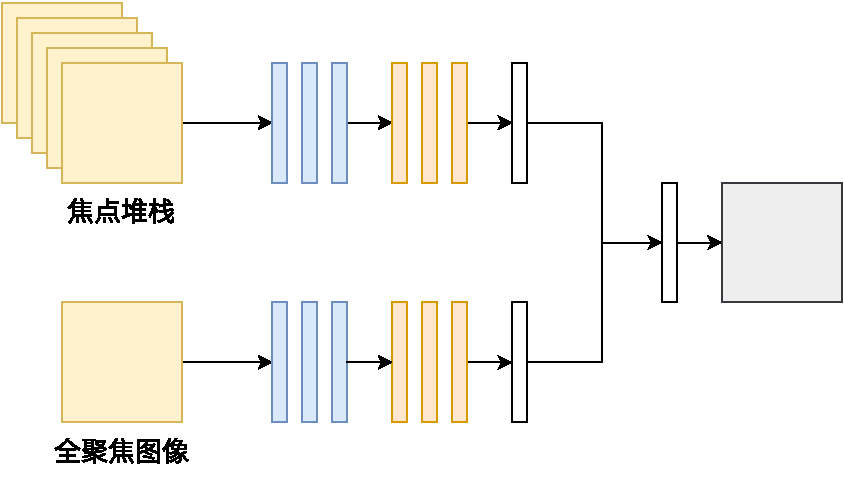
\includegraphics[width=0.70\linewidth]{figures/chapter2/model_of_fs_inputs}
	\bicaption{基于焦点堆栈的光场显著性目标检测模型\upcite{piao2021panet}}
	{Light field salient object detection model based on focus stack\upcite{piao2021panet}}  
	\label{cpt2_fig9:model_of_fs_inputs}
\end{figure}



%%%%%%%%%%%%%%%%%%%%%%%%%%%%%%%%%%%%%%%%%%%%%%%%%%%
%%
%% Split paragraphs
%%
%%%%%%%%%%%%%%%%%%%%%%%%%%%%%%%%%%%%%%%%%%%%%%%%%%%




%%%%%%%%%%%%%%%%%%%%%%%%%%%%%%%%%%%%%%%%%%%%%%%%%%%%%%%%%%%%%%%%%%%%%%%%%%%%
\BiSection{显著性目标检测性能评估指标}
{Performance Evaluation Metrics for Salient Object Detection}



为了全面评估各种显著性目标检测模型在不同数据集上的分割性能,
本节将介绍显著性目标检测任务中广泛使用的五种评估指标。
分别包括
平均绝对误差(Mean Absolute Error,MAE)、
精确率-召回率曲线(P-R曲线)、
F-measure\upcite{achanta2009frequency}、
加权的F-measure\upcite{margolin2014evaluate}、
E-measure\upcite{fan2018enhanced}和
S-measure\upcite{fan2017structure}。



%%%%%%%%%%%%%%%%%%%%%%%%%%%%%%%%%%%%%%%%%%%%%%%%%%%
%%
%% Split paragraphs
%%
%%%%%%%%%%%%%%%%%%%%%%%%%%%%%%%%%%%%%%%%%%%%%%%%%%%





%%%%%%%%%%%%%%%%%%%%%%%%%%%%%%%%%%%%%%%%%%%%%%%%%%%%%%%%%%%%%%%%%%%%%%%%%%%%%%%
(1)平均绝对误差\par
平均绝对误差通过衡量显著性预测图与相应的真实值之间的平均每个像素点绝对差异来
直观的评估显著性图的质量。
它是评估预测质量的最简单有效的方式。
该评估指标的公式如下:
\begin{equation}
	MAE=\frac{1}{W \times H}\sum_{i=1}^{W} \sum_{j=1}^{H} \left |  \hat{S} (i,j) - S(i,j)\right | 
\end{equation}
%
%
其中$\hat{S}(i,j)$和$S(i,j)$分别表示显著性预测图和相应真值图对应坐标的像素。
值得一提的是,当该性能指标的值越低时,意味着预测图越接近真值图。
平均绝对误差展现了出色的可解释性,因为它直接展示了模型预测值与实际值之间的差异大小,
有助于让研究者更加直观地评估模型的性能。
需要留意的是,平均绝对误差对异常值比较敏感,因为它会均等对待每个样本的误差。
若数据集包含异常值,这将会对平均绝对误差的计算结果造成较大影响。



%%%%%%%%%%%%%%%%%%%%%%%%%%%%%%%%%%%%%%%%%%%%%%%%%%%
%%
%% Split paragraphs
%%
%%%%%%%%%%%%%%%%%%%%%%%%%%%%%%%%%%%%%%%%%%%%%%%%%%%




%%%%%%%%%%%%%%%%%%%%%%%%%%%%%%%%%%%%%%%%%%%%%%%%%%%%%%%%%%%%%%%%%%%%%%%%%%%%%%%
(2)精确率-召回率曲线(P-R曲线)\par
%
%
P-R 曲线是用来评估预测图的精准率和召回率的工具。
%P-R曲线就是精确率和召回率的曲线,
曲线以召回率作为横坐标轴,以精确率作为纵坐标轴。
在评估二分类任务时,通常会构造混淆矩阵加以分析,
精确率和召回率可以从混淆矩阵中计算而来,公式如下:
%
%
\begin{equation}
	Precision = \frac{TP}{TP + FP},~Recall = \frac{TP}{TP+FN}
\end{equation}
%
%
其中分类器把正例正确地分类为正例TP(True Positive),
把正例错误地分类为负例,标记为FN(False Negative),
把负例正确地分类为负例,用TN(True Negative)表示,
FP(False Positive)表示
把负例错误分类为正例。
算法对样本进行分类时,都会有置信度,即表示该样本是正样本的概率,
比如0.99的概率认为样本A是正例,0.01的概率认为样本B是正例。
通过选择合适的阈值,比如以0.5为阈值对样本进行划分,
预测置信度大于0.5的就认为是正例,小于0.5的就是负例。
通过置信度就可以对所有样本进行排序,再逐个样本的选择阈值,
在该样本之前的都属于正例,该样本之后的都属于负例。
每一个样本作为划分阈值时,都可以计算对应的Precision和Recall,
那么就可以以此绘制P-R曲线。\par



%%%%%%%%%%%%%%%%%%%%%%%%%%%%%%%%%%%%%%%%%%%%%%%%%%%
%%
%% Split paragraphs
%%
%%%%%%%%%%%%%%%%%%%%%%%%%%%%%%%%%%%%%%%%%%%%%%%%%%%



%%%%%%%%%%%%%%%%%%%%%%%%%%%%%%%%%%%%%%%%%%%%%%%%%%%%%%%%%%%%%%%%%%%%%%%%%%%%%%%
(3)
F-measure



F-measure是通过精确度和召回率的加权调和均值来计算的。
P-R~曲线评估分类精度的方法需要在对预测图的每个像素进行二值化后,根据不同的阈值进行比较。
阈值的变化会导致评估精度出现波动。
为了综合考虑精准率和召回率之间的关系,
研究者提出了 F-measure,该指标同时考量了精准率与召回率。
评估指标的公式如下:
%
%
\begin{equation}
	F_{\beta} = \frac{\left ( 1 + \beta^{2} \right ) \times Precision \times Recall }{\beta^{2} \times Precision + Recall } 
\end{equation}
%
%
在上述公式中,Precision 和 Recall 分别代表精准率和召回率。
它们采用了自适应阈值以避免评估过程中的波动,其中$\beta$表示精准率和召回率之间的权重,
通常将$\beta^{2}$设置为 0.3。
该性能指标的越高表示预测结果越好。
F-measure之所以受人青睐在于其综合考量了精确率和召回率,
因此在处理一些不平衡的数据集和样本分布较为复杂的情况下具有很好的适用性。
然而,由于F-measure对于精确率和召回率的平衡要求较高,
可能在某些情况下导致难以准确评估模型的性能。



%%%%%%%%%%%%%%%%%%%%%%%%%%%%%%%%%%%%%%%%%%%%%%%%%%%
%%
%% Split paragraphs
%%
%%%%%%%%%%%%%%%%%%%%%%%%%%%%%%%%%%%%%%%%%%%%%%%%%%%





%%%%%%%%%%%%%%%%%%%%%%%%%%%%%%%%%%%%%%%%%%%%%%%%%%%%%%%%%%%%%%%%%%%%%%%%%%%%%%%
(4)
加权的F-measure\par
%
%
加权F-measure克服了依赖缺陷、等重要缺陷和插值缺陷\upcite{margolin2014evaluate}。也是评估显著性预测图时经常会使用的评价指标。其公式如下:
\begin{equation}
	F_{\beta}^{w} = \frac{\left ( 1 + \beta^{2} \right ) \times Precision^{w}  \times Recall^{w} }{\beta^{2} \times Precision^{w} + Recall^{w} } 
\end{equation}
%
%
其中$w$是基于欧几里得距离的加权函数。
加权F-measure综合考虑了模型在不同类别上的性能表现,
对于不同类别样本数量不同的情况也很合适。
一般而言,加权F-measure相比简单平均F-measure更准确地评估了模型的性能。
加权F-measure的数值越高,意味着模型性能越好。




%%%%%%%%%%%%%%%%%%%%%%%%%%%%%%%%%%%%%%%%%%%%%%%%%%%
%%
%% Split paragraphs
%%
%%%%%%%%%%%%%%%%%%%%%%%%%%%%%%%%%%%%%%%%%%%%%%%%%%%





%%%%%%%%%%%%%%%%%%%%%%%%%%%%%%%%%%%%%%%%%%%%%%%%%%%%%%%%%%%%%%%%%%%%%%%%%%%%%%%
(5)
E-measure


%%%%%%%%%%%%%%%%%%%%%%%%%%%%%%%%%%%%%%%%%%%%%%%%%%%
%%
%% Split paragraphs
%%
%%%%%%%%%%%%%%%%%%%%%%%%%%%%%%%%%%%%%%%%%%%%%%%%%%%




E-measure是
2018年提出的用于评估二分类图片的指标。
该指标考虑了图片的局部像素值与整体像素的平均值,
相比其他评估方法,其与人类判断之间具有很高的排序一致性。
该指标的公式如下:




%%%%%%%%%%%%%%%%%%%%%%%%%%%%%%%%%%%%%%%%%%%%%%%%%%%
%%
%% Split paragraphs
%%
%%%%%%%%%%%%%%%%%%%%%%%%%%%%%%%%%%%%%%%%%%%%%%%%%%%



\begin{equation}
	E_{\phi } = \frac{1}{w \times h} \sum_{i=1}^{w} \sum_{j=1}^{h} \phi\left ( i,~j \right ) 
\end{equation}
%
%
%
%
其中$\phi\left (\cdot \right ) $代表增强的对齐矩阵,
其值越大,比较的两张预测图越相似,表明网络预测的效果越好。
$w$和$h$表示图像的尺寸。
E-measure展现了良好的稳定性和解释性,
有助于对显著性目标检测等图像分割算法的性能进行相对准确的评估。
然而,它对误差容忍度和边缘细化系数的选择相当敏感,
因此需要根据具体情况进行调整。
另外,E-measure仅适用于二值图像分割问题,
无法直接用于其他类型的分割问题。




%%%%%%%%%%%%%%%%%%%%%%%%%%%%%%%%%%%%%%%%%%%%%%%%%%%%%%%%%%%%%%%%%%%%%%%%%%%%%%%%%%%%%%%%%%%%%
(6)
S-measure


S-measure 是一种评估两个图片之间纹理相似性的度量。
相较于平均错误率这种只能评估像素点之间累计差异的评价指标,
S-measure 能够更多的考虑图片中区域结构、纹理的相似性。
具体实现上,对于两张给定的图片数据,
先以7x7划分小窗格,每个小窗格可以理解为一个局部区域,
通过相对应局部区域的结构相似性比对(Structural Similarity,SSIM),
得到区域级的相似程度,在对整张图片进行加权求平均,
得到图片级的结构相似度。
S-measure的公式如下:



\begin{equation}
	S_{\alpha} = \alpha * S_{o} + \left ( 1 - \alpha  \right )*S_{r} 
\end{equation}
%
%
其中,$S_{o}$代表对象级的结构相似性,$S_{r}$代表区域级的结构相似性,
而$\alpha$则用于平衡$S_{o}$和$S_{r}$的影响。
通常来说,根据Fan等人\upcite{fan2018enhanced}的设定,
$\alpha$被设定为0.5。
很显然,对于与真值越接近的显著性预测图,S-measure值就越高。



%%%%%%%%%%%%%%%%%%%%%%%%%%%%%%%%%%%%%%%%%%%%%%%%%%%
%%
%% Split paragraphs
%%
%%%%%%%%%%%%%%%%%%%%%%%%%%%%%%%%%%%%%%%%%%%%%%%%%%%




%%%%%%%%%%%%%%%%%%%%%%%%%%%%%%%%%%%%%%%%%%%%%%%%%%%%%%%%%%%%%%%%%%%%%%%%%%%%
\BiSection{本章小节}{The Chapter’s Conclusion}


%%%%%%%%%%%%%%%%%%%%%%%%%%%%%%%%%%%%%%%%%%%%%%%%%%%
%%
%% Split paragraphs
%%
%%%%%%%%%%%%%%%%%%%%%%%%%%%%%%%%%%%%%%%%%%%%%%%%%%%





本章首先以一个发展的角度,介绍了光场技术的由来、各个具有开拓创新的阶段,
并以可视化的方式呈现了不同光场成像方式的效果。
之后,
介绍了应用光场显著性目标检测算法所必须的相关理论,
并分小结描述了以多视角图作为输入
和以焦点堆栈作为网络输入的
光场显著性目标检测算法的流程。
最后,展开介绍了显著性检测领域中广泛认可的网络性能评价指标。






































%%%%%%%%%%%%%%%%%%%%%%%%%%%%%%%%%%%%%%%%%%%%%%%%%%%
%%
%% Split paragraphs
%%
%%%%%%%%%%%%%%%%%%%%%%%%%%%%%%%%%%%%%%%%%%%%%%%%%%%


%%%%%%%%%%%%%%%%%%%%%%%%%%%%%%%
%
%\BiChapter{基于焦点感知的光场显著性目标检测}
%{Light Field Salient Object Detection Based on Focus Perception}
%
%\BiSection{研究动机}{Research Motivation}
%
%
%\BiSection{方法介绍}{Method Introduction}
%\BiSubsection{令牌交互模块}{Token Interaction Module}
%\BiSubsection{聚焦感知增强策略}{Focus Perception Enhancement Strategy}
%\BiSubsection{训练过程}{Training Process}
%
%
%\BiSection{实验结果与分析}{Experimental Results and Analysis}
%\BiSubsection{实验设置}{Experimental Setup}
%\BiSubsection{消融实验}{Ablation Experiment}
%\BiSubsection{对比实验}{Comparative Experiment}
%
%
%%%%%%%%%%%%%%%%%%%%%%%%%%%%%%%%%%%%%%%%%%%%%%%%%%%%%%%%%%%%%%%%%%%%%%%%%%%%%%




%%%%%%%%%%%%%%%%%%%%%%%%%%%%%%%%%%%%%%%%%%%%%%%%%%%%%%%%%%%%%%%%%%%%%%%%%%%%%%
\BiChapter{基于焦点感知的光场显著性目标检测}
{Light Field Salient Object Detection Based on Focus Perception}
\label{chap:part3}
%
%
光场显着物体检测(LFSOD)由于光场中包含丰富的空间信息而引起了广泛的关注。
与 2D (RGB) 和 3D (RGBD) 数据不同,光场本质上捕获结构化 4D 表示,包括多视图图像、深度图和焦点切片。 其中,通过眼球运动顺序观察切片的焦点堆栈,
以及迎合人类视觉感知的可见注意力转移~\cite{piao2020dut},做出适合显着性对象检测。





%%%%%%%%%%%%%%%%%%%%%%%%%%%%%%%%%%%%%%%%%%%%%%%%%%%%%%%%%%%%%%%%%%%%%%%%%%%%%%
\BiSection{研究动机}{Research Motivation}


一些开创性的方法~\cite{zhang2019memory,piao2020exploit}~采用 ConvLSTM~\cite{shi2015convolutional}~,它使用记忆机制以预定义的顺序单独处理焦点堆栈特征。张等人~\cite{zhang2021learning}~后来在编码器阶段采用3D卷积来提取特征。刘等人~\cite{liu2021light}~和张等人~\cite{zhang2021geometry}~使用图神经网络来聚合不同焦点切片中的上下文信息。 这些方法依赖内存使用或大量计算来提取焦点堆栈特征,从而限制了效率。




%---------------------------------------------------------------------> fig: 创新图
\begin{figure}[!ht]
	\centering
	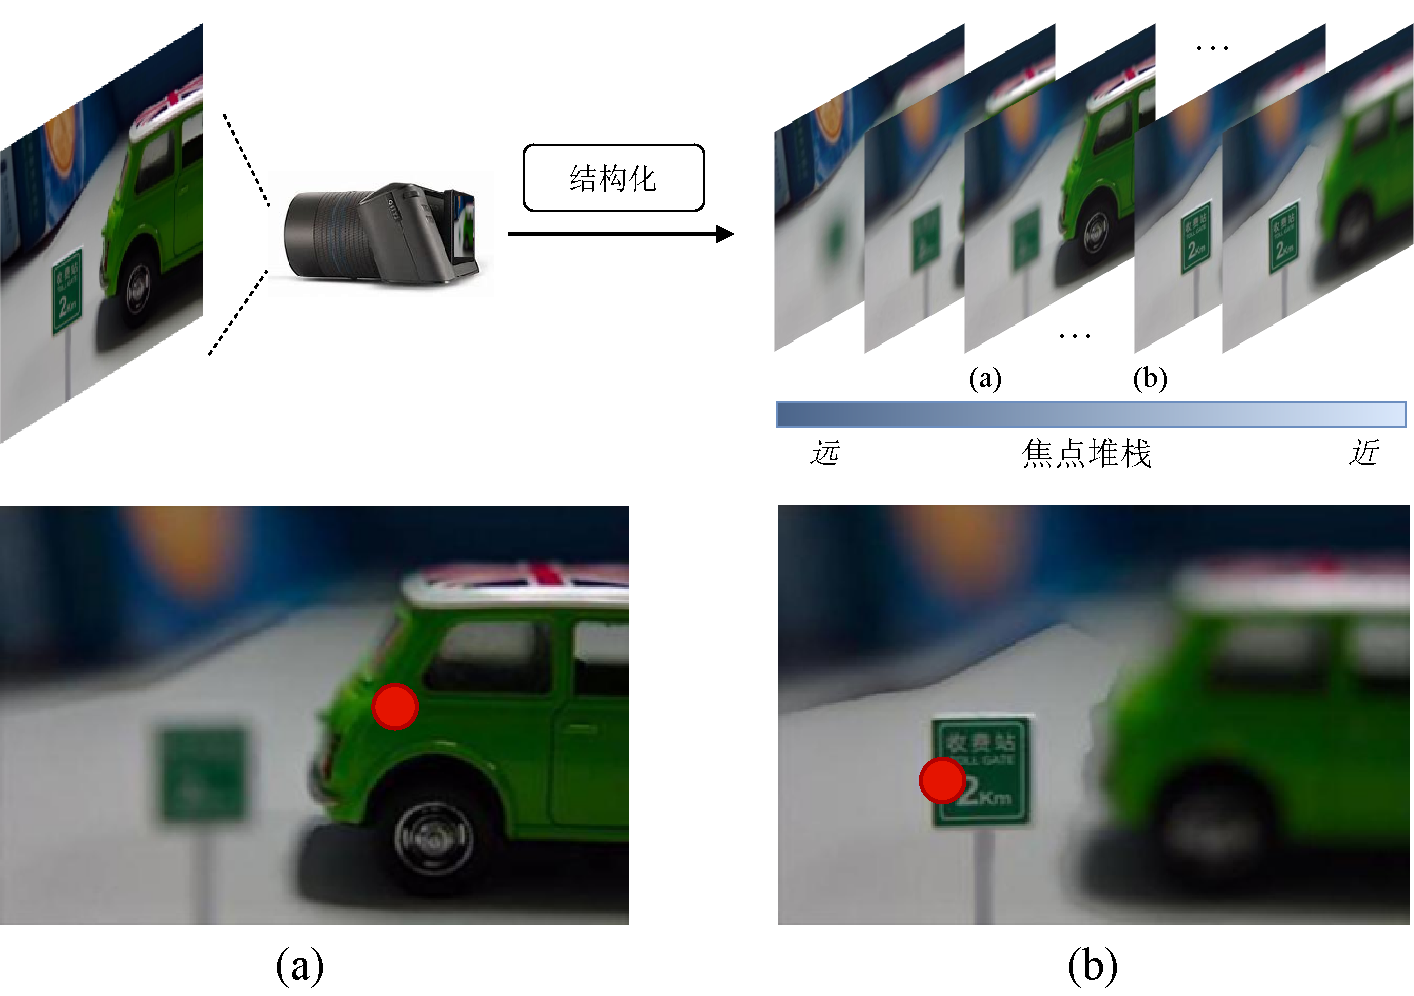
\includegraphics[width=0.85\linewidth]{figures/chapter3/cpt3_idea.pdf}
	\bicaption{光场焦点堆栈的成像过程和不同切片的成像效果}
	{The imaging process of the light field focus stack and the imaging effects of different slices}
	\label{figure:cpt3:idea}
\end{figure}




我们重新思考光场数据建模的方式。考虑到焦点堆栈的成像效果,如图~\ref{figure:cpt3:idea}~所示,每个焦点切片根据空间透视深度的不同,聚焦部位也不同。 并且从同一场景生成,焦点切片有很多共同点。
因此,即使在很小的带宽内,也可以充分总结和传达它们之间的差异。 此外,给定图像,人类可以毫不费力地关注敏感部分并忽略不重要的背景。 因此,在焦点堆栈中处理更多相对的焦点切片来模拟人类视觉系统是合理的。 


受上述观察的启发,我们考虑两个关键问题:
1)我们如何设计一个模型来存储切片级特征并在焦点堆栈和全焦点图像之间传递信息以进行上下文建模? 
2)我们如何设计一个模型来理解场景的空间分布并感知敏感的焦点切片? 

在本文中,我们提出了一种用于高效且有效的 LFSOD 的焦点感知Transformer(FPT)。 具体来说,我们收集图像特定的特征并制定通信以加强焦点堆栈和全焦点图像之间的相互感知。 我们利用选择性机制将适当的焦点切片纳入检测。 具体来说,我们的贡献有三个:



\begin{itemize}
	\item 我们引入与焦点相关的标记来总结图像特定的特征,并提出一种标记通信模块(TCM),通过计算与焦点相关的标记之间的交叉注意力来执行特征交互。 我们转移焦点堆栈中与焦点相关的标记以促进空间上下文传播。 
	
	\item 我们提出了一种焦点感知增强(FPE)策略,通过切片选择机制来增强焦点堆栈中的特征空间表示,以有区别地处理适当的焦点切片。	这可以突出显着切片并抑制非显着区域的干扰。 
	
	\item 我们对 4 个广泛使用的数据集进行了广泛的实验,并证明我们的方法优于现有最先进的 LFSOD 方法。 我们的方法在 DUTLF-FS~\cite{zhang2019memory}~上将 MAE 指标显着降低了 31\%。
\end{itemize}







%%%%%%%%%%%%%%%%%%%%%%%%%%%%%%%%%%%%%%%%%%%%%%%%%%%%%%%%%%%%%%%%%%%%%%%%%%%%%%
\BiSection{方法介绍}{Method Introduction}
%
%
%
%
%\par
\begin{figure}[!ht]
	\centering
	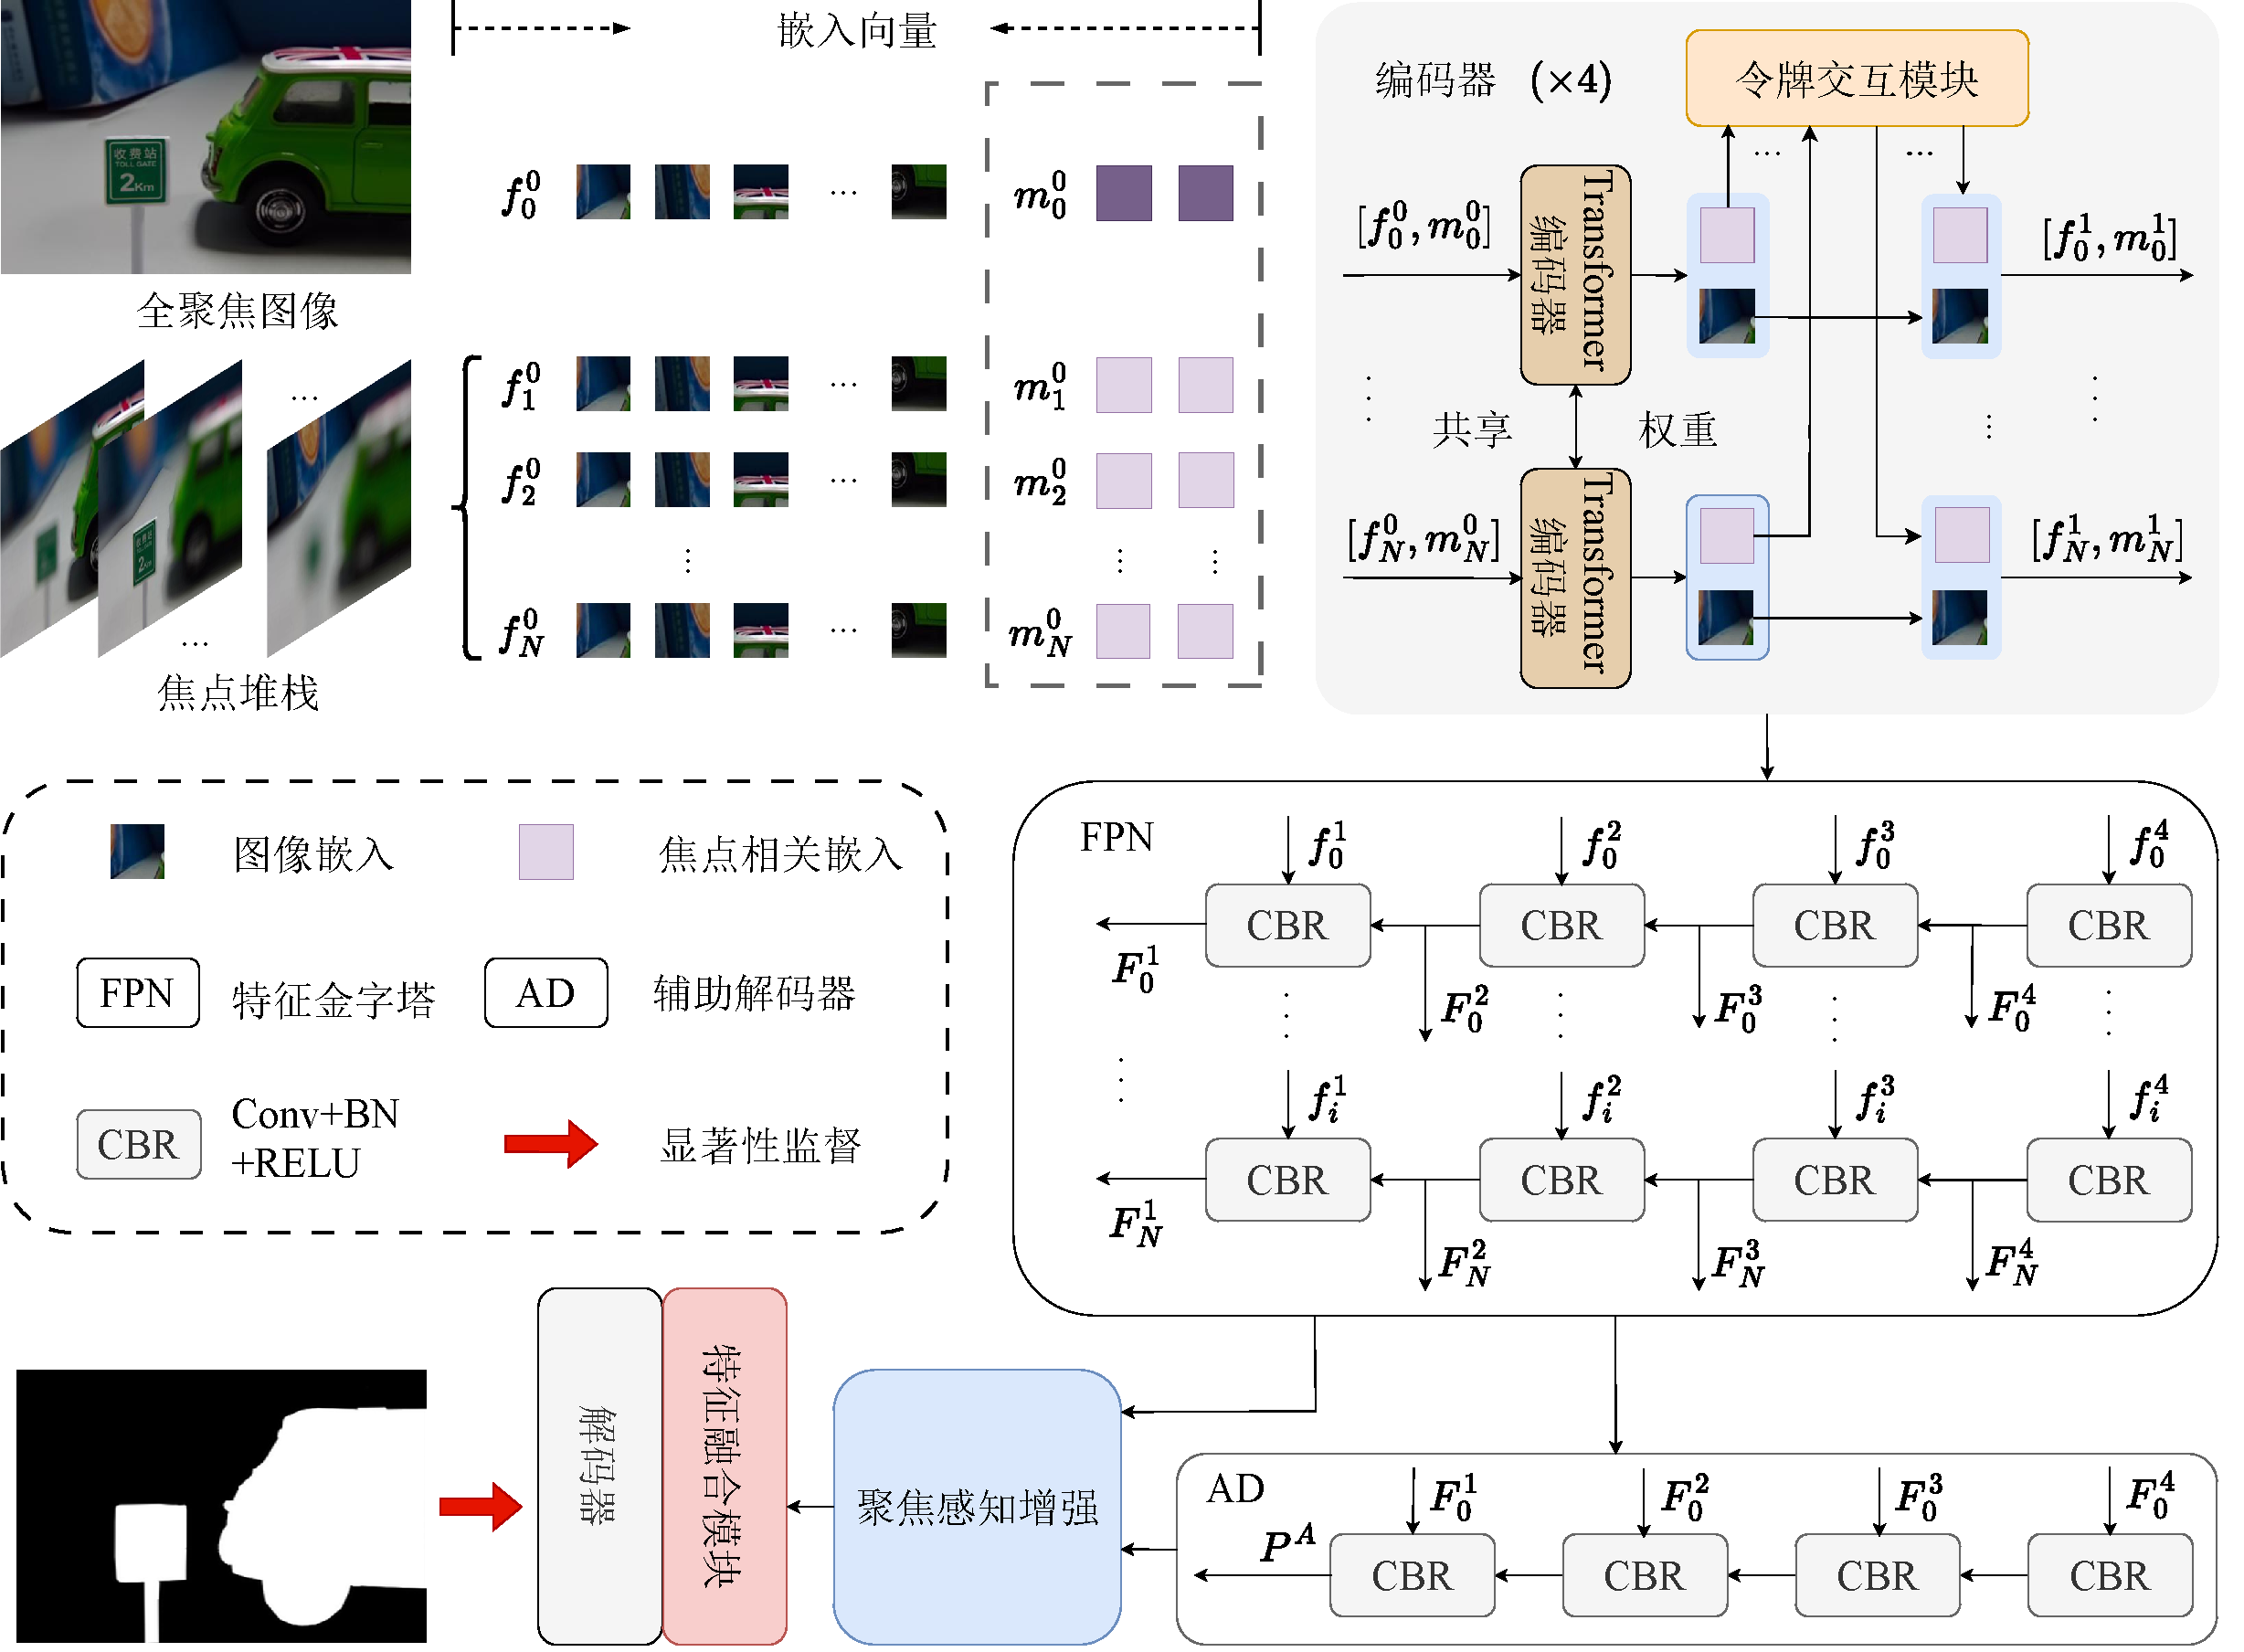
\includegraphics[width=0.95\linewidth]{figures/chapter3/overview_1}
	\bicaption{
		光场显著性目标检测网络的架构
	}{
		The architecture of light field salient object detection network
	}  
	\label{cpt3_fig1:overview}
\end{figure}
%
%
%
%
%
我们提出的 FPT 的整体架构如图 2 所示。给定 $N + 1$ 个分辨率为 $ H \times W $ 的图像,包括一个全焦点图像和 $N$ 个焦点堆栈图像,我们将每个图像划分为补丁区块作为输入。 
将展平的 $N$ 个 patch 输入到线性投影中,得到嵌入的 patch $ \left \{ f_{i}^{0} \right \}_{i=0}^{N} $,其形状为$ \left ( N + 1 \right ) \times \frac{HW}{P^{2}} \times C  $,其中 $P$ 表示每个 patch 的大小,$C$ 表示每个 patch 的大小。 
渠道维度。 
%
%
%
具体地,$ f_{0}^{0} $ 表示全焦点图像的特征输入。 
$ \left \{ f_{i}^{0} \right \}_{i=1}^{N} $ 表示焦点堆栈的特征输入。 
此外,为了总结补丁中的信息,引入了一组大小为 $ M \times C $ 的随机初始化的可学习嵌入,作为 { }N 个焦点相关标记,表示为 $ \left \{ m_{i}^{0} \right \}_{i=0}^{N} $ ,其中 $M$ 表示焦点相关标记的数量。 
我们将每个 patch 与焦点相关的标记连接起来,
并得到 $ \left \{ \left [ f_{i}^{0},m_{i}^{0}  \right ]  \right \}_{i=0}^{N} $ 作为特征提取器的输入。 
%
%
%
%
%
\par
%
%
与卷积网络使用不同的卷积步长来获得多尺度特征图不同,
我们使用渐进收缩策略通过patch嵌入层来控制特征图的尺度。
我们用$ l \in 1..T $ 表示阶段编号。 
我们将第$l$个阶段补丁块大小表示为$P_{l}$,在第$l$阶段开始时,
我们首先均匀划分输入特征图
$F_{l-1} \in \mathbb{R}^{H_{l-1} \times W_{l-1} \times C_{l-1}}$
为
$ \frac{H_{l-1}W_{l-1}}{P_{l}^{2}} $
个补丁块。

然后,将每个补丁块展平并投影到$C_{l}$维度的嵌入表达。
在线性投影之后,嵌入补丁的形状可以看做是
$\frac{H_{l-1}}{P_{l}} \times \frac{W_{l-1}}{P_{l}} \times C_{l} $,
其中高度和宽度比输入小了$P_{l}$倍。
这样我们可以灵活调整每个阶段的特征图的尺度,
使得可以构建基于Transformer的特征金字塔。
%
%
%
%
第$l$阶段的Transformer编码器有 $ N_{i} \in [3,4,6,3] $ 个 Transformer 块。
%
%
%
%
%
%\par
\begin{figure}[!ht]
	\centering
	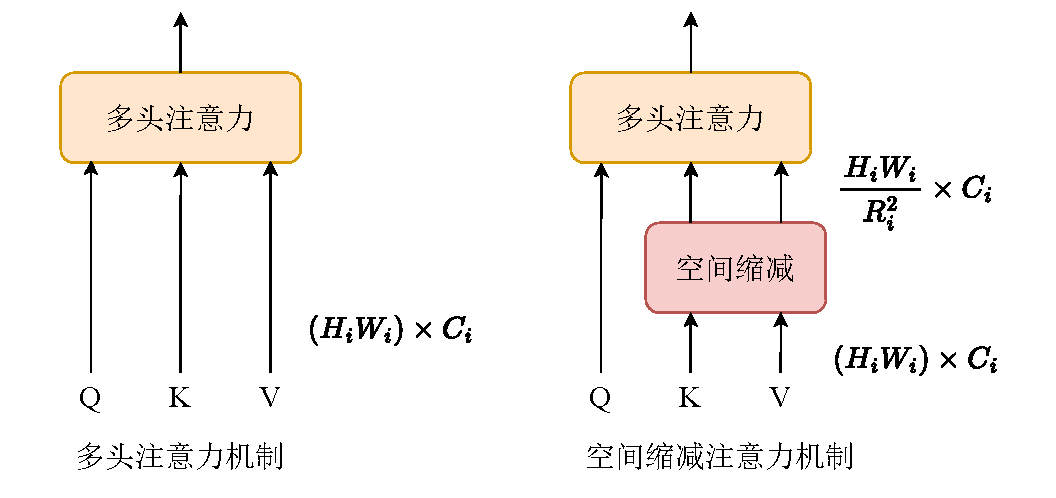
\includegraphics[width=0.95\linewidth]{figures/chapter3/sra}
	\bicaption{
		多头注意力与空间缩减注意力
	}{
		Multi-head attention (MHA) vs spatial reduction attention (SRA)
	}  
	\label{cpt3_fig1:sra}
\end{figure}
%
%
%
%
%
\par
%
%
我们构造基于金字塔Transformer(Pyramid Vision Transformer,PVT)~\cite{wang2022pvt}~的主干网由 $T = 4$ 个阶段组成。 
%
%~
%
由于骨干网络需要处理高分辨率的特征图,我们采用空间缩减注意力(Spatial-Reduction Attention,SRA)来取代Transformer编码器~\cite{vaswani2017attention}~中传统多头注意力(Multi-Head Attention)层。
%
%\\
%
%\\
%
\par 
%
%
与多头注意力机制类似,空间缩减注意力接受查询$Q$、秘钥$K$和值$V$作为输入,并细化输出的特征。
不同之处在于,仅需注意力操作之前缩减了$K$和$V$的空间尺度,如图~\ref{cpt3_fig1:sra},
能够在很大程度上减少计算和内存开销。
第$l$阶段的空间缩减注意细节可以表述如下:
%
%
%
%
\begin{equation}
	SRA(Q,~K,~V) = Concat(head_{0},~ \cdots,~ head_{H_{l}})~W^{O}
\end{equation}
%
%
\begin{equation}
	head_{j} = Attention(Q~W_{j}^{Q}, ~ SR(K)~W_{j}^{K},~ SR(V)~W_{j}^{V})
\end{equation}
%
%
%
其中$Concat(\cdot)$是连接操作。
$W_{j}^{Q} \in \mathbb{R}^{C_{i} \times d_{head}},~
W_{j}^{K} \in \mathbb{R}^{C_{i} \times d_{head}},~
W_{j}^{V} \in \mathbb{R}^{C_{i} \times d_{head}},~$
和
$W^{O} \in \mathbb{R}^{C_{i} \times C_{i}}~$
是线性映射参数。
$H_{l}$是每个阶段注意力层的头数。
$SR(\cdot)$是减少输入序列空间维度的操作,它的公式是:
%
%
%\\
%
\begin{equation}
	SR(x) = Norm(Reshape(x, R_{l})W^{S})
\end{equation}
%
%
其中$x \in \mathbb{R}^{(H_{l}W_{l}) \times C_{l}} $
表示输入序列,$R_{l}$表示每个阶段中的注意力层的缩减比例。
$Reshape(x, R_{l})$ 表示将输入序列 $x$ 重塑大小为
$\frac{H_{l}W_{l}}{R_{i}^{2}} \times (R_{i}^{2}C_{i})$。
$W_{S} \in \mathbb{R}^{R_{i}^{2}C_{i}}$
是一个线性投影,它将输入序列的维度减少到$C_{l}$。
$Norm(\cdot)$指的是层归一化。
%
%
\par
%
%
与原始的Transformer~\cite{vaswani2017attention}~中一样,
我们的每个 Transformer 块包括线性空间减少注意力 (SRA) 和前馈网络 (FFN),
以每个图像的方式作用于联合注意学习:
%%
%%
\begin{equation}
	\left \{ [f_{i}^{l}, m_{i}^{l}]\right \}_{i=0}^{N} = \left \{ FFN^{l} \left  ( SRA^{l} \left ( [f_{i}^{l-1}, m_{i}^{l-1}]\right )\right )\right \}_{i=0}^{N},
\end{equation}
%%
%%
每个Transformer编码器后面都布置了令牌通信模块(TCM),用于特征通信。 
%
%
%
%
%
%
%
%
%
%
%
%
%
%
\par
经过特征提取,我们从 Transformer 块的输出中得到四层特征 
$\left \{ f_{i}^{1},f_{i}^{2},f_{i}^{3},f_{i}^{4} \right \}_{i=0}^{N}$ 。 
之后,采用共享权重特征金字塔网络(FPN)~\cite{lin2017feature}~进行分层融合并得到 $N$ 个金字塔特征图	$ \left \{F_{i}^{1},F_{i}^{2},F_{i}^{3},F_{i}^{4} \right \}_{i=0}^{N}$:
%%
%%
\begin{equation}
	\begin{aligned}
		F_{i}^{4} &= Up \left ( CBR \left ( f_{i}^{4} \right )\right ) \\ 
		F_{i}^{l} &= Up \left ( CBR \left ( f_{i}^{l} + F_{i}^{l+1} \right )  \right ),l=1,2,3  .
	\end{aligned}
\end{equation}
%%
%%
其中 $Up$ 贡献 $2 \times $ 上采样 操作时,$CBR$ 表示一个卷积块,包括 Conv+ BN+ RELU 层。 对于解码器,提出的焦点感知增强(FPE)策略增强了焦点堆栈的特征表示。 增强的焦点堆栈和全焦点特征融合在特征融合模块(FFM)中。 最后,采用掩模解码器来生成显着图。

















%%%%%%%%%%%%%%%%%%%%%%%%%%%%%%%%%%%%%%%%%%%%%%%%%%%%%%%%%%%%%%%%%%%%%%%%%%%%%%
\BiSubsection{令牌交互模块}{Token Interaction Module}
%
%
%
%
%
%\par
\begin{figure}[!ht]
	\centering
	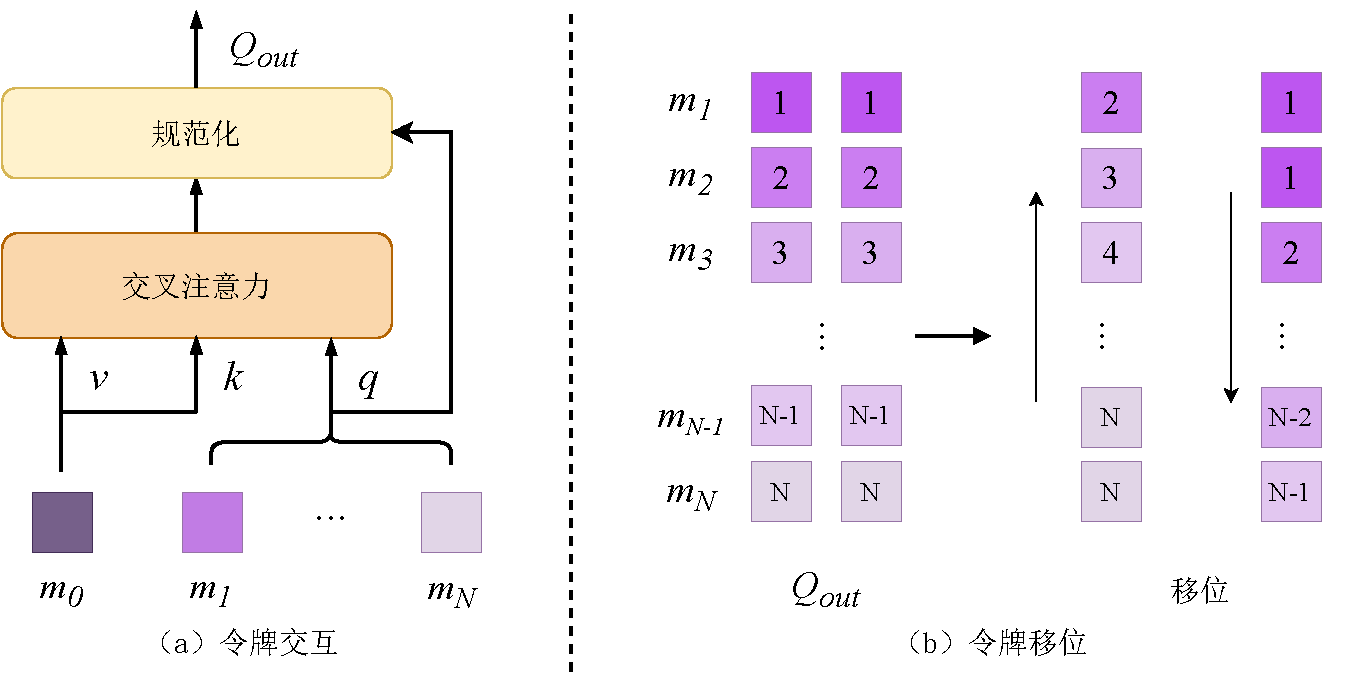
\includegraphics[width=0.95\linewidth]{figures/chapter3/token-interaction.drawio}
	\bicaption{
		令牌通信模块
	}{
		An illustration of the Token Communication Module (TCM)
	}  
	\label{cpt3_fig1:token_interaction}
\end{figure}
%
%
%
%
在以前的光场显著性检测方法中,主干网络仅以原像方式执行特征提取~\cite{piao2020exploit, liu2021light},忽略了光场数据固有的丰富上下文信息。 相比之下,我们设计了一个令牌通信模块(Token Communication Module,TCM)来对全焦点和焦点堆栈进行上下文建模,如图~\ref{cpt3_fig1:token_interaction}~所示。
TCM 由令牌交互(Token Interaction,TI)和令牌移位(Token Shift,TS)操作组成。 
令牌交互模块在全焦点和焦点堆栈的焦点相关令牌之间进行交叉注意力计算,以进行信息交互。 
令牌移位操作通过转移焦点堆栈中与焦点相关的标记,以促进上下文特征感知。 
%
%
%
%
%
\par
\textbf{令牌交互:}
如图~\ref{cpt3_fig1:token_interaction}~(a)~所示,令牌交互由交叉注意力 (Cross Attention,CA) 块组成。 
注意力函数可以描述为将查询和一组键值对映射到计算为值的加权和的输出。 
分配给每个值的权重是查询与相应键之间的相似度。 
这里,我们采用带有残差连接和层归一化的缩放点积注意力来实现交叉注意力块,公式可以表述如下:
%\todo
%
%
%
%%
\begin{equation}
	Attention(Q,K,V) = softmax \left ( \frac{QK^{T}}{\sqrt{d_{k}}} \right ) V,
\end{equation}
%%
%%
%
%
其中
$ Q \in \mathbb{R}^{N_{q}\times d_{k}}  $,
$ K \in \mathbb{R}^{N_{k}\times d_{k}}  $ 和
$ V \in \mathbb{R}^{N_{v}\times d_{k}}  $ 
分别是查询、键和值。 
$ d_{k} $ 是查询和密钥的通道维度,
$ \sqrt{d_{k}} $ 是控制softmax分布的温度参数。 
对于交叉注意力块,$K$ 和 $V$ 是相同的。 
%
%
%
%
%
\par
%
%
%
%
交叉注意力块将所有与焦点相关的标记 $ \left \{ m_{i}^{l} \right \}_{i=0}^{N} $ 作为输入。 焦点堆栈流的标记 $ \left \{  m_{i}^{l} \right \}_{i=1}^{N} $ 用作查询来计算与属于全焦点流的键 $ m_{0}^{l} $ 的相似度并从值 $ m_{0}^{l} $ 检索焦点信息。 该交叉注意力块的输出 $ Q_{out}^{l} $ 可计算如下:
%
%
%%
%%
\begin{equation}
	Q_{out}^{1} = LN \left ( Attention(Q,K,V) + Q \right ),
\end{equation}
%%
%%
%
%
其中
$ Q = \left \{ m_{i}^{1} \right \}_{i=1}^{N}~ W^{Q}$,
$ K= m_{0}^{1} ~W^{K} $,
$ V =  m_{0}^{1}~ W^{V} $。
$ Q$,$K$,$V$ 和 $ Q_{out}^{l} $
的维度分别为 
$ N \times M \times C $,$ M \times C $,$ M \times C $ 
和
 $ N \times M \times C $。 
%
%
%\\
%
\par
%
%
%
\textbf{令牌移位:}
%
%
上述操作的输出 $ Q_{out}^{l} $ 被馈送到令牌移位操作中,
如图~\ref{cpt3_fig1:token_interaction}~(b)~中所示。 
与焦点相关的标记被分为 $G = 2$ 组,并沿着焦点深度轴以不同方向(向前或向后)移动。 
对于每组焦点相关嵌入表示,可以看做是整体往左(或右)移动了一个图像级切片的位置。
经过一次移位操作,
每一张切片所对应的焦点相关嵌入由其左右两张切片的焦点相关嵌入的共同组合,
而对于两端的散焦切片,只汇总了一个方向上的不同图片的焦点相关嵌入信息。
%
%
%
%\\
%
%
\par
%
%
通过不同的焦点深度和方向,令牌可以实现与近深度和远深度焦点图像的空间特征进行上下文交换。 
然后我们用连接的 $ \left \{ m_{i}^{l} \right \}_{i=0}^{N} $ 更新所有与焦点相关的标记  $ \left \{ m_{i}^{l} \right \}_{i=0}^{N} $ 并将 
$ Q_{out}^{l} $ 移出。 
%
%
%\\
%
%
%\par
%
%
这种设计的目的是随着网络的深入,能够促进网络对于光场三维场景的整体感知,
从而保持稳定的空间感受野。 
值得一提的是,令牌移位操作几乎是无参数的,带来的计算成本可以忽略不计。







%%%%%%%%%%%%%%%%%%%%%%%%%%%%%%%%%%%%%%%%%%%%%%%%%%%%%%%%%%%%%%%%%%%%%%%%%%%%%%
\BiSubsection{聚焦感知增强策略}{Focus Perception Enhancement Strategy}
%
%
%
%
受人类视觉注意系统中关注选择性的启发,我们的目标是从多焦点特征中有效地感知有用的显着性信息。 我们提出了一种焦点感知增强(Focus Perception Enhancement,FPE)策略来模仿人类如何从视觉资源中选择感兴趣信息的筛选阶段。 
聚焦感知增强模块由切片选择机制组成,
用于有区别地处理焦点相关切片,
如图~\ref{cpt3_fig1:fpe}~所示。
选择机制可以突出显着切片并抑制非显着区域的干扰。 
此外,我们采用结构相似性~\cite{wang2003multiscale}~来评估焦点切片和全焦点图像之间焦点的一致性,
因为散焦状态下的物体不具有清晰的纹理结构。 
%
%
%
%
%\par
\begin{figure}[!ht]
	\centering
	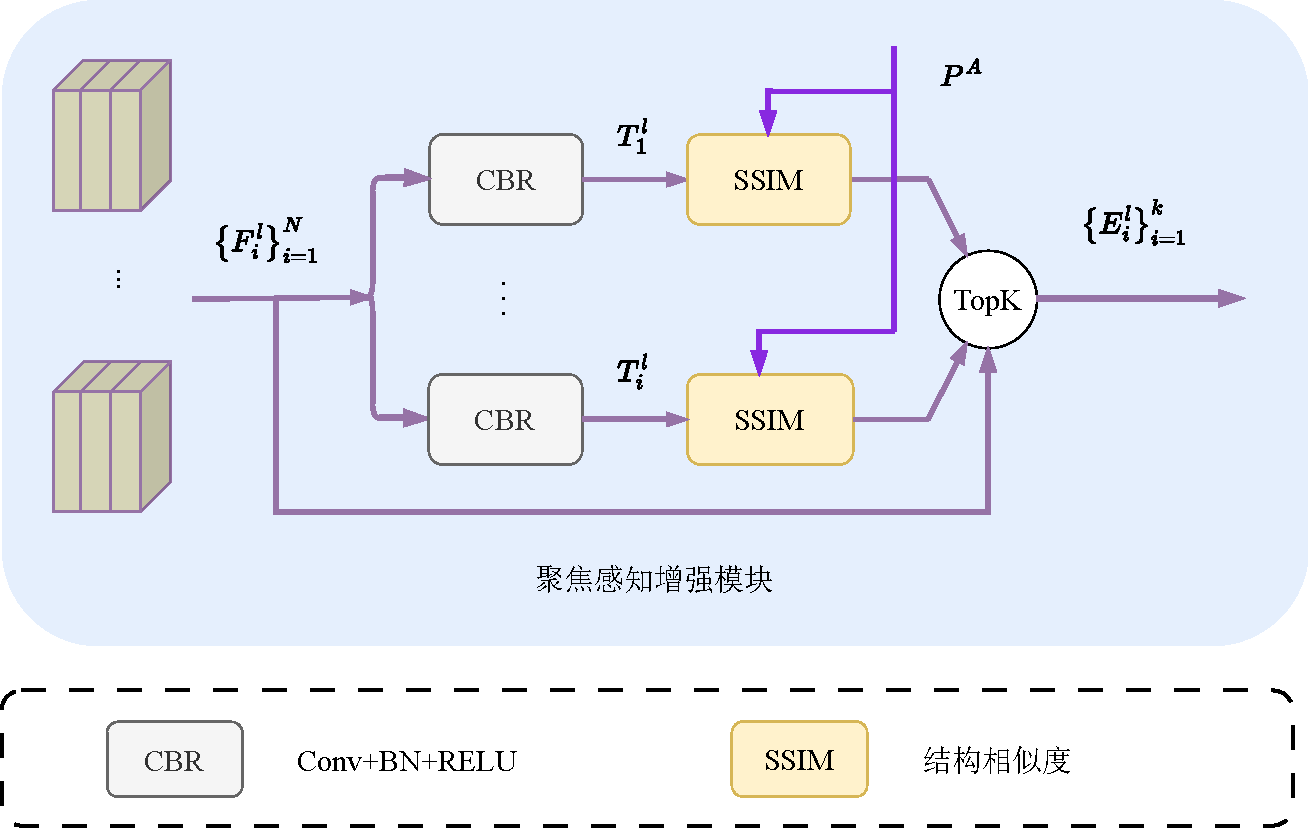
\includegraphics[width=0.90\linewidth]{figures/chapter3/fpe}
	\bicaption{
		聚焦感知增强模块
	}{
		Focused perception enhancement module
	}  
	\label{cpt3_fig1:fpe}
\end{figure}
%
%
%
%
\par
%
%
首先,我们使用基于特征金字塔网络的辅助解码器(Auxiliary Decoder,AD)生成辅助显着性预测 $ P^{A} $ 并应用监督以避免非显着对象的干扰并确保全焦点特征的有效性。 然后,我们使用全焦点显着性预测 $ P^{A} $ 计算焦点堆栈 $ \left \{ F_{i}^{l} \right \}_{i=1}^{N} $ 的每个层特征的结构相似度得分。 
%%
%%
\begin{equation}
	score_{i}^{l} = SSIM \left ( CBR \left ( F_{i}^{l} \right ), P^{A} \right ),
\end{equation}
%%
%%
%
%
其中 $CBR$ 表示一个卷积块,它将特征通道压缩成一维。 $SSIM$ 表示结构相似度,可以表示为: 
%
%
%%
%%
\begin{equation} 	
	SSIM(x,y)=\frac{\left ( 2\mu_{x}\mu_{y}+C_{1} \right ) \left (  2\sigma_{xy}+C_{2} \right )  } 	
	{\left ( \mu_{x}^{2} + \mu_{y}^{2}+C_{1}\right ) \left ( \sigma_{x}^{2}+ \sigma_{y}^{2} + C_{2} \right ) } , 	
\end{equation}
%%
%%
其中 $x$ 和 $y$ 表示两个输入图像,$\mu_{x}$、$\mu_{y}$ 和 $\sigma_{x}$ , $\sigma_{y}$分别是$x$和$y$的均值和标准差,$\sigma_{xy}$是它们的协方差,$C_{1} = 0.012$ 并且 $C_{2} = 0.032$ 用于避免被零除。 
%
%
%
%
\par
%
%
生成 $ score_{i}^{l} $ 后,我们选择前 $k$ 个对应的特征作为增强数据:
其中 $ TopK $ 是一种选择机制,在不改变原始空间顺序的情况下,根据 $ score_{i}^{l} $ 选择 $k$ 个最大值。 
%%
%%
\begin{equation}
	\left \{ E_{i}^{l} \right \}_{i=1}^{K} = TopK \left ( \left \{ score_{i}^{l}, F_{i}^{l} \right \}_{i=1}^{N} \right ), 	
\end{equation}
%%
%%
%
%
这种选择性焦点感知增强策略强调显着特征,同时抑制不必要的特征,这对于准确的显着目标检测至关重要。
%
%
%
%
\par
%
%
在获得增强的焦点堆栈和全焦点特征后,逐步设计特征融合模块(Feature Fusion Module,FFM)来融合特征,
如图~\ref{cpt3_fig1:ccm}~所示。
与全聚焦图的特征相比,焦点堆栈特征通常具有更高的数据维度, 一般为12倍大。 
因此,平衡差异化的数据维度可以被认为是特征函数的前提任务。
一些简单的解决方案直接连接高维特征并使用 2D 卷积来压缩特征~\cite{piao2021panet}~
或对每个焦点切片特征采用逐元素方式添加到融合数据\cite{liu2021light}。 然而,这些方法可能会阻止它们完全提取空间上下文信息,因为焦点堆栈在空间维度上是对齐的。 换句话说,生成的低维焦点堆栈特征无法提供足够的指导来实现高预测精度。 
%
%
%
%
%
%\par
\begin{figure}[!ht]
	\centering
	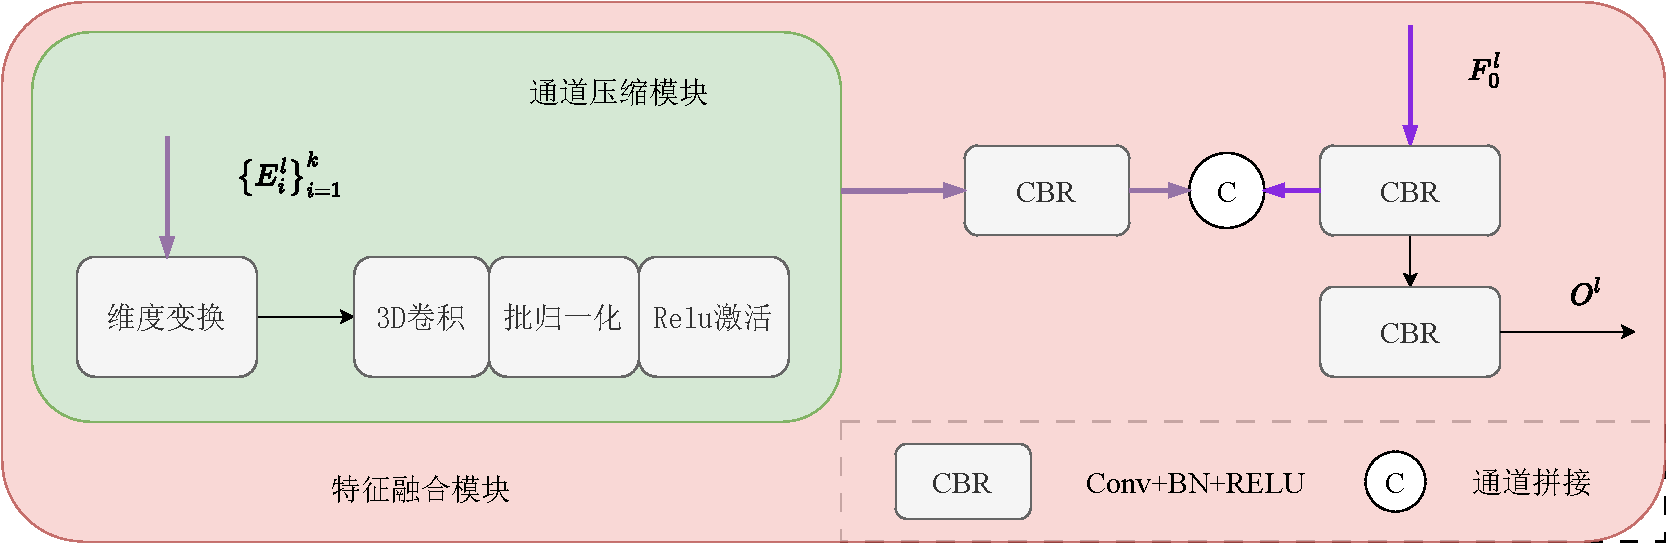
\includegraphics[width=0.95\linewidth]{figures/chapter3/ccm}
	\bicaption{
		特征融合模块
	}{
		Feature fusion module
	}  
	\label{cpt3_fig1:ccm}
\end{figure}
%
%
%
\par
%
%
我们提出了一种基于 3D 卷积的通道压缩模块 (Channel Compression Module,CCM) 来解决这个问题。 
通道压缩模块引入了3D卷积,它可以本质上提取时空特征来融合所有焦点堆栈特征。
具体来说,对于形状为 $ k \times C \times h \times w $ 的每一层增强焦点堆栈特征,
我们将其重塑为 $ C \times  k \times  h \times w $ ,然后使用内核为 $ k \times 1 \times 1 $  的 3D 卷积来融合空间上下文特征并压缩通道。 压缩特征 $ C^{l} $ 可以表示为:
%
%
%%
%%
\begin{equation}
	C^{l} = CCM \left ( Reshape \left ( E_{1-k}^{l} \right ) \right ) ,
\end{equation}
%%
%%
%
%
其中通道压缩模块主要由3D卷积组成,包括 $3DConv+BN+RELU$。 给定与输入形状相同的焦点堆栈和全焦点特征,采用多个卷积块进行跨域融合。 因此,我们将特征融合模块表述如下:
%
%
%	
%%
\begin{equation}
	%%
	O^{l}=CBR_{2}\left (Cat \left (CBR_{1} \left (F_{0}^{l} \right ),CBR_{1} \left (C^{l} \right ) \right ) \right ),
\end{equation}
%%
%%
%
%
其中 $CBR_{1}$ 和 $CBR_{2}$ 表示卷积块,包括 $Conv+BN+RELU$,前者使用 $1 \times C$ 通道输入,后者使用 $2 \times C$通道输入。
得到四层输出特征 $\left \{ O^{l} \right \}_{l=1}^{4} $ 后, 基于 FPN 的解码器~\cite{lin2017feature}~生成四个显着性预测图。 
其中最后一张用作最终的显着性预测图。 
%
%
%
%
%
%\BiSubsection{损失函数}{TODO}








%%%%%%%%%%%%%%%%%%%%%%%%%%%%%%%%%%%%%%%%%%%%%%%%%%%%%%%%%%%%%%%%%%%%%%%%%%%%%%
\BiSubsection{训练过程}{Training Process}
%
%
本文所提出的网络模型使用一个混合损失函数来训练。
%
%
二元交叉熵(Binary Cross Entropy,BCE)~\cite{de2005tutorial}~是二元分类和分割中使用最广泛的损失函数。 但 $\mathcal L_{bce} $ 是像素级损失,这意味着它平等对待所有像素。
在具有主导背景的图片中,前景像素的损失将会被稀释。 最近,显著性网络~\cite{qin2019basnet}~中引入了交并比(Intersection over Union,IoU)损失来弥补二元交叉熵损失的不足。
$ \mathcal L_{iou} $ 的目标是优化全局结构,而不是专注于单个像素,这样就不会受到分布不平衡的影响。 增强对齐度量~\cite{fan2018enhanced}~首先被提出作为一种可以同时考虑像素级和图像级误差的评估指标,
损失形式为 $ \mathcal L_{em} = 1 - E_{\xi} $。 

%
%
%
%
%
%
基于上述讨论,我们构建了一个混合损失:
%
%
%
%%
\begin{equation} 
	% L = L_{BCE} \left (  P,G \right )  + L_{IOU} \left ( P,G  \right ) + L_{EM} \left ( P,G  \right ) 
	\mathcal L = \mathcal L_{bce} + \mathcal L_{iou}  + \mathcal L_{em}  .
\end{equation}
%
%
%
%
\par
%
%
如图~\ref{cpt3_fig1:overview}~所示,我们的模型有两个掩码头,它们预测辅助显着性图 $ P^{A} $ 和四个最终多尺度显着性图 $ \left \{ P_{i}^{S} \right \}_{i=1}^{4} $ 。 因此,所提出的网络的总损失 $ \mathcal L_{total} $ 可以表示为: 
%
%% 
%%
%%
\begin{equation}
	\mathcal L_{total} = \mathcal L\left ( P^{A}, G \right ) + \lambda  \sum_{i=1}^{4} \left ( \mathcal L \left (  P_{i}^{S},G \right )\right ),
	%% \mathcal L_{total} = \mathcal L\left ( T_{0}, G \right ) + \lambda  \sum_{i=0}^{3} \left ( \mathcal L \left (  P_{i}^{S},G \right )\right )
	%% \mathcal L_{total} = \mathcal L\left ( T_{0}, G \right ) + \lambda  \sum_{i=0}^{3} \left ( \mathcal L \left (  P_{i},G \right )\right )
\end{equation}
%%
%%
%
%
%
其中 $ G $ 表示真值图。$ \mathcal L $代表我们用来逐渐优化预测的混合损失。 $ \lambda $是用于辅助控制监督项权重的超参数。




















%%%%%%%%%%%%%%%%%%%%%%%%%%%%%%%%%%%%%%%%%%%%%%%%%%%%%%%%%%%%%%%%%%%%%%%%%%%%%%
\BiSection{实验结果与分析}{Experimental Results and Analysis}

\BiSubsection{实验设置}{Experimental Setup}



%%%%%%%%%%%%%%%%%%%%%%%%%%%%%%%%%%%%%%%%%%%%%%%%%%%%%%%%%%%%%%%%%%%%%%%%%%%%%%
(1)实验数据集
%
%
\par
%
%
我们的实验是在四个公共光场基准数据集上进行的:LFSD~\cite{li2014saliency}、HFUT~\cite{zhang2017saliency}、DUTLF-FS~\cite{zhang2019memory}~和 DUTLF-V2~\cite{piao2020dut}。 HFUT 和 LFSD 相对较小,分别仅包含 255 个和 100 个样本。 DUTLF-V2是最大的数据集,包含4204个样本,分为2957个和1247个分别用于训练和测试。 DUTLF-FS包含1462个样本,分别分为1000个训练样本和462个测试样本。 每个样本都包含一个全焦点图像、几个焦点切片以及相应的真值显着性图。
%
%
%
%
\par
%
%
%
%------------------------------ figure: comparison
\begin{figure}[!ht]
	\centering
	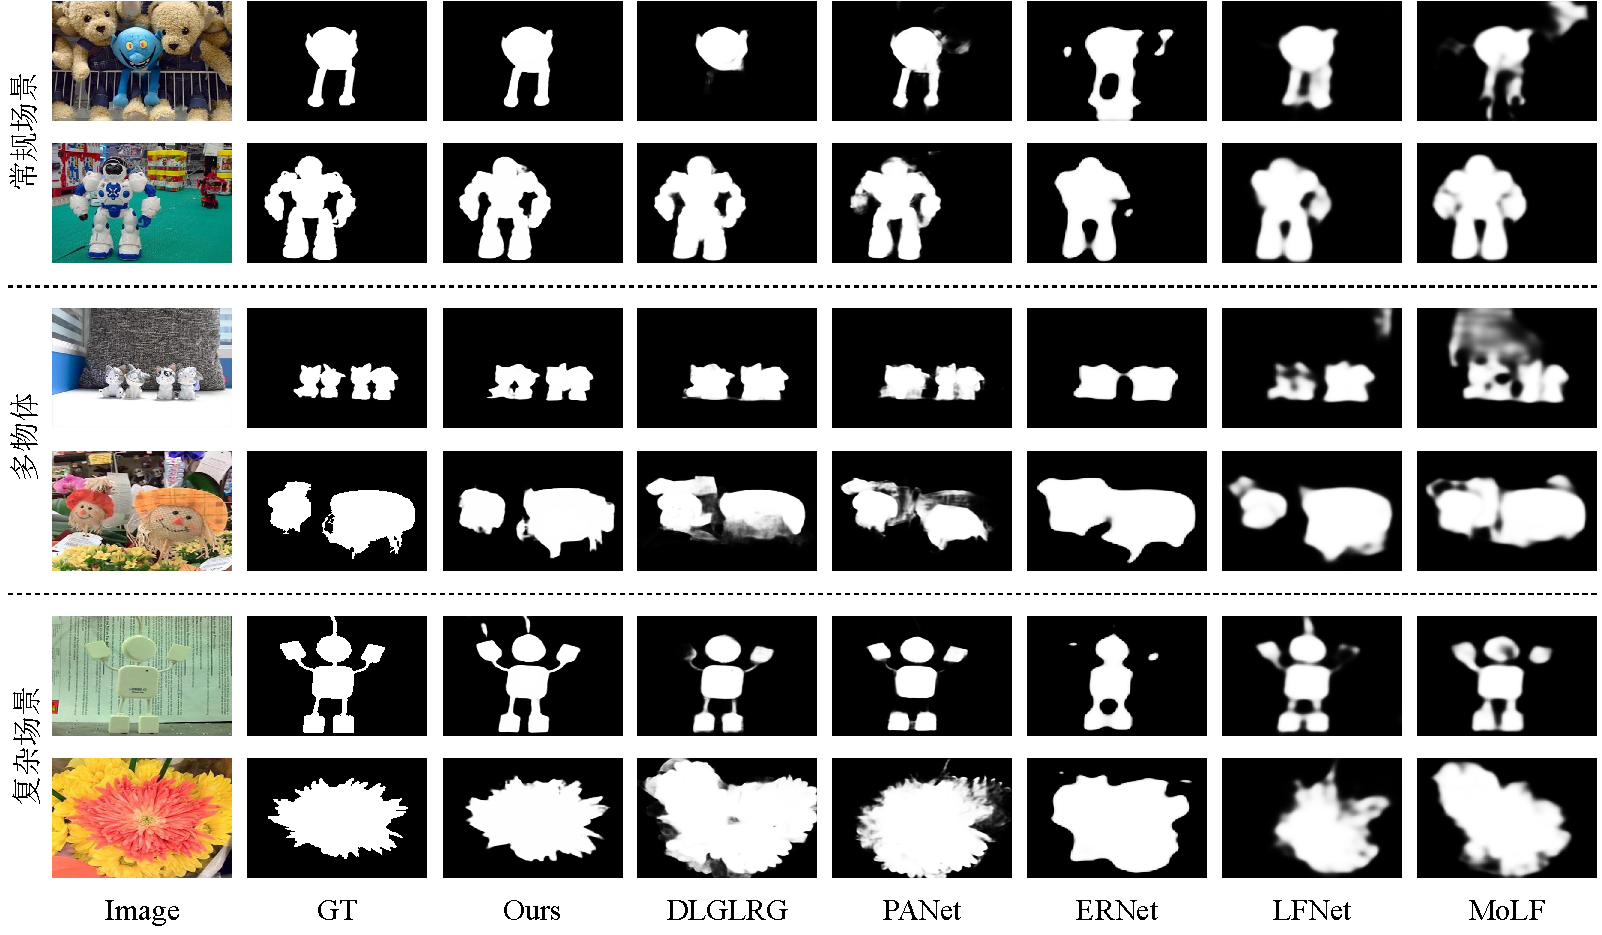
\includegraphics[width=\linewidth]{figures/chapter3/compare_1}
	\bicaption{
		在一些具有挑战性的场景中与最先进的方法的可视化比较
	}{
		Visual comparisons with state-of-the-art methods in challenging scenes
	}
	\label{figure:figure_comparison_1}
\end{figure}






%%%%%%%%%%%%%%%%%%%%%%%%%%%%%%%%%%%%%%%%%%%%%%%%%%%%%%%%%%%%%%%%%%%%%%%%%%%%%%
(2)实现细节
%
%
\par
%
%
为了公平比较,我们遵循大多数以前的方法~\cite{piao2020exploit, liu2021light}~使用 DUTLF-FS 和 HFUT 的训练集来训练我们的 FPT,以便与使用焦点堆栈输入训练的其他光场方法进行比较。 我们按照~\cite{wang2022lfbcnet,jing2021occlusion}~使用 DUTLF-V2 的训练集来训练我们的模型,以便与使用多视图输入训练的其他最先进的 LFSOD 方法进行比较。 我们将每个图像的大小调整为 $256 \times 256$,以便于在训练和测试中实现,并且我们还通过随机翻转、裁剪和旋转来增强训练数据。
我们使用预训练的 PVT-B2~\cite{wang2022pvt}~模型作为我们的主干,因为它具有与 ResNet50~\cite{he2016deep}~相似的计算复杂性。 我们共享全焦点和焦点堆栈模式之间的主干权重,以减少不必要的参数。 整个网络使用 Adam~\cite{kingma2014adam}~作为优化算法进行端到端训练,并将初始学习率设置为 1e-4。 小批量大小设置为 2,我们的网络训练了 80 个循环迭代。 学习率在第 40 和 70 个迭代循环时分别乘以 0.1。 所提出的方法是使用Pytorch工具箱~\cite{paszke2017automatic}~实现的,所有实验都在四个RTX 1080Ti GPU上进行。 我们的代码将可用。 
%
%
%
%
%
\par
%
%
%\\
%\\
%
%
%
(3)评价指标
%
%
\par
%
%
本章采用了绝对平均误差、S-measure、E-measure和F-measure作为评
估模型性能的指标。




%%%%%%%%%%%%%%%%%%%%%%%%%%%%%%%%%%%%%%%%%%%%%%%%%%%%%%%%%%%%%%%%%%%%%%%%
\BiSubsection{消融实验}{Ablation Experiment}



\begin{table}[!ht]
	\bicaption{	
		与多视图 LFSOD 方法比较的定量结果
	}{
		Quantitative results of comparison with multi-view LFSOD methods
	}
	\centering
	\label{chpt3:table:comp_sota}
	\resizebox{\linewidth}{!}{
		\begin{tabular}{rcccccccccccc}
			\toprule[2pt]  %添加表格头部粗线
			
			% title
			%			\multirow{2}*{Type} & 
			\multicolumn{1}{c}{ \multirow{2}*{方法} } & 
			\multicolumn{4}{c}{DUTLF-FS \cite{zhang2019memory} } &
			\multicolumn{4}{c}{HFUT \cite{zhang2017saliency} } &
			\multicolumn{4}{c}{LFSD \cite{li2014saliency} } \\
			
			% next line
			\cmidrule(r){2-5} \cmidrule(r){6-9} \cmidrule(r){10-13}
			
			%			 subtitle
			& $E_{\phi}^{max}\uparrow$ & $S_{\alpha }\uparrow$ & $F_{\beta}^{max}\uparrow$ & MAE$\downarrow$ 
			& $E_{\phi}^{max}\uparrow$ & $S_{\alpha }\uparrow$ & $F_{\beta}^{max}\uparrow$ & MAE$\downarrow$  
			& $E_{\phi}^{max}\uparrow$ & $S_{\alpha }\uparrow$ & $F_{\beta}^{max}\uparrow$ & MAE$\downarrow$ \\
			
			%			& E & S & F & MAE 
			%			& E & S & F & MAE 
			%			& E & S & F & MAE \\
			
			
			% line line
			\midrule[1pt]
			
			%			\multirow{8}*{\textit{Light field}}
			
			% 开始填数据
			
			Ours	 
			&  {\textbf{.973}} & \textbf{ {.946}} 	& \textbf{ {.954}} & \textbf{ {.020}} 
			& \textbf{ {.871}} &	\textbf{ {.828}} 			&\textbf{	 {.784}} & {\textcolor{red}{.064}} 
			& \textbf{ {.919}} &	\textcolor{blue}{.860} 			&	\textbf{ {.873}} &	\textbf{ {.064}} 
			\\
			
			DLGLRG \cite{liu2021light} 
			& {\textcolor{red}{.958}} & {\textcolor{red}{.928}} 			& {\textcolor{red}{.934}} & {\textcolor{red}{.029}} 
			&	.839 &	.766 &	.698 &	.070 
			&	{\textcolor{red}{.906}} &	\textbf{ {.866}} 			&	{\textcolor{red}{.870}} &	\textcolor{blue}{.069} 
			\\
			
			ERNet \cite{piao2020exploit}
			& .947 & .899 & .908 & .039 
			&	.841 &	.778 &	.722 &	.082 
			&	.888 &	.834 &	.850 &	.082 
			\\
			
			PANet \cite{piao2021panet} 
			& .939 & .908 & .903 & .038 
			& .845 & .795 & .738 & .074 
			& .892 & .849 & .849 & .076
			\\
			
			LFNet	 \cite{zhang2020lfnet} 
			& .929 & .878 & .890 & .053
			&	.846 &	.782 &	.718 &	.073 
			&	.885 &	.820 &	.824 &	.092 \\
			
			MAC	 \cite{zhang2020light} 
			& .863	& .804	& .792	& .102	
			&   .797 & .731 & .667 & .107 
			& .832 & .782 & .776 & .127 \\
			
			MoLF	 \cite{zhang2019memory} 
			& .938 & .887 & .902 & .051 
			&	.852 &	.789 &	.729 &	.075 
			&	.888 &	.830 &	.834 &	.089 \\
			
			DLSD	\cite{piao2019deep}
			& .891	& .841	& .801	& .076	
			&   .783 & .741 & .615 & .098 
			& .806 & .737 & .715 & .147 \\
			
			\midrule[1pt] % end lfsod
			
			% start rgb-d
			%			\multirow{6}*{\textit{RGB-D}}
			
			DCF \cite{ji2021calibrated} 
			& \textcolor{blue}{.954} & \textcolor{blue}{.921} & \textcolor{blue}{.927} & \textcolor{blue}{.031} 
			& \textcolor{blue}{.856} & {\textcolor{red}{.812}} & {\textcolor{red}{.768}} & \textcolor{blue}{.065} 
			& .881 & .809 & .821 & .096 \\
			
			CIR-Net \cite{cong2022cir}
			& .950 & .916 & .921 & .038 
			& {\textcolor{red}{.862}} & .800  			& .742 & \textbf{ {.062}} 
			& .874 & .820 & .816 & .098 \\ 
			
			VST-$rgbd$  \cite{liu2021visual} 
			& .952 & .920 & .921 & .036 
			& .843 & .807 & .754 & .086 
			& .851 & .792 & .786 & .110 
			\\
			
			%			& -  & 2022  & \\
			%			& -  & 2022  & \\
			
			BBS-Net     \cite{fan2020bbs} 
			& .900 & .865 & .852 & .066 
			& .801 & .751 & .676 & .073 
			& \textcolor{blue}{.901} & {\textcolor{red}{.864}} & .858 & .072 \\ 
			
			SSF     \cite{zhang2020select} 
			& .922 & .879 & .887 & .050 
			& .816 & .725 & .647 & .090 
			& \textcolor{blue}{.901} & .859 & \textcolor{blue}{.868} & {\textcolor{red}{.067}} \\ 
			
			S2MA    \cite{liu2020learning} 
			& .839 & .787 & .754 & 	.102 
			& .777 & .729 & .650 & .112 
			& .873 & .837 &	.835 & .094 \\
			
			
			\midrule[1pt] 
			
			%			\multirow{7}*{\textit{RGB}}
			
			VST-$rgb$ \cite{liu2021visual} 
			& .939 & .910 & .911 & .047
			& .831 & \textcolor{blue}{.808} & \textcolor{blue}{.763} & .093 
			& .865 & .797 & .817 & .123 
			\\ 
			
			PFSNet \cite{ma2021pyramidal}
			& .912 & .883 & .879 & .057 
			& .835 & .800 & .752 & .088 
			& .805 & .749 & .727 & .145 
			\\ 
			
			
			ITSD \cite{zhou2020interactive} 
			& .930 & .899 & .899 & .052 
			& .839 & .805 & .759 & .089 
			& .879 & .847 & .840 & .088 
			\\ 
			
			
			
			LDF \cite{wei2020label} 
			& .898 & .873 & .861 & .061 
			& .804 & .780 & .708 & .093 
			& .843 & .821 & .803 & .096 
			\\ 
			
			
			MINet \cite{pang2020multi} 
			& .916 & .890 & .882 & .050 
			& .816 & .792 & .720 & .086 
			& .861 & .834 & .828 & .091 
			\\ 
			
			F$^{3}$Net  \cite{wei2020f3net}
			& .900 & .888 & .882 & .057 
			& .815 & .777 & .718 & .095 
			& .824 & .806 & .797 & .106 
			\\ 
			
			
			EGNet   \cite{zhao2019egnet}
			& .914 & .886 & .870 & .053 
			& .794 & .772 & .672 & .094 
			& .776 & .784 & .762 & .118 
			\\ 
			
			CPD  \cite{wu2019cascaded}
			& .867 & .911 & .866 & .058 
			& .772 & .82  & .701 & .086 
			& .759 & .82  & .759 & .126 \\
			
			PoolNet \cite{liu2019simple}
			& .889 & .919 & .868 & .051 
			& .776 & .802 & .683 & .092 
			& .789 & .8   & .769 & .118 \\
			
			PiCANet \cite{liu2018picanet}
			& .829 & .892 & .821 & .083 
			& .726 & .781 & .618 & .115 
			& .729 & .78  & .671 & .158 \\
			
			PAGRN \cite{wang2018detect}
			& .822 & .878 & .828 & .084 
			& .717 & .773 & .635 & .114 
			& .727 & .805 & .725 & .147 \\
			
			C2S   \cite{li2018contour}
			& .844 & .874 & .791 & .084 
			& .763 & .786 & .65  & .111 
			& .806 & .82  & .749 & .113 \\
			
			R3Net  \cite{deng2018r3net}
			& .833 & .819 & .783 & .113 
			& .727 & .728 & .625 & .151 
			& .789 & .838 & .781 & .128 \\
			
			Amulet \cite{zhang2017amulet}
			& .847 & .882 & .805 & .030 
			& .767 & .76  & .636 & .110  
			& .773 & .821 & .757 & .135 \\
			
			
			\bottomrule[2pt] % end
		\end{tabular}
	}
	%	\vspace{3cm}
\end{table}



%---------------------------------------------------------------------> 消融实验: 多视角方法对比
%
\begin{table}[!hb]
	\bicaption{	
		与多视图 LFSOD 方法比较的定量结果
	}{
		Quantitative results of comparison with multi-view LFSOD methods
	}
	\centering
	\label{table:comp_multi_view}
	%	\resizebox{\linewidth}{!}{
		\begin{tabular}{crcccc}
			\toprule[2pt]  %添加表格头部粗线
			
			% title
			\multirow{2}*{输入类型} & \multicolumn{1}{c}{\multirow{2}*{方法}} & \multicolumn{4}{c}{DUTLF-V2 \cite{piao2020dut}} \\
			
			% next line
			\cmidrule(r){3-6} 
			
			% subtitle
			& & $E_{\phi}^{max}\uparrow$ & $S_{\alpha }\uparrow$ & $F_{\beta}^{max}\uparrow$ & MAE$\downarrow$ \\
			
			\midrule[1pt]  % E S F MAE
			
			焦点堆栈       & \multicolumn{1}{c}{ Ours$^{\ast} $ } &
			\textbf{ 0.960 } & \textbf{ 0.923 }  & \textbf{ 0.917 }  & \textbf{ 0.026 }  \\ 
			%								 &  0.9598 & 0.9227 & 0.9173 & 0.0256 \\
			% multiview
			
			\midrule[1pt]
			
			\multirow{3}*{多视角图}
			& OBGNet \cite{jing2021occlusion}      &  0.940  & 0.896  & 0.885  & 0.037  \\
			& LFBCNet \cite{wang2022lfbcnet}    &  0.940  & 0.890  & 0.870  & -      \\
			& ESCNet \cite{zhang2022exploring}      &  0.931  & 0.882  & 0.852  & 0.041  \\
			
			
			\bottomrule[2pt]
		\end{tabular}
		%}
\end{table}


%------------------------------ figure: comparison
\begin{figure}[!ht]
	\centering
	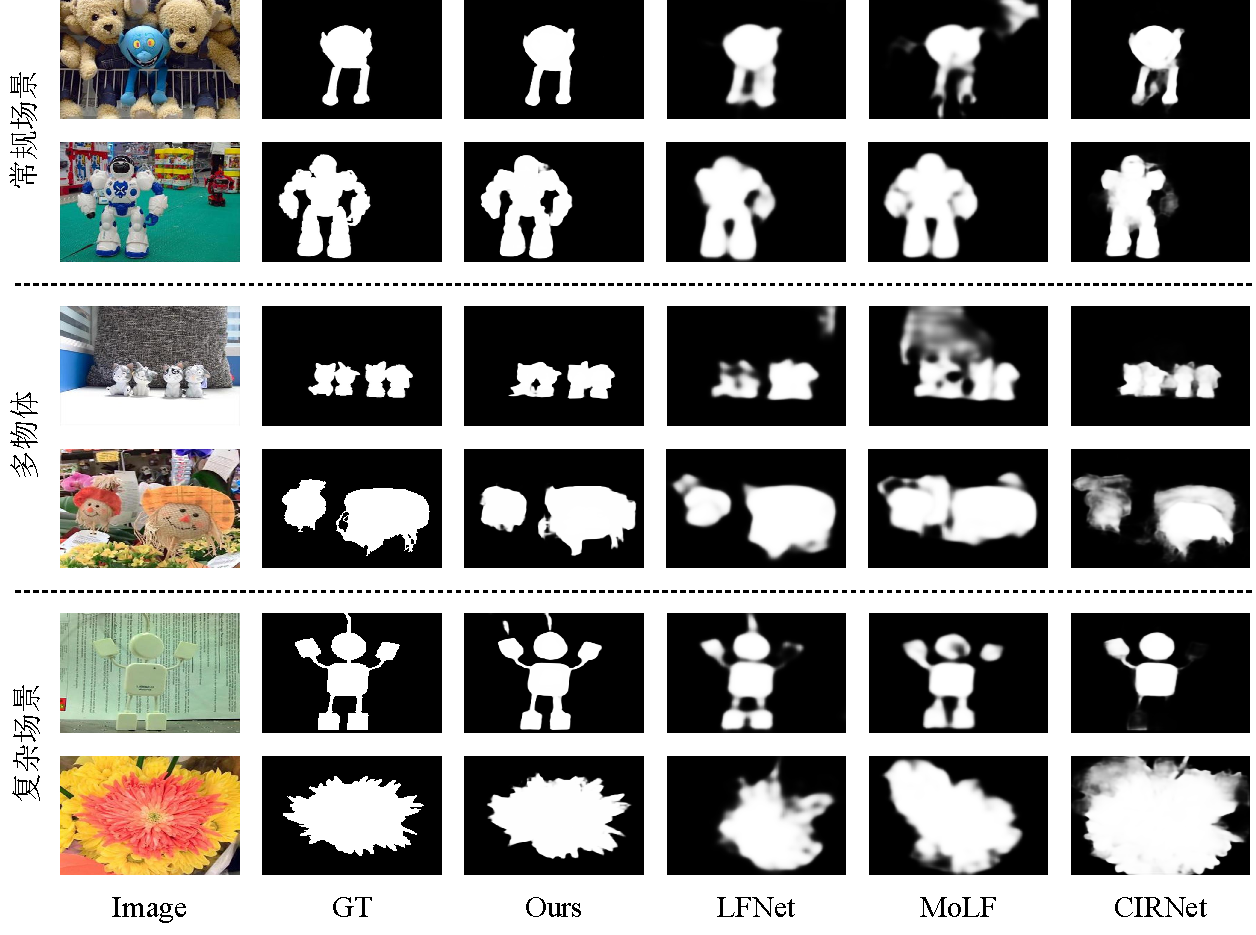
\includegraphics[width=\linewidth]{figures/chapter3/compare_2}
	\bicaption{在一些具有挑战性的场景中与最先进的方法的可视化比较}
	{Visual comparisons with state-of-the-art methods in challenging scenes}
	\label{figure:figure_comparison_2}
\end{figure}


%%%%%%%%%%%%%%%%%%%%%%%%%%%%%%%%%%%%%%%%%%
(1)定量比较

为了进行全面比较,我们将我们的方法与 26 个最先进的模型进行比较,
包括6个光场显著性分割方法:
DLGLRG \cite{liu2021light}, RENet \cite{piao2020exploit}, LFNet \cite{zhang2020lfnet},
MAC \cite{zhang2020light}, MoLF \cite{zhang2019memory}, and DLSD \cite{piao2019deep};
%
%
%
%
6个RGB-D显著性分割方法:
DCF \cite{ji2021calibrated}, CIR-Net \cite{cong2022cir}, VST-$rgbd$  \cite{liu2021visual},
BBS-Net     \cite{fan2020bbs}, SSF     \cite{zhang2020select} and S2MA    \cite{liu2020learning};
%
%
%
%
%
和14个2D显著性检测方法:
VST-$rgb$ \cite{liu2021visual},
PFSNet \cite{ma2021pyramidal},
ITSD \cite{zhou2020interactive},
LDF \cite{wei2020label},
MINet \cite{pang2020multi},
F$^{3}$Net  \cite{wei2020f3net}, 
EGNet   \cite{zhao2019egnet},
CPD  \cite{wu2019cascaded},
PoolNet \cite{liu2019simple},
PiCANet \cite{liu2018picanet},
PAGRN \cite{wang2018detect},
C2S   \cite{li2018contour},
R3Net  \cite{deng2018r3net}
和
Amulet \cite{zhang2017amulet}。






为了保证公平比较,我们使用他们提供的显着性预测图或预训练的权重来生成比较数据,
并利用~\cite{liu2021visual}~提供的相同评估代码。
如表~\ref{chpt3:table:comp_sota}~所示,
很明显,所提出的方法在 DUTLF-FS 和 HFUT 数据集上实现了比当前最先进的方法更优越的性能。 同时,所提出的方法可以在除了 $ S_{\alpha} $ 的另外三个指标上超越其他方法。 值得一提的是,与使用大量数据集训练的 RGBD 和 RGB 的显著性检测方法相比,我们的方法在小三倍的训练集(1100 vs. 2985 vs. 10553)下取得了显着的优势。 这表明我们的方法可以有效地探索光场数据中传达的信息。 


我们还在 DUTLF-V2 上重新训练我们的方法,并与其他三种使用多视图图像作为输入的光场显著性目标分割方法进行比较,
包括 OBGNet ~\cite{jing2021occlusion}、LFBCNet~\cite{wang2022lfbcnet}~ 和 ESCNet~\cite{zhang2022exploring}。 如表~\ref{table:comp_multi_view}~所示,我们的方法可以在 DUTLF-V2 的所有四个指标上大幅实现最佳性能。 这证明了我们网络对于使用焦点堆栈作为输入的有效性以及信息提取的高效性。 



%---------------------------------------------------------------------> figure: overview 
\begin{figure}[t] 
	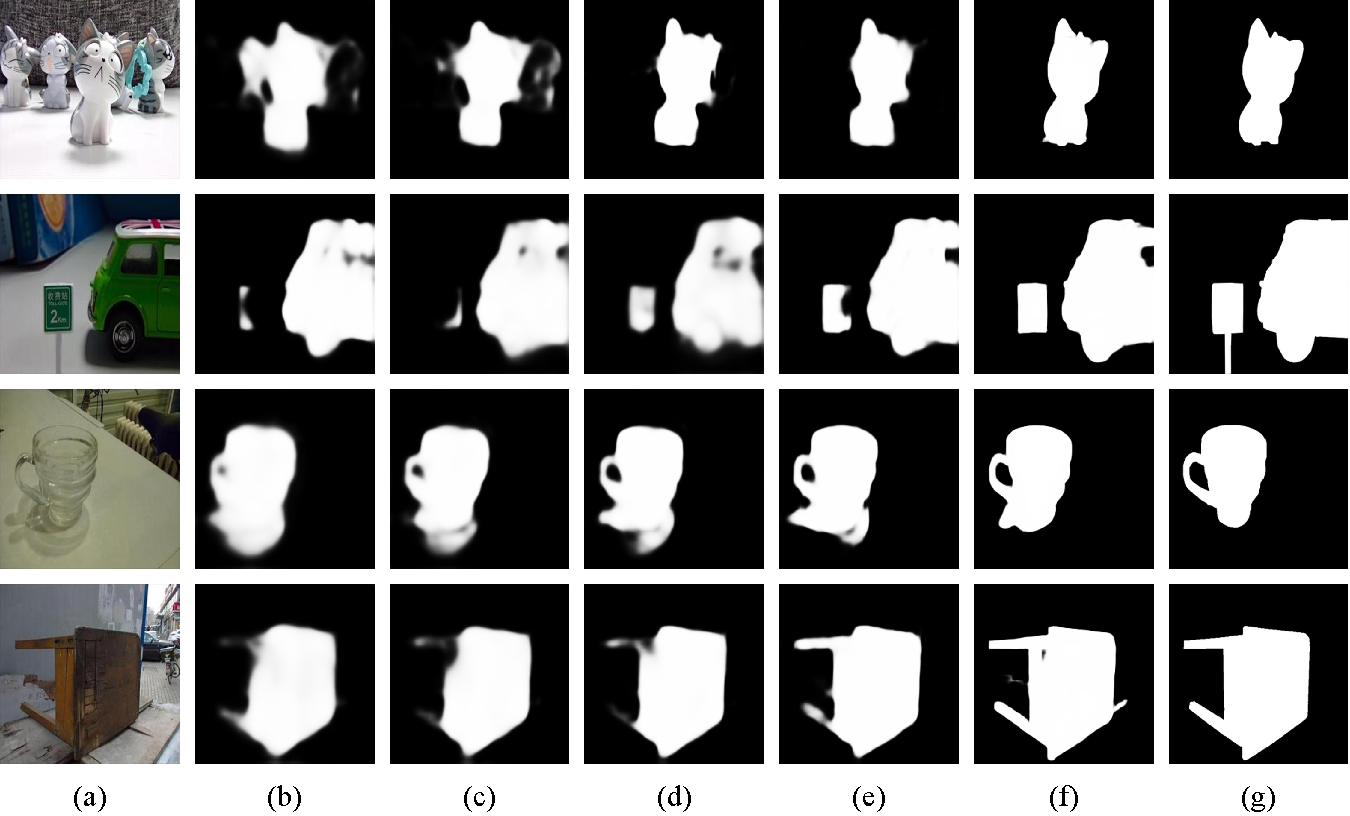
\includegraphics[width=0.99\linewidth]{figures/chapter3/self-comparsion-Use} 
	\centering
	\bicaption{
		消融研究的可视化比较
	}{
		Visual comparisons of ablation studies
	}
	\label{figure:self_comp}
\end{figure}



\begin{table}[t]
	\bicaption{在 DUTLF-FS 数据集上每个组件的消融分析}
	{Ablation analyses of each component on the DUTLF-FS dataset}
	\centering
	\label{table:abl_total}
	\label{chpt3:table:abl_total}
	%	\resizebox{0.82\linewidth}{!}{
		\begin{tabular}{cllcccc}
			\toprule[2pt]  %添加表格头部粗线
			%%  \multicolumn{1}{c}{ \multirow{2}*{Methods} }
			
			\multicolumn{1}{c}{ \multirow{2}*{No.}} 
			& \multicolumn{2}{c}{ \multirow{2}*{设置}}	
			& \multicolumn{4}{c}{DUTLF-FS} \\
				
			\cmidrule(r){4-7} 
			
			& & & $E_{\phi}^{max}\uparrow$ & $S_{\alpha }\uparrow $ & $F_{\beta}^{max}\uparrow$ & MAE$\downarrow$ \\
			
	
			\midrule
	
%			% 开始填写数据
			1 & \multicolumn{2}{l}{ Baseline }     & 0.947 & 0.894 & 0.901 & 0.048 \\ 
			
			%		 			\multicolumn{2}{l}{+Token} 	 & 0.959 & 0.918 & 0.926 & 0.037 \\ 
			
			\midrule
			
			2 & \multicolumn{1}{l}{ \multirow{2}*{+令牌通信模块}}	

			& \multicolumn{1}{c}{+令牌交互}  & 0.961 & 0.923 & 0.932 & 0.034 \\ 
			3 & & \multicolumn{1}{c}{++令牌移位} & 0.968 & 0.933 & 0.944 & 0.027 \\
			
			\midrule
			
			4 & \multicolumn{2}{l}{++~~~聚焦感知增强} 		
			& \textbf{0.972} & 0.941 & 0.952 & 0.022 \\
			
			5 & \multicolumn{2}{l}{+++特征融合模块} 		
			& \textbf{0.972} & \textbf{0.942} & \textbf{0.953} & \textbf{0.021} \\ 
			
			
			\bottomrule[2pt]
		\end{tabular}
		% }
\end{table}



%%%%%%%%%%%%%%%%%%%%%%%%%%%%%%%%%%%%%%%%%%%%%%%%%%%%%%%%%%%%%%
(2)定性比较:

为了更直观地观察,
图~\ref{figure:figure_comparison_1}~和
\ref{figure:figure_comparison_2}~
中可视化了所提出的方法和其他排名靠前的方法生成的一些代表性结果。可以看出,我们提出的方法的结果与真值图更加一致。 当面对这些具有挑战性的场景时,包括多个对象(第 4、5 行)和复杂场景(第 6、7 行),大多数 RGB 和 RGB-D 显著性检测方法无法准确检测显着对象。
相比之下,我们所提出的方法可以成功生成准确且稳健的显着图。 与这些基于 CNN 的 LFSOD 方法相比,所提出的方法获得了更一致的预测结果和更精细的细节。








%%%%%%%%%%%%%%%%%%%%%%%%%%%%%%%%%%%%%%%%%%%%%%%%%%%%%%%%%%%%%%
\BiSubsection{对比实验}{Comparative Experiment}

\textbf{不同模型组件的有效性。}
我们首先在表~\ref{table:abl_total}~中验证不同模型组件的有效性。
我们首先构建一个基线模型。 
具体来说,它使用共享权重编码器来提取全聚焦图和焦点堆栈特征,
然后在通道维度进行拼接,送入使用二维卷积网络构建的融合模块进行进一步的特征提取,
最后将融合后的特征送入显著性目标检测头并预测最终的显著性图。 




为了验证我们所提出的各个模块的有效性,
我们逐渐在基线网络中添加令牌交互模块,聚焦感知增强模块和特征融合模块
到我们的焦点感知网络中,在表~\ref{table:abl_total}~中分别以标号2,~4,~5表示。
如表~\ref{table:abl_total}~所示,这三个模型可以逐渐提高光场显著性目标检测性能,
最终大幅优于基线模型。 




此外,为了证明我们令牌交互模块中的令牌交互操作和令牌移位操作的有效性,
我们在表~\ref{table:abl_total}~中添加标号为2,3的网络,
分别表示我们只在基线模型上添加令牌交互操作,以及基于模型2,再添加令牌移位操作的网络。
从表中数据可以看出,与标号1的基线模型相比。
模型2和模型3在 DUTLF-FS 数据集上分别使 MAE 指标降低 29.2\% 和 43.8\%。 




%%%%%%%%%%%%%%%%%%%%%%%%%%%%%%%%%%%%%%%%%%%%%%%%%%%%%%%%%%%%%%%%%%%%%%%%%%%%%%%%%%
我们还在图~\ref{figure:self_comp}~中提供了每个消融研究相应的可视化结果,
其中(a)表示全聚焦图像,
(b)-(f) 分别代表基线模型、以及在基线模型基础上逐步添加
令牌交互模块,令牌移位模块、聚焦感知模块和特征融合模块的显著性目标预测图,
对应消融实验表~\ref{chpt3:table:abl_total}~中编号从1-5的不同设置的方法。
可以发现,预测的二进制掩码表示与真值图逐渐变得更加一致。 
显着对象的完整内容和精确的显着图边界,
证明我们的焦点感知Transformer模型可以有效过滤掉背景干扰并更多地关注显着对象。 






%---------------------------------------------------------------------> 消融实验: 焦点感知实验
%
\begin{table}[t]
	\bicaption{焦点相关令牌数量的影响, $M$表示焦点相关令牌的数量}
	{Impact of focal-related token numbers. $M $ indicates the number of focal-related tokens}
	\centering
	\label{table:abl_token_number}
	%	\resizebox{0.68\linewidth}{!}{
		\begin{tabular}{ccccc}
			\toprule[2pt]  %添加表格头部粗线
			
			% title
			\multirow{2}*{$M$} & \multicolumn{4}{c}{DUTLF-FS} \\ % & \multicolumn{3}{c}{HFUT} \\
			
			% next line
			\cmidrule(r){2-5} % \cmidrule(r){5-7} % \cmidrule(r){7-8} 
			
			% subtitle
			& $E_{\phi}^{max}\uparrow$ & $S_{\alpha }\uparrow $ & $F_{\beta}^{max}\uparrow$ & MAE$\downarrow$\\
			% & $S_{\alpha }\uparrow $ & $F_{\beta}^{max}\uparrow$ & MAE$\downarrow$ \\
			
			\midrule
			
			% 开始填写数据
			%% 8 & 0.969 & 0.934 & 0.944 & 0.026 \\ 
			
			8 &  0.967 & 0.936 & 0.946 & 0.025 \\ 
			16 & 0.970 & 0.937 & 0.948 & 0.024 \\
			32 & \textbf{0.972} & \textbf{0.941} & \textbf{0.952} & \textbf{0.022} \\ 
			
			\bottomrule[2pt]
		\end{tabular}
		%	}
	
\end{table}



 

\textbf{焦点相关标记的数量。} 
在表~\ref{table:abl_token_number}~中,我们用焦点相关标记的数量从 8 个增加到 32 个来测试我们的方法。与较少的焦点相关标记 (M = 8, 16) 相比,更多的焦点相关标记 (M = 32) 可以获得更好的结果 。 除非另有说明,我们的实验均使用 32 个与焦点相关的标记进行。 


% 
%---------------------------------------------------------------------> 消融实验: 焦点感知实验
%
\begin{table}[t]
	\bicaption{焦点感知增强策略中使用的不同K数的比较}
	{Comparison of using different K numbers in focal perception enhancement strategy}
	\centering
	\label{table:abl_fp}
	%	\resizebox{0.68\linewidth}{!}{
		\begin{tabular}{ccccc}
			\toprule[2pt]  %添加表格头部粗线
			
			% title
			\multirow{2}*{K} & \multicolumn{4}{c}{DUTLF-FS} \\ % & \multicolumn{3}{c}{HFUT} \\
			
			% next line
			\cmidrule(r){2-5} % \cmidrule(r){5-7} % \cmidrule(r){7-8} 
			
			% subtitle
			& $E_{\phi}^{max}\uparrow$ & $S_{\alpha }\uparrow $ & $F_{\beta}^{max}\uparrow$ & MAE$\downarrow$\\
			% & $S_{\alpha }\uparrow $ & $F_{\beta}^{max}\uparrow$ & MAE$\downarrow$ \\
			
			\midrule
			
			% 开始填写数据
			1 & 0.969 & 0.934 & 0.944 & 0.026 \\ 
			3 & 0.969 & 0.937 & 0.947 & 0.024 \\ 
			5 & \textbf{0.972} & \textbf{0.941} & \textbf{0.952} & \textbf{0.022} \\ 
			7 & 0.971 & 0.940 & 0.951 & \textbf{0.022} \\ 
			9 & 0.971 & 0.938 & 0.951 & 0.023 \\ 
			
			\bottomrule[2pt]
		\end{tabular}
		%	}
\end{table}

\textbf{焦点感知增强中的 $K$ 值。 }
我们设置了多个比较实验来选择最佳 $k$ 数,具体数据见表~\ref{table:abl_fp}。
当我们将 $K$ 从 1 增加到 5 时,性能逐渐提高。 当 $K > 5$ 时,我们观察到模型性能饱和并变得次优。 我们认为较大的 $K$ 值会引入更多不显着的背景效应。 考虑到性能和计算成本之间的权衡,我们选择配置 $K = 5$ 作为最终配置。



%%%%%%%%%%%%%%%%%%%%%%%%%%%%%%%%%%%%%%%%%%%%%%%
\textbf{焦点感知增强方法设置。}
为了验证不同焦点感知增强设置的有效性,我们在随机、卷积和基于 SSIM 的选择方法之间进行了比较实验。 所有实验将 $K$ 数设置为 5。表~\ref{table:abl_methods}~表明我们使用基于卷积方式进行感知增强的方法已经达到了与其他光场显著性检测方法相当的性能,证明了我们提出的方法的优越性。


\begin{table}[t]
	\bicaption{焦点感知增强模块中不同方法的消融结果}
	{Ablation results of different methods for focal perception enhancement module}
	\centering
	\label{table:abl_methods}
	%	\resizebox{0.45\linewidth}{!}{
		\begin{tabular}{ccccc}
			\toprule[2pt]  %添加表格头部粗线
			
			% title
			\multirow{2}*{Settings} & \multicolumn{4}{c}{DUTLF-FS} \\  % & \multicolumn{3}{c}{HFUT} \\
			
			% next line
			\cmidrule(r){2-5} % \cmidrule(r){5-7} % \cmidrule(r){7-8} 
			
			% subtitle
			& $E_{\phi}^{max}\uparrow$ & $S_{\alpha }\uparrow $ & $F_{\beta}^{max}\uparrow$ & MAE$\downarrow$ \\
			% & $S_{\alpha }\uparrow $ & $F_{\beta}^{max}\uparrow$ & MAE$\downarrow$ \\
			
			\midrule
			
			% 开始填写数据
			Random      & 0.962 & 0.924 & 0.932 & 0.033 \\ 
			Conv        & 0.967 & 0.931 & 0.942 & 0.027 \\ 
			SSIM        & \textbf{0.972} & \textbf{0.941} & \textbf{0.952} & \textbf{0.022} \\ 
			%% Log(SSIM)   & \textbf{0.972} & 0.940 & 0.950 & 0.023 \\ 
			
			\bottomrule[2pt]
		\end{tabular}
		%}
\end{table}





%%%%%%%%%%%%%%%%%%%%%%%%%%%%%%%%%%%%%%%%%%%%%%%
\BiSection{本章小结}{The Chapter’s Conclusion}

在本文中,我们提出了一种用于精确光场显着物体检测的焦点感知Transformer(FPT)。 我们引入与焦点相关的令牌来收集图像特定的特征,并提出令牌通信模块(TCM)来传播信息并促进空间上下文建模。 为了增强焦点堆栈的空间特征表示,我们提出了一种焦点感知增强(FPE)策略来帮助抑制噪声背景信息。 实验结果表明,我们提出的方法可以在大多数光场显著性分割数据集上实现最先进的性能。
\BiChapter{基于视角增强的光场显著性目标检测}{TODO}
\label{chap:part4}
%
%
%
%
第三章从焦点感知的角度出发,设计了一种切片级探索多视角场景聚焦信息的显著性目标检测算法。
该方法注重对多视角三维场景的感知,以及不同视角对显著性预测的贡献程度,
实现了光场信息的深度挖掘以及多视角信息的高效探索。
%
%
本章从视角强化的角度出发,基于注意力机制引入视角增强模块,并通过前背景的补偿模块优化网络的训练,
实现了光场信息的充分挖掘。
%
%
%
%
\BiSection{研究动机}{TODO}
%
%
%
%
光场技术可以完整地记录场景的几何信息。在其中,焦点堆栈数据是光场数据的关键表达形式之一。现有研究表明,光场数据在显著性目标检测方面具有优势。
随着基于Transformer架构的模型在各种视觉任务上取得超越性的性能,基于Transformer架构的光场显著性检测网络也逐渐出现\cite{wang2023tenet,liu2023lftransnet}。
然而,直接应用Transformer架构到光场显著性检测任务中,
并不能充分发挥Transformer架构对于长距离建模的能力,
不能得到理想的光场显著性目标检测效果。
还要设计合适的网络结构,加强模型对光场中隐含空间场景的感知,
来使得模型对光场显著性检测有一个鲁棒性的结果。
%
%
%
%
\par
\begin{figure}[!ht]
	\centering
	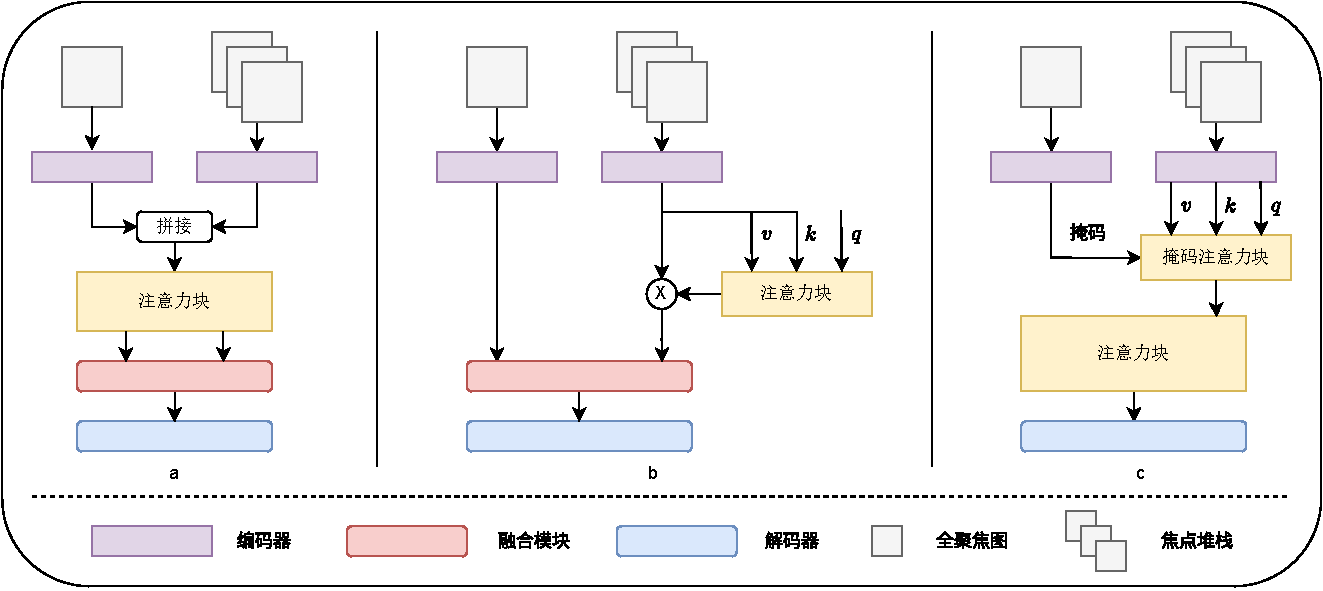
\includegraphics[width=0.95\linewidth]{figures/chapter4/task2_ins.drawio}
	\bicaption{光场模型范例}{TODO}  
	\label{cpt4_fig1:task2_ins}
\end{figure}
%
%
%
%
王等人~\cite{wang2023tenet}通过拼接焦点堆栈和全聚焦图特征,
一并送入Transformer编码器来,建立光场整体结构的感知模型。
如图~\ref{cpt4_fig1:task2_ins}~(a)~所示,
但是这种方式弱化了全聚焦图片特征和散焦图片特征之间的模态差异,两个模态之间的融合依然依赖后续的融合模块。
刘等人~\cite{liu2023lftransnet}只在焦点堆栈支路使用了Transformer结构。该方法聚合多尺度的焦点堆栈特征构造注意力矩阵,用一个可学习的权重来作为查询矩阵。通过注意力运算来汇总不同切片对显著性检测的贡献。如图~\ref{cpt4_fig1:task2_ins}~(b)~所示。
%
%
但是,这些方法没有充分考虑两个模态之间的差异,融合方式有限,起到的特征强化效果也有限。


针对上述问题,本章提出来一种基于视角增强的光场显著性目标检测方法。
此方法致力于从焦点堆栈和全聚焦图的差异入手,结合Transformer强大的注意力机制,提出了合成增强视角的注意力方法。


~

随着



然而,采集光场数据需要多组摄像头或相机矩阵,造成了高昂的成本。为了实现理想的光场显著性目标检测能力,除了设计合适的网络模型外,还需要大量高质量的光场数据。由于光场数据获取成本高,目前的方法通常采用数据增强手段来增加训练数据。传统的数据增强方法包括旋转、平移、裁剪和缩放等操作,但这些方式的变化有限,效果也不够显著。对于不同类型的光场数据,需要不同的增强方法,选择不当的方法可能会引入噪声,导致训练不稳定,降低模型性能。因此,如何稳定生成高质量的光场数据以实现数据增强的目标是当前需要解决的问题。



针对上述问题。  
  
为验证本方法的有效性,本章在 DUT-LFSD, LFSD 以及 HFUT-LFSD
数据集上进行了实验,同样获得了超越传统数据增强手段的性能,为光场数据的应用奠
定了基础。为了进一步验证本方法的有效性,本章将提出的数据增强方法应用在当前最
好的光场显著性检测方法上,实验结果表明,本章的数据增强方法能够提升其它方法的
检测性能。



% task2_ins.drawio


\BiSection{方法介绍}{TODO}





%
%
%
%
\BiSubsection{视角增强模块}{TODO}

\BiSubsection{感知学习策略}{TODO}

\BiSubsection{训练过程}{TODO}


%\\
%\\
%\\
%\\
\BiSection{实验结果与分析}{TODO}

\BiSubsection{实验设置}{TODO}

\BiSubsection{消融实验}{TODO}

\BiSubsection{对比实验}{TODO}


%\\
%\\
%\\
%\\
\BiSection{本章总结}{TODO}




\BiChapter{注释(需要删除)}{uuu}
%\caption{u}



%
%
%最近,光场显著性物体检测(LFSOD)因在复杂场景中利用丰富的光场线索取得显著改进而引起了越来越多的关注。虽然许多工作在这一领域取得了显著进展,但对其焦点特性的更深入洞察应该被开发。在这项工作中,我们提出了焦点感知变换器(FPT),可以高效地编码焦点堆栈内和全部焦点图像中的上下文。具体而言,我们引入了与焦点相关的令牌来总结图像特定特征,并且提出了令牌通信模块(TCM)来传达信息并促进空间上下文建模。通过精确编码的与焦点相关的令牌之间的信息交换,可以丰富每幅图像的特征并与其他图像相关联。我们还提出了焦点感知增强(FPE)策略,以帮助抑制嘈杂的背景信息。对四个广泛使用的基准数据集进行的大量实验证明,所提出的模型优于当前最先进的方法。我们的代码将公开提供。




% 
% 
% 
% 
% <<<<<<< HEAD
% 其中$m$索引注意力头,$k$索引采样键,
% $K$是采样键的总数($K \ll HW$),
% $\bigtriangleup p_{mqk} $和$A_{mqk}$分别表示
% 第$m^{th}$个注意力头中第$k^{th}$个采样点的采样偏移量和注意力权重。
% 标量注意力权重$A_{mqk}$位于$\left [ 0,~1 \right ] $范围内,
% 通过$ {\textstyle \sum_{k=1}^{K}} A_{mqk}=1$进行归一化。
% $\bigtriangleup p_{mqk} \in \mathbb{R}^{2}$
% 是范围不受约束的二维实数。
% 由于$p_{q} + \bigtriangleup p_{mqk}$是分数,如等人所述,
% $x\left ( p_{q} + \bigtriangleup p_{mqk} \right ) $在计算时应用双线性插值。
% $\bigtriangleup p_{mqk}   $和$A_{mqk}$都是通过查询特征$z_{q}$上的线性投影获得的。
% 在具体实现中,查询特征$z_{q}$被馈送到$3MK$通道的线性投影算子,
% 其中前$2MK$通道对采样偏移量$\bigtriangleup p_{mqk}$进行编码,
% 其余$MK$通道通过被馈送到$softmax$算子以获得注意力权重$A_{mqk}$。






% 可变形注意力模块旨在将卷积特征图作为关键元素进行处理。

% 设 为查询元素的数量,当较小时,可变形注意力模块的复杂度为。
% 当应用于DETR编码器时,其中,复杂度变为,
% 起复杂度与空间大小呈线性关系。
% 当它作为DETR解码器中的交叉注意力模块应用时,
% 其中,是对象查询的数量,复杂度变为,
% 这与空间大小无关。


% 多尺度可变形注意力模型。
% 大多数现代目标检测框架都受益于多尺度特征图。
% 我们提出的可变形注意力模块可以自然地扩展到多尺度特征图。
% 令为输入多尺度特征图,
% 其中。
% 令为每个查询元素的参考点的归一化坐标,
% 然后应用多尺度可变形注意力采样点。
% 分别表示第几个特征层和第几个注意力头中第几个采样点的采样偏移和注意力权重。
% 标量注意力权重通过进行归一化。

% 这里,为了尺度公式的清晰性,我们使用归一化坐标,
% 其中归一化坐标分别表示图像的左上角和右下角。
% 方程中的函数将归一化坐标重新放缩到第几层的输入特征图。


% 多尺度可变形注意力与之前的单尺度版本非常相似,只是它从多尺度特征图中采样点,
% 而不是从单尺度特征图中采样k个点。
% 当且固定为单位矩阵时,所提出的注意力模块将退化为可变形卷积。
% 可变形卷积是针对单尺度输入而设计的,每个注意力头仅关注一个采样点。
% 然而,我们的多尺度可变形注意力会关注来自多尺度输入的多个采样点。
% 所提出的(多尺度)可变形注意模块也可以被视为
% Transformer 注意的有效变体,其中通过可变形采样位置引入预过滤机制。
% 当采样点遍历所有可能得位置时,所提出的注意力模块相当于Transformer注意力。


% 可变形Transformer 编码器。

% 我们将网络中处理特征图的Transformer注意模块替换为所提出的多尺度可变形注意模块。
% 编码器的输入和输出都是具有相同分辨率的多尺度特征图。

% 在编码器中,我们从骨干网络中提取多尺度特征图,通过卷积,
% 其中的分辨率比输入图像低。
% 最低分辨率特征图是通过最后阶段的步长卷积获得的。

% 所有多尺度特征图均为个通道,
% 像FPN网络结构中,没有使用自上而下的结构,因为我们提出的多尺度可变形注意力本身可以在多尺度特征图之间交换信息。




%%
%%
%\begin{table*}[]
%	%
%	%---------------------------------------------------------------------> 大表 
%	%
%	%	\caption{Quantitative comparison of our proposed FPT with other 20 SOTA SOD methods on three benchmark datasets. 
%		%		$ \uparrow \& \downarrow $ denote larger and smaller is better.
%		%		%
%		%		% denote the best and the second-best results,
%		%		%
%		%		The best three results are shown in 
%		%		\textbf{boldface}, \textcolor{red}{red} and \textcolor{blue}{blue} fonts respectively. 
%		%		% '-' indicates the code or outcome is not available.
%		%	}
%	\bicaption{
%		在 3 个公开数据集上的定量比较
%	}{Quantitative comparisons on three light field datasets}
%	%	\renewcommand{\arraystretch}{1.5}
%	
%	\centering
%	\label{table:comp_with_sota_3_1}
%	%	\label{table:comp-with-sota}
%	\resizebox{\textwidth}{!}{
%		\begin{tabular}{rcccccccccccc}
%			\toprule  %添加表格头部粗线
%			
%			% title
%			%			\multirow{2}*{Type} & 
%			\multicolumn{1}{c}{ \multirow{2}*{方法} } & 
%			\multicolumn{4}{c}{DUTLF-FS \cite{zhang2019memory} } &
%			\multicolumn{4}{c}{HFUT \cite{zhang2017saliency} } &
%			\multicolumn{4}{c}{LFSD \cite{li2014saliency} } \\
%			
%			% next line
%			\cmidrule(r){2-5} \cmidrule(r){6-9} \cmidrule(r){10-13}
%			
%			%			 subtitle
%			& $E_{\phi}^{max}\uparrow$ & $S_{\alpha }\uparrow$ & $F_{\beta}^{max}\uparrow$ & MAE$\downarrow$ 
%			& $E_{\phi}^{max}\uparrow$ & $S_{\alpha }\uparrow$ & $F_{\beta}^{max}\uparrow$ & MAE$\downarrow$  
%			& $E_{\phi}^{max}\uparrow$ & $S_{\alpha }\uparrow$ & $F_{\beta}^{max}\uparrow$ & MAE$\downarrow$ \\
%			
%			%			& E & S & F & MAE 
%			%			& E & S & F & MAE 
%			%			& E & S & F & MAE \\
%			
%			
%			% line line
%			\midrule
%			
%			%			\multirow{8}*{\textit{Light field}}
%			
%			% 开始填数据
%			
%			Ours	 
%			&  {\textbf{.973}} & \textbf{ {.946}} 	& \textbf{ {.954}} & \textbf{ {.020}} 
%			& \textbf{ {.871}} &	\textbf{ {.828}} 			&\textbf{	 {.784}} & {\textcolor{red}{.064}} 
%			& \textbf{ {.919}} &	\textcolor{blue}{.860} 			&	\textbf{ {.873}} &	\textbf{ {.064}} 
%			\\
%			
%			DLGLRG \cite{liu2021light} 
%			& {\textcolor{red}{.958}} & {\textcolor{red}{.928}} 			& {\textcolor{red}{.934}} & {\textcolor{red}{.029}} 
%			&	.839 &	.766 &	.698 &	.070 
%			&	{\textcolor{red}{.906}} &	\textbf{ {.866}} 			&	{\textcolor{red}{.870}} &	\textcolor{blue}{.069} 
%			\\
%			
%			ERNet \cite{piao2020exploit}
%			& .947 & .899 & .908 & .039 
%			&	.841 &	.778 &	.722 &	.082 
%			&	.888 &	.834 &	.850 &	.082 
%			\\
%			
%			PANet \cite{piao2021panet} 
%			& .939 & .908 & .903 & .038 
%			& .845 & .795 & .738 & .074 
%			& .892 & .849 & .849 & .076
%			\\
%			
%			LFNet	 \cite{zhang2020lfnet} 
%			& .929 & .878 & .890 & .053
%			&	.846 &	.782 &	.718 &	.073 
%			&	.885 &	.820 &	.824 &	.092 \\
%			
%			MAC	 \cite{zhang2020light} 
%			& .863	& .804	& .792	& .102	
%			&   .797 & .731 & .667 & .107 
%			& .832 & .782 & .776 & .127 \\
%			
%			MoLF	 \cite{zhang2019memory} 
%			& .938 & .887 & .902 & .051 
%			&	.852 &	.789 &	.729 &	.075 
%			&	.888 &	.830 &	.834 &	.089 \\
%			
%			DLSD	\cite{piao2019deep}
%			& .891	& .841	& .801	& .076	
%			&   .783 & .741 & .615 & .098 
%			& .806 & .737 & .715 & .147 \\
%			
%			\midrule % end lfsod
%			
%			% start rgb-d
%			%			\multirow{6}*{\textit{RGB-D}}
%			
%			DCF \cite{ji2021calibrated} 
%			& \textcolor{blue}{.954} & \textcolor{blue}{.921} & \textcolor{blue}{.927} & \textcolor{blue}{.031} 
%			& \textcolor{blue}{.856} & {\textcolor{red}{.812}} & {\textcolor{red}{.768}} & \textcolor{blue}{.065} 
%			& .881 & .809 & .821 & .096 \\
%			
%			CIR-Net \cite{cong2022cir}
%			& .950 & .916 & .921 & .038 
%			& {\textcolor{red}{.862}} & .800  			& .742 & \textbf{ {.062}} 
%			& .874 & .820 & .816 & .098 \\ 
%			
%			VST-$rgbd$  \cite{liu2021visual} 
%			& .952 & .920 & .921 & .036 
%			& .843 & .807 & .754 & .086 
%			& .851 & .792 & .786 & .110 
%			\\
%			
%			%			& -  & 2022  & \\
%			%			& -  & 2022  & \\
%			
%			BBS-Net     \cite{fan2020bbs} 
%			& .900 & .865 & .852 & .066 
%			& .801 & .751 & .676 & .073 
%			& \textcolor{blue}{.901} & {\textcolor{red}{.864}} & .858 & .072 \\ 
%			
%			SSF     \cite{zhang2020select} 
%			& .922 & .879 & .887 & .050 
%			& .816 & .725 & .647 & .090 
%			& \textcolor{blue}{.901} & .859 & \textcolor{blue}{.868} & {\textcolor{red}{.067}} \\ 
%			
%			S2MA    \cite{liu2020learning} 
%			& .839 & .787 & .754 & 	.102 
%			& .777 & .729 & .650 & .112 
%			& .873 & .837 &	.835 & .094 \\
%			
%			
%			\midrule % end rgb-d
%			%			\multirow{7}*{\textit{RGB}}
%			
%			VST-$rgb$ \cite{liu2021visual} 
%			& .939 & .910 & .911 & .047
%			& .831 & \textcolor{blue}{.808} & \textcolor{blue}{.763} & .093 
%			& .865 & .797 & .817 & .123 
%			\\ 
%			
%			PFSNet \cite{ma2021pyramidal}
%			& .912 & .883 & .879 & .057 
%			& .835 & .800 & .752 & .088 
%			& .805 & .749 & .727 & .145 
%			\\ 
%			
%			
%			ITSD \cite{zhou2020interactive} 
%			& .930 & .899 & .899 & .052 
%			& .839 & .805 & .759 & .089 
%			& .879 & .847 & .840 & .088 
%			\\ 
%			
%			
%			
%			LDF \cite{wei2020label} 
%			& .898 & .873 & .861 & .061 
%			& .804 & .780 & .708 & .093 
%			& .843 & .821 & .803 & .096 
%			\\ 
%			
%			
%			MINet \cite{pang2020multi} 
%			& .916 & .890 & .882 & .050 
%			& .816 & .792 & .720 & .086 
%			& .861 & .834 & .828 & .091 
%			\\ 
%			
%			F$^{3}$Net  \cite{wei2020f3net}
%			& .900 & .888 & .882 & .057 
%			& .815 & .777 & .718 & .095 
%			& .824 & .806 & .797 & .106 
%			\\ 
%			
%			
%			EGNet   \cite{zhao2019egnet}
%			& .914 & .886 & .870 & .053 
%			& .794 & .772 & .672 & .094 
%			& .776 & .784 & .762 & .118 
%			\\ 
%			
%			CPD  \cite{wu2019cascaded}
%			& .867 & .911 & .866 & .058 
%			& .772 & .82  & .701 & .086 
%			& .759 & .82  & .759 & .126 \\
%			
%			PoolNet \cite{liu2019simple}
%			& .889 & .919 & .868 & .051 
%			& .776 & .802 & .683 & .092 
%			& .789 & .8   & .769 & .118 \\
%			
%			PiCANet \cite{liu2018picanet}
%			& .829 & .892 & .821 & .083 
%			& .726 & .781 & .618 & .115 
%			& .729 & .78  & .671 & .158 \\
%			
%			PAGRN \cite{wang2018detect}
%			& .822 & .878 & .828 & .084 
%			& .717 & .773 & .635 & .114 
%			& .727 & .805 & .725 & .147 \\
%			
%			C2S   \cite{li2018contour}
%			& .844 & .874 & .791 & .084 
%			& .763 & .786 & .65  & .111 
%			& .806 & .82  & .749 & .113 \\
%			
%			R3Net  \cite{deng2018r3net}
%			& .833 & .819 & .783 & .113 
%			& .727 & .728 & .625 & .151 
%			& .789 & .838 & .781 & .128 \\
%			
%			Amulet \cite{zhang2017amulet}
%			& .847 & .882 & .805 & .030 
%			& .767 & .76  & .636 & .110  
%			& .773 & .821 & .757 & .135 \\
%			
%			
%			\bottomrule % end
%		\end{tabular}
%	}
%\end{table*}
%%
%%
%%\\
%%\\


































%
%%
%%
%%\par
%\begin{figure}[!ht]
%	\centering
%	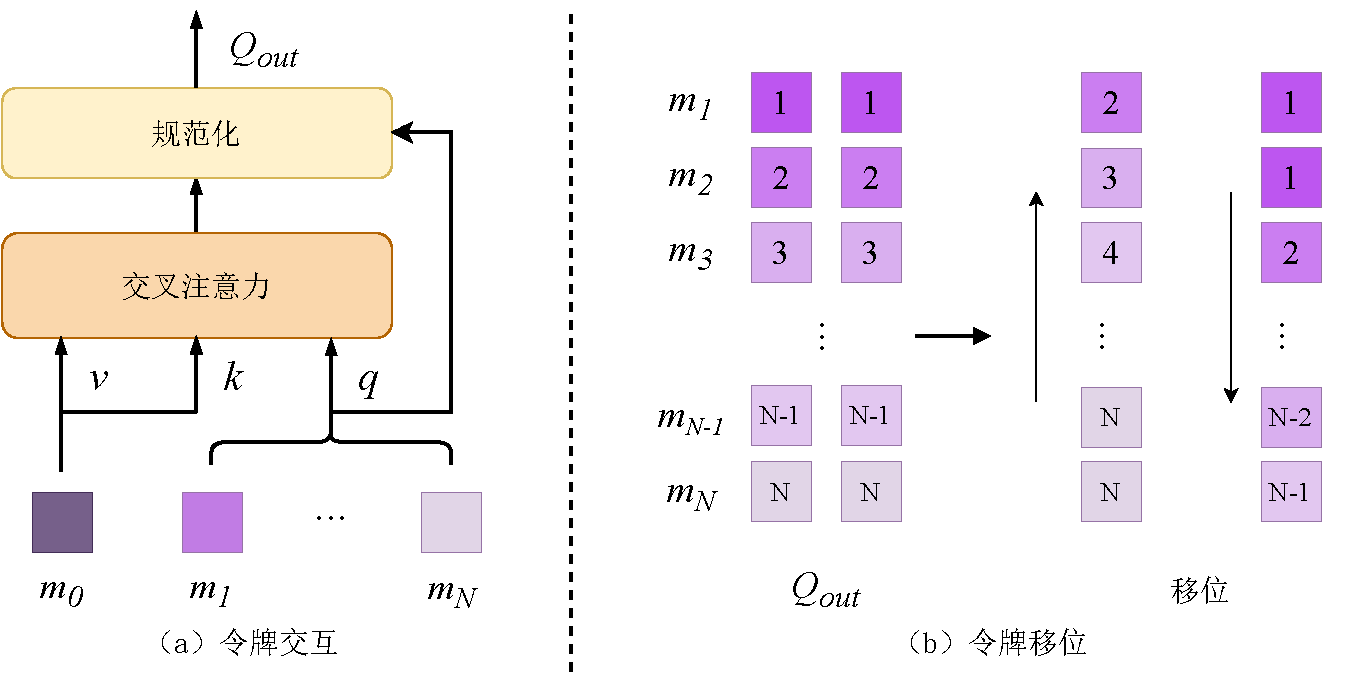
\includegraphics[width=0.95\linewidth]{figures/chapter3/token-interaction.drawio}
%	\bicaption{
%		令牌通信模块 (TCM) 的图示。
%		(a) 令牌交互(TI)。 
%		(b) 令牌移位(TS)。 
%	}{
%		An illustration of the Token Communication Module (TCM). 
%		(a) Token Interaction (TI). 
%		(b) Token Shift (TS).
%	}  
%	\label{cpt3_fig1:token_interaction}
%\end{figure}
%%
%%
















%
%
%%
%%---------------------------------------------------------------------> fig: 创新图
%\begin{figure}[!ht]
%	\centering
%	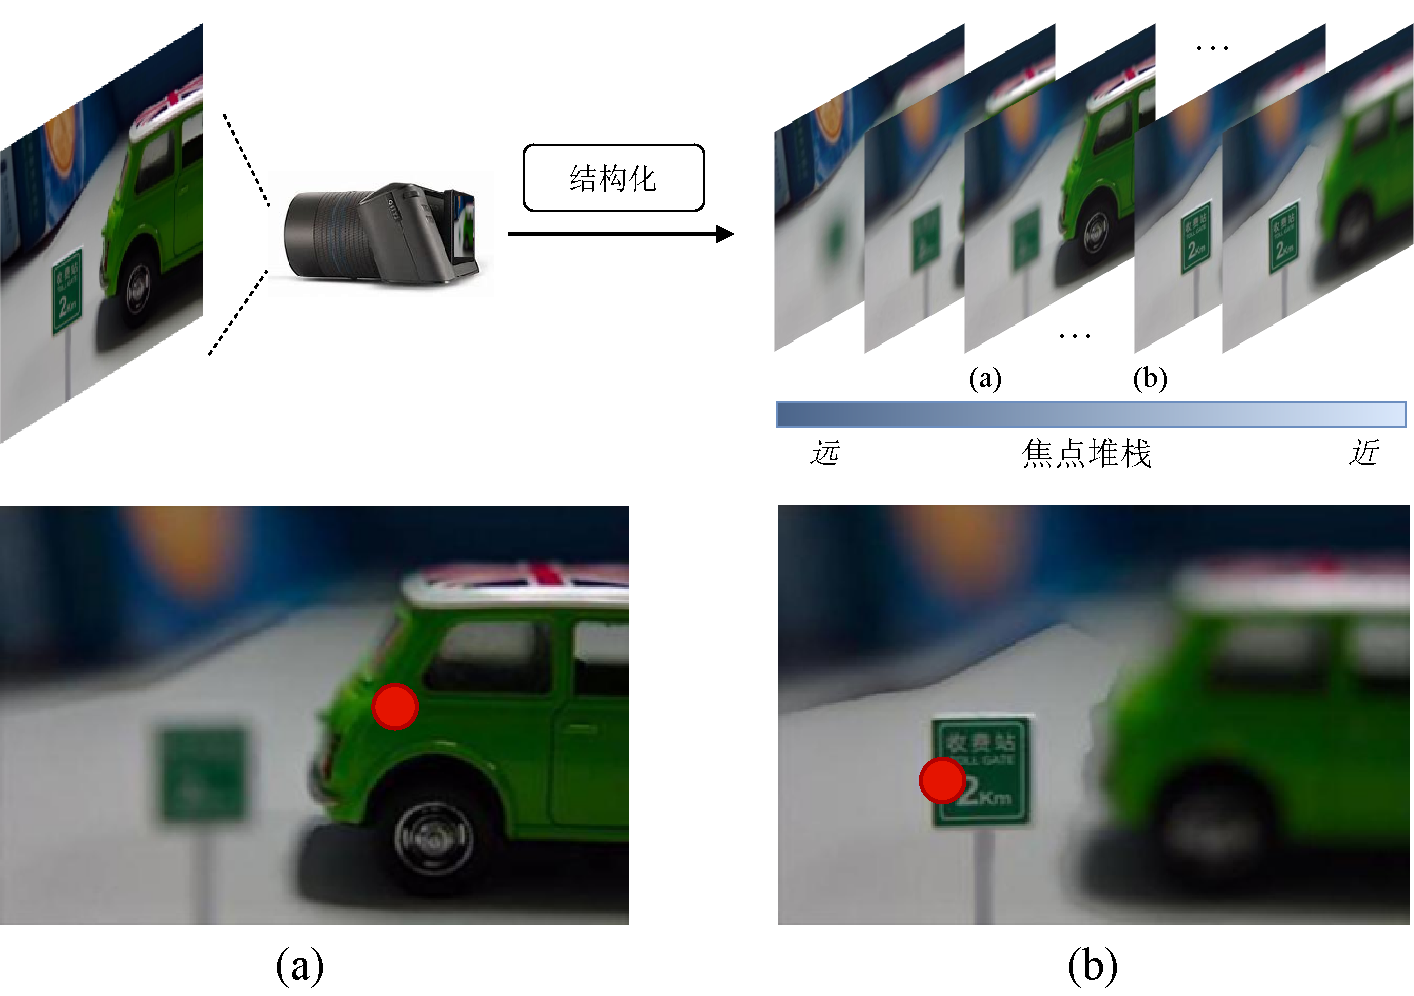
\includegraphics[width=0.85\linewidth]{figures/chapter3/cpt3_idea.pdf}
%	\bicaption{
%		光场焦点堆栈的成像过程和不同切片的成像效果。
%		\textcolor{red}{$\bullet$} 表示清晰的部分。
%	}
%	{ 
%		The imaging process of the light field focus stack and the imaging effects of different slices.
%		\textcolor{red}{$\bullet$} indicates the clear parts.  
%	}
%	\label{figure:cpt3:idea}
%\end{figure}
%%
%%


















%
%%------------------------------ figure: comparison
%\begin{figure}[!ht]
%	\centering
%	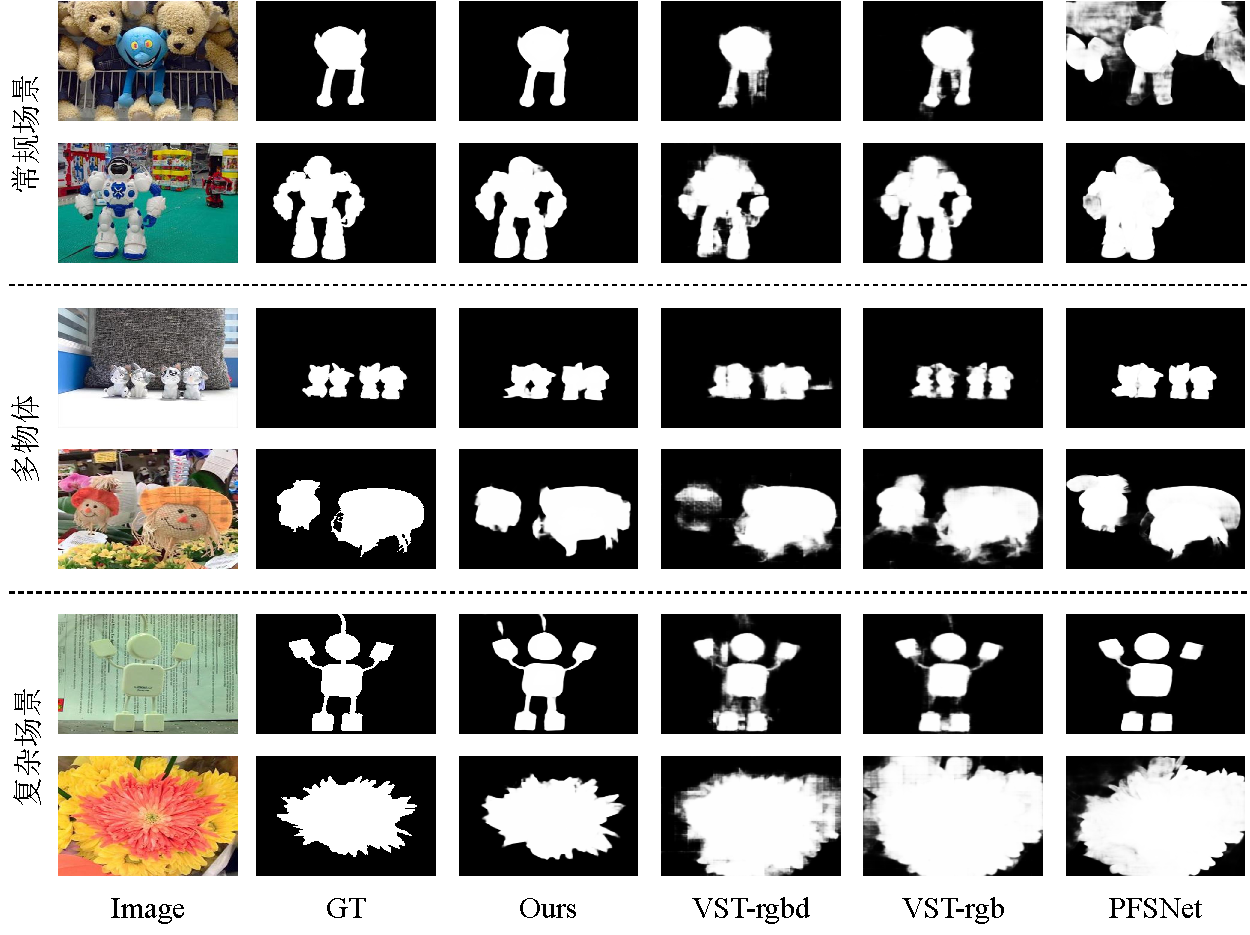
\includegraphics[width=\linewidth]{figures/chapter3/compare_3}
%	%	\caption{
%		%		Qualitative comparisons of state-of-the-art methods in some challenging scenes, including multiple objects and complex scenes.
%		%	}
%	\bicaption{
%		在一些具有挑战性的场景(包括多物体和复杂场景)中对最先进的方法进行定性比较。
%	}{
%		Qualitative comparisons of state-of-the-art methods in some challenging scenes, including multiple objects and complex scenes.
%	}
%	\label{chpt4:fig:comparison_3}
%	\vspace{-0.2cm}
%\end{figure}
%% 
%%
%










%
%\begin{figure}[!ht] 
%	% \centering
%	%	\begin{center}
%		%	\includegraphics[width=0.95\linewidth]{figures/overview.pdf} 		
%		%	\end{center}
%	
%	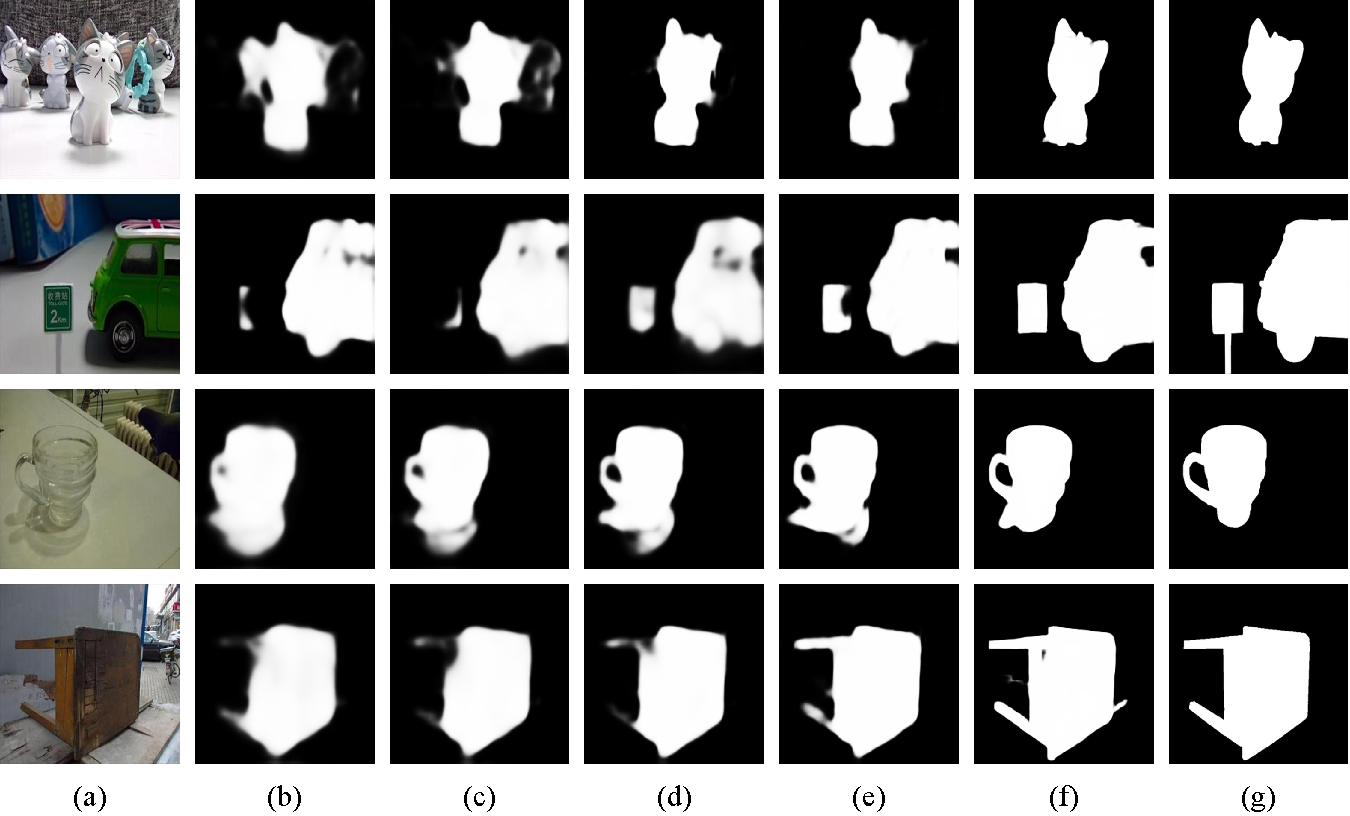
\includegraphics[width=0.99\linewidth]{figures/chapter3/self-comparsion-Use} 
%	\centering
%	
%	
%	%	\caption{   	Visual comparisons of ablation studies.      (a) All-focal images.      
%		%		(b)-(f) Saliency maps of the ``Baseline'', ``+TCM (+TI)'', ``+TCM (++TS)'', ``++FPE'' and ``+++CCM'', respectively.
%		%		%			
%		%		%			(b) Saliency maps of baseline.
%		%		%			(c) Saliency maps w TCM (w/o TS).
%		%		%			(d) Saliency maps w TCM.
%		%		%			(e) Saliency maps w using FPE.
%		%		%			(f) Saliency maps w using CCM.
%		%		(g) Ground truth maps.
%		%	}  
%	%	
%	\bicaption{
%		消融研究的可视化比较。 
%		%	(a) 全聚焦图像,
%		%	(b)-(f) 分别为“基线模型”、
%		%	“+TCM (+TI)”、
%		%	“+TCM (++TS)”、
%		%	“++FPE”和
%		%	“+++CCM图”的显著性图。
%	}{
%		Visual comparisons of ablation studies.      
%		%	(a) All-focal images.      
%		%	(b)-(f) 
%		%	Saliency maps of the ``Baseline'', 
%		%	``+TCM (+TI)'', 
%		%	``+TCM (++TS)'', 
%		%	``++FPE'' and 
%		%	``+++CCM'', respectively.
%		%	(g) Ground truth maps.
%	}
%	\label{figure:self_comp}
%	
%	\vspace{-0.2cm}
%\end{figure}
%
%
















%
%%
%%\par
%\begin{figure}[!ht]
%	\centering
%	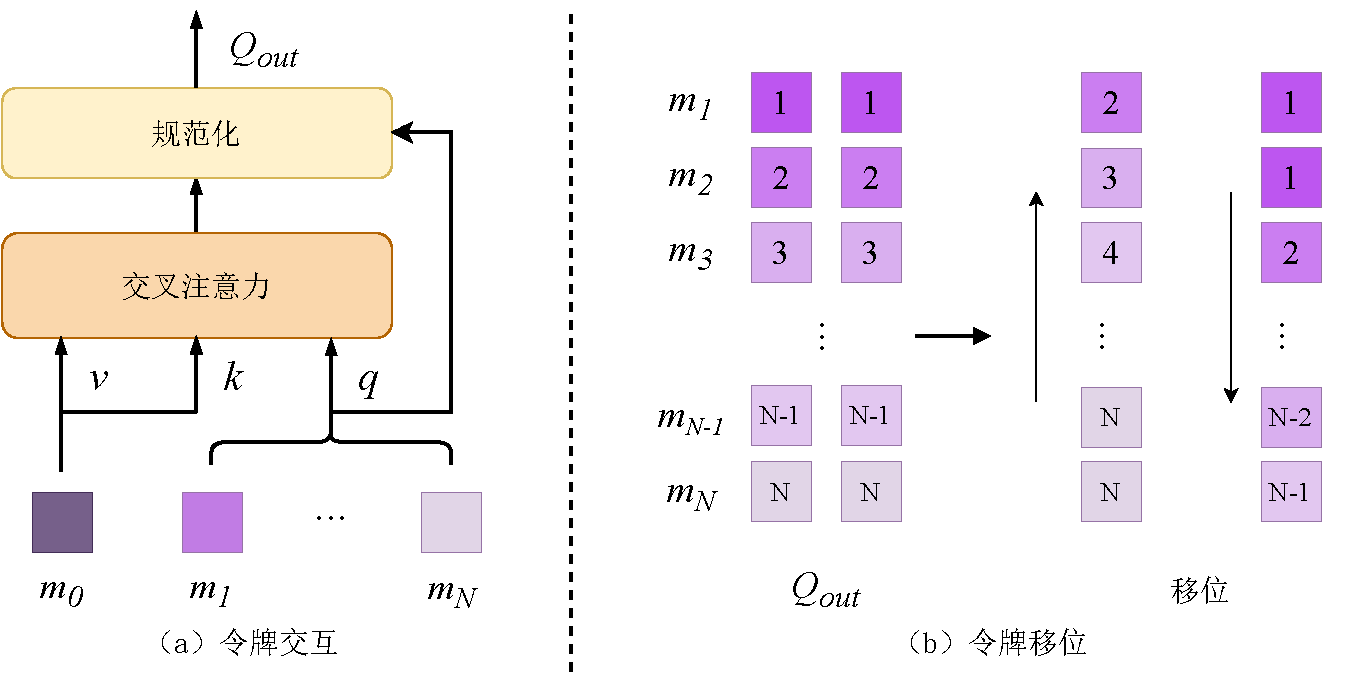
\includegraphics[width=0.95\linewidth]{figures/chapter3/token-interaction.drawio}
%	\bicaption{
%		令牌通信模块 (TCM) 的图示。
%		(a) 令牌交互(TI)。 
%		%		交叉注意力在全焦点和焦点堆栈的嵌入式令牌之间执行特征交互。 
%		(b) 令牌移位(TS)。 
%		%		仅将焦点堆栈流中与焦点相关的标记分成组(图中以2组为例),然后沿焦点深度轴以不同方向(左右)移位以交换切片级信息。
%	}{
%		An illustration of the Token Communication Module (TCM). 
%		(a) Token Interaction (TI). 
%		%	Cross-attention performs feature interactions between the all-focal and focal stack. 
%		(b) Token Shift (TS).
%		%	Only the focus-related tokens in the focus stack stream are split into groups (2 in the figure) and then circularly shifted along the focus-depth axis with different directions to exchange slice-level information.
%	}  
%	\label{cpt3_fig1:token_interaction}
%\end{figure}
%%
%%







%\begin{figure}[!ht]
%	\centering
%	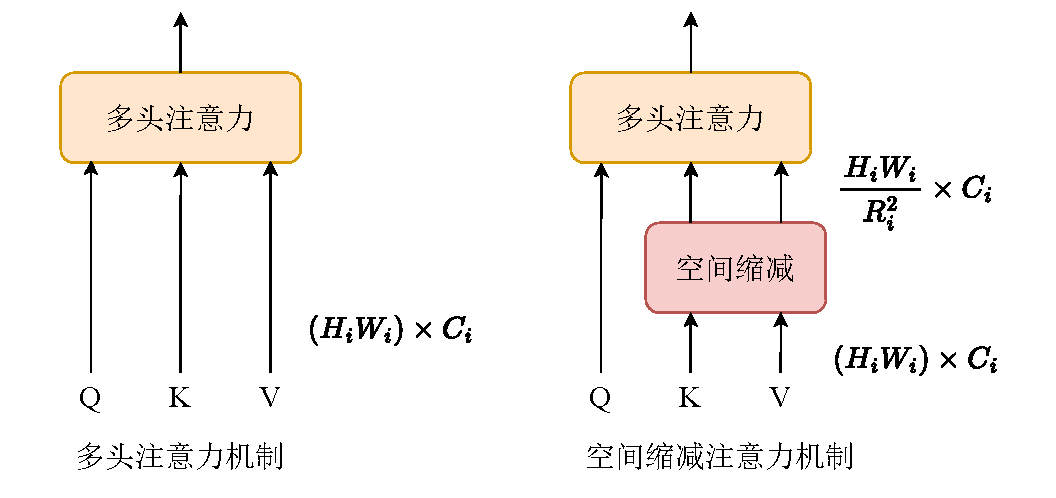
\includegraphics[width=0.95\linewidth]{figures/chapter3/sra}
%	\bicaption{
%		令牌通信模块 (TCM) 的图示。
%		(a) 令牌交互(TI)。 
%		%		交叉注意力在全焦点和焦点堆栈的嵌入式令牌之间执行特征交互。 
%		(b) 令牌移位(TS)。 
%		%		仅将焦点堆栈流中与焦点相关的标记分成组(图中以2组为例),然后沿焦点深度轴以不同方向(左右)移位以交换切片级信息。
%	}{
%		An illustration of the Token Communication Module (TCM). 
%		(a) Token Interaction (TI). 
%		%	Cross-attention performs feature interactions between the all-focal and focal stack. 
%		(b) Token Shift (TS).
%		%	Only the focus-related tokens in the focus stack stream are split into groups (2 in the figure) and then circularly shifted along the focus-depth axis with different directions to exchange slice-level information.
%	}  
%	\label{cpt3_fig1:sra}
%\end{figure}
%%
%%


%
%
%---------------------------------------------------------------------> fig: 创新图
%\begin{figure}[!ht]
%	\centering
%	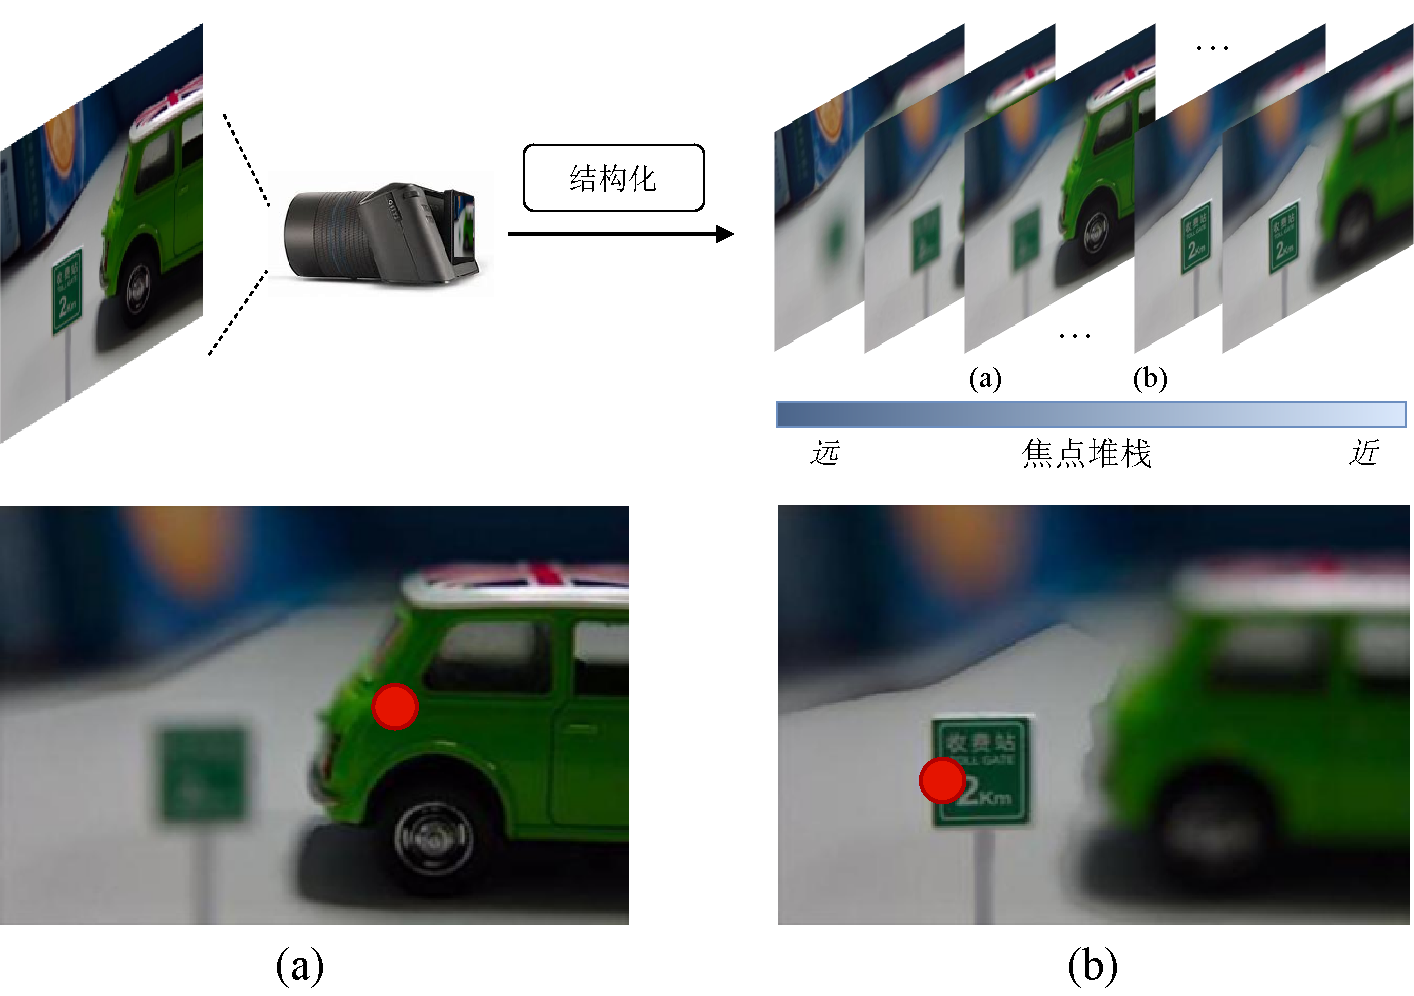
\includegraphics[width=0.85\linewidth]{figures/chapter3/cpt3_idea.pdf}
%	\bicaption{%
%		%		光场焦点堆栈的成像原理和成像效果。
%		%		光场焦点堆栈的成像原理和不同切片的成像效果。
%		光场焦点堆栈的成像过程和不同切片的成像效果。
%		%		\textbf{(a)} 远处视角包含一个清晰的汽车。
%		%		\textbf{(b)} 近处视角包含一个清晰的标志。
%		\textcolor{red}{$\bullet$} 表示清晰的部分。
%		%		焦点堆栈的光场数据结构和焦点堆栈的成像效果的图示。 焦点切片具有随空间透视深度的不同而变化的聚焦部分。
%		%		远处的景色里有一辆清晰的汽车。
%		%		近景画出清晰的标志。
%		%		点表示透明部分。
%	}
%	{ %
%		%			An illustration of the light field data structures to focal stack, and the imaging effect of the focal stack.
%		%			% \textbf{(a)} and \textbf{(b)} indicates that 
%		%			Focal slices have different sharp parts according to the distance from the lens.
%		%			%%
%		%			%%
%		%
%		%% Focal slices have different focusing parts according to the distance from the lens. 
%		%
%		%		An illustration of light field data structures to focal stack and imaging effect of the focal stack. 
%		%		Focal slices have different focusing parts varying with the depth of the spatial perspective.
%		%		The imaging principle and imaging effect of light field focus stack.
%		%		The imaging principle of light field focus stack and the imaging effects of different slices.
%		The imaging process of the light field focus stack and the imaging effects of different slices.
%		%		\textbf{(a)} The distant view contains a clear car.
%		%		\textbf{(b)} The close view draws a clear sign.
%		\textcolor{red}{$\bullet$} indicates the clear parts.  
%	}
%	\label{figure:cpt3:idea}
%\end{figure}
%%
%%


%%------------------------------ figure: comparison
%\begin{figure*}
%	\centering
%	% \setlength{\abovecaptionskip}{-5mm}
%	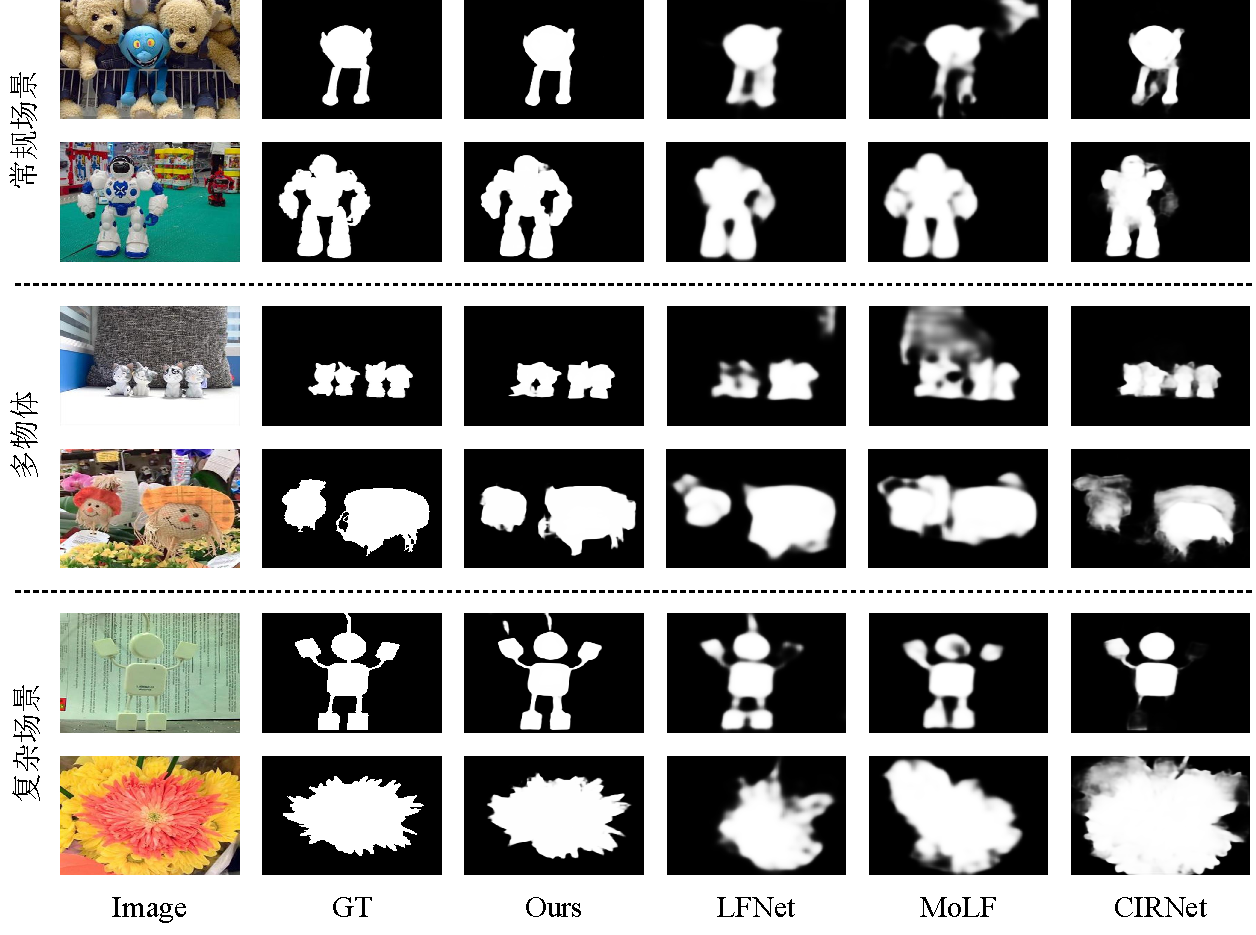
\includegraphics[width=\linewidth]{figures/chapter3/compare_2}
%	%	\caption{
%		%		Qualitative comparisons of state-of-the-art methods in some challenging scenes, including multiple objects and complex scenes.
%		%	}
%	\bicaption{
%		在一些具有挑战性的场景中与最先进的方法的可视化比较。
%	}{
%		Visual comparisons with state-of-the-art methods in challenging scenes.
%		%		Qualitative comparisons of state-of-the-art methods in some challenging scenes, including multiple objects and complex scenes.
%	}
%	\label{figure:figure_comparison_2}
%	\vspace{-0.2cm}
%\end{figure*}
%%
%%

%
%
%	%------------------------------ figure: comparison
%\begin{figure*}
%	\centering
%	% \setlength{\abovecaptionskip}{-5mm}
%	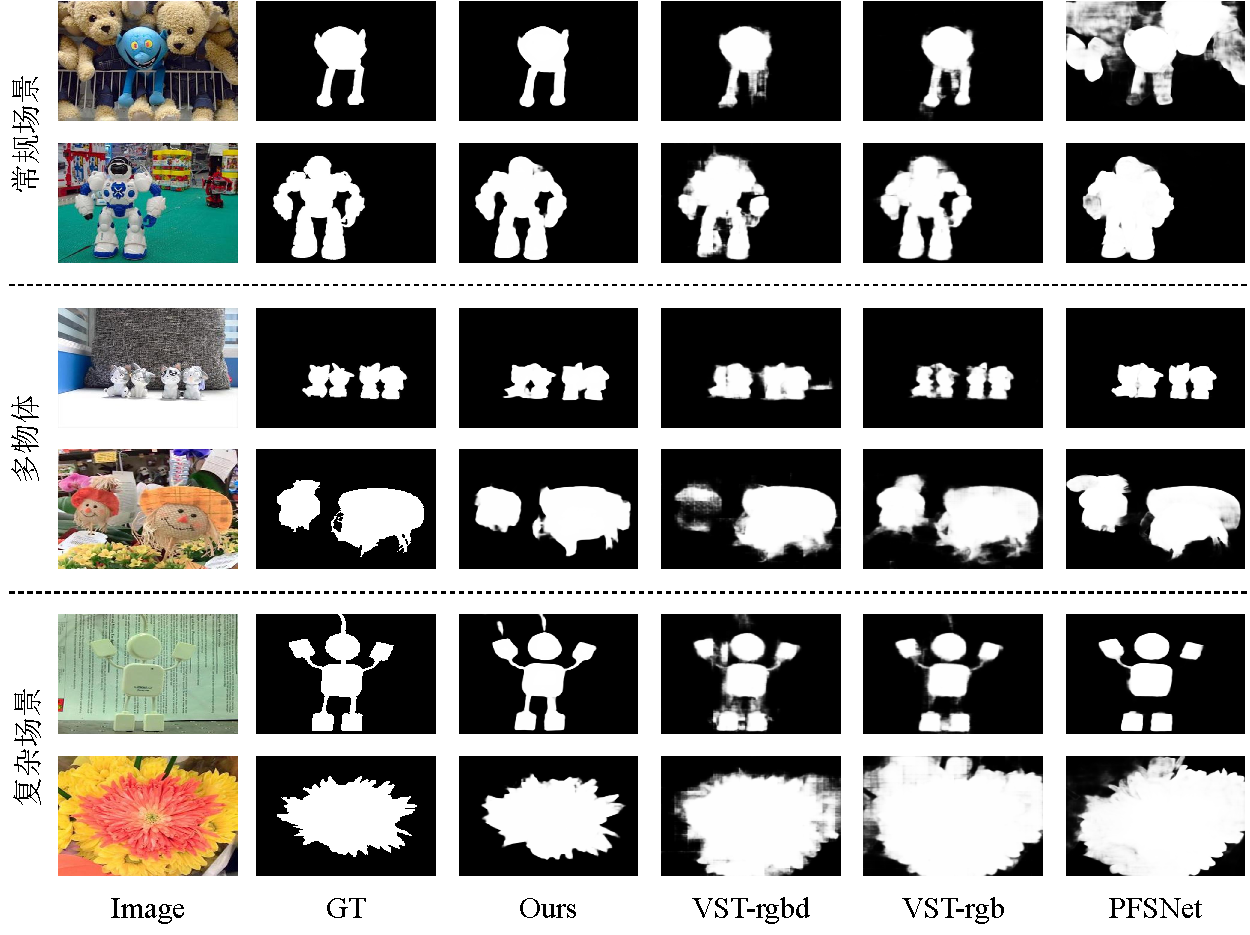
\includegraphics[width=\linewidth]{figures/chapter3/compare_3}
%%	\caption{
	%%		Qualitative comparisons of state-of-the-art methods in some challenging scenes, including multiple objects and complex scenes.
	%%	}
%	\bicaption{
	%		在一些具有挑战性的场景(包括多物体和复杂场景)中对最先进的方法进行定性比较。
	%	}{
	%		Qualitative comparisons of state-of-the-art methods in some challenging scenes, including multiple objects and complex scenes.
	%	}
%	\label{figure:figure_comparison_3}
%	\vspace{-0.2cm}
%\end{figure*}
% 
%



%
%\begin{table}
%	%	\caption{Ablation analyses of each component on the DUTLF-FS dataset.
	%		%		The best results are marked in \textbf{boldface}.
	%		%	}
%	\bicaption{
	%		DUTLF-FS 数据集上每个组件的消融分析。
	%	}{
	%		Ablation analyses of each component on the DUTLF-FS dataset.
	%	}
%	\centering
%	\label{chpt4:tab:abl_2}
%	%	\resizebox{0.82\linewidth}{!}{
	%		\begin{tabular}{llcccc}
		%			\toprule  %添加表格头部粗线
		%			%%  \multicolumn{1}{c}{ \multirow{2}*{Methods} }
		%			
		%			\multicolumn{2}{c}{ \multirow{2}*{Settings}}	& \multicolumn{4}{c}{DUTLF-FS} \\ %& \multicolumn{3}{c}{HFUT} \\ 
		%			
		%			\cmidrule(r){3-6} 
		%			
		%			& & $E_{\phi}^{max}\uparrow$ & $S_{\alpha }\uparrow $ & $F_{\beta}^{max}\uparrow$ & MAE$\downarrow$ \\
		%			\midrule
		%			
		%			% 开始填写数据
		%			\multicolumn{2}{l}{ Baseline }     & 0.947 & 0.894 & 0.901 & 0.048 \\ 
		%			
		%			%		 			\multicolumn{2}{l}{+Token} 	 & 0.959 & 0.918 & 0.926 & 0.037 \\ 
		%			
		%			\midrule
		%			
		%			\multicolumn{1}{c}{ \multirow{2}*{+TCM}}	
		%			
		%			& +TI		& 0.961 & 0.923 & 0.932 & 0.034 \\ 
		%			& ++TS & 0.968 & 0.933 & 0.944 & 0.027 \\
		%			\midrule
		%			
		%			\multicolumn{2}{l}{++FPE} 		& \textbf{0.972} & 0.941 & 0.952 & 0.022 \\
		%			\multicolumn{2}{l}{+++CCM} 		& \textbf{0.972} & \textbf{0.942} & \textbf{0.953} & \textbf{0.021} \\ 
		%			
		%			
		%			\bottomrule
		%		\end{tabular}
	%		% }
%\end{table}
%
%\begin{table}
%	%	\caption{Ablation analyses of each component on the DUTLF-FS dataset.
	%		%		The best results are marked in \textbf{boldface}.
	%		%	}
%	\bicaption{
	%		DUTLF-FS 数据集上每个组件的消融分析。
	%	}{
	%		Ablation analyses of each component on the DUTLF-FS dataset.
	%	}
%	\centering
%	\label{chpt4:tab:abl_3}
%	%	\resizebox{0.82\linewidth}{!}{
	%		\begin{tabular}{llcccc}
		%			\toprule  %添加表格头部粗线
		%			%%  \multicolumn{1}{c}{ \multirow{2}*{Methods} }
		%			
		%			\multicolumn{2}{c}{ \multirow{2}*{Settings}}	& \multicolumn{4}{c}{DUTLF-FS} \\ %& \multicolumn{3}{c}{HFUT} \\ 
		%			
		%			\cmidrule(r){3-6} 
		%			
		%			& & $E_{\phi}^{max}\uparrow$ & $S_{\alpha }\uparrow $ & $F_{\beta}^{max}\uparrow$ & MAE$\downarrow$ \\
		%			\midrule
		%			
		%			% 开始填写数据
		%			\multicolumn{2}{l}{ Baseline }     & 0.947 & 0.894 & 0.901 & 0.048 \\ 
		%			
		%			%		 			\multicolumn{2}{l}{+Token} 	 & 0.959 & 0.918 & 0.926 & 0.037 \\ 
		%			
		%			\midrule
		%			
		%			\multicolumn{1}{c}{ \multirow{2}*{+TCM}}	
		%			
		%			& +TI		& 0.961 & 0.923 & 0.932 & 0.034 \\ 
		%			& ++TS & 0.968 & 0.933 & 0.944 & 0.027 \\
		%			\midrule
		%			
		%			\multicolumn{2}{l}{++FPE} 		& \textbf{0.972} & 0.941 & 0.952 & 0.022 \\
		%			\multicolumn{2}{l}{+++CCM} 		& \textbf{0.972} & \textbf{0.942} & \textbf{0.953} & \textbf{0.021} \\ 
		%			
		%			
		%			\bottomrule
		%		\end{tabular}
	%		% }
%\end{table}




然而,







\todo






大小为原始分别率的

我们的视角增强注意力模块,














% 
% 
在这里,$M_{l-1} \in \left \{  0,1\right \} ^{N \times H_{l}W_{l}} $是前一个
$l-1$层和
\textcolor{red}{TODO}
$M_{0}$是在将查询特征输入Transformer解码器之前,从全聚焦支路获得的二进制掩码预测。
%
%
%
%
\par 
%
%
%











\BiSection{uuu}{uuu}

像素级交叉熵损失。



之后分割头$f_{SEG}$把图像$I$映射到分类激活图
$Y=f_{SEG}(I) \in \mathbb{R}^{H\times H \times |C|}$。
进一步设$y=\left [ y_{1},\dots, y_{C} \right ] \in\mathbb{R}^{C}$
是像素$i$的非归一化得分向量(称为logit),可以从$Y$导出,
即$y \in Y$。
给定像素$i$的真实标签$\bar{c} \in C$,交叉熵使用softmax进行优化:
\begin{equation}
	\mathcal{L}_{i}^{CE}=-1_{\bar{c}}^{\top } log(softmax(y))
	\label{chpt4:eq:loss_softmax}
\end{equation}
% 
% 
% 
% 
其中,$1_{\bar{c}}$表示$\bar{c}$的one-hot编码,
其中的对数算法是逐元素计算的:
\begin{equation}
	softmax(y_{c}) = \frac
	{exp(y_{c})}
	{ 
		\sum_{{c}'=1 }^{|C|} 
		exp(y_{{c}'}) 
	} 
\end{equation}
% 
% 
% 
% 
这种独立训练目标的设计有两个主要限制。
1)它独立的乘法像素级预测,但忽略像素之间的关系~\cite{zhao2019region}。
2)由于使用了softmax,损失仅取决于logits之间的相对关系,
不能直接得到监督学习的表示~\cite{pang2019rethinking}。
这两个问题很少被注意到;只有少数结构感知损失被设计来解决1),
通过考虑像素亲和力~\cite{ke2018adaptive},
优化交叉测量~\cite{berman2018lovasz},
或者最大化真值和预测图之间的互信息~\cite{zhao2019region}。然而,
这些替代损失仅考虑图像内像素之间的依赖性(即全局上下文),
而不考虑图像不同像素之间的语义相关性(即全局结构)
\par
% 
% 
% 
% 

\par
% 
% 


稍后在\todo 和\todo 中提供了定量分析。


像素与区域的对比。
如\todo 所述,记忆是一项关键技术,
有助于对比学习利用海量数据来学习良好的表示。
然而,由于我们的密集预测设置中有大量的像素样本,
并且其中大多数是冗余的(即从相似对象区域采样),
因此像传统存储器一样直接存储所有训练像素样本\todo ,
会大大减慢学习过程。
\par
% 
% 
% 
% 
在队列中维护最后几个批次,例如\todo,
也不是一个最优的选择,
因为最近的批次仅包含有限数量的图像,
降低了像素样本的多样性。
因此,我们选择分别为前景类和背景类维护一个像素队列。
对于每个类别,仅从最新小批量中的每个图像中随机选择少量像素$V$,
并将其拉如队列,大小为$T \gg  V$。
% 
% 
% 
% 
在实践中,我们发现这种策略非常高效并且有效,但是欠采样像素嵌入
太稀疏,无法完全捕获图像内容。
因此,我们进一步构建了一个区域存储库,用于存储从图像片段(即语义区域)
吸收的更具代表性的嵌入。


具体来说,对于总共有$N$个训练图像和$|C|=2$个分割类,
我们的区域内存的大小为$|C|\times N \times D$,
其中$D$是像素嵌入的维度。区域内存中的第$(\bar{c},~n)$
个元素是通过平均池化第n个图像中标记为$c$类别的像素的所有嵌入而获得的
$D$维特征向量。
使用区域内存有两个优点:

1)以较低的内存消耗存储更具代表性的像素样本;
2)允许我们的像素对比损失~\ref{chpt4:eq:con_loss}~进一步探索像素与区域的关系。
关于2),当计算属于$\bar{c}$类别的锚像素$i$时,计算公式~\ref{chpt4:eq:con_loss}~时,
具有相同类别$\bar{c}$的存储区域嵌入被视为正例,
而具有其他类别$C/ \bar{c}$ 的区域嵌入被视为负例。
% 
% 
% 
% 
\par
对于像素存储器,大小为$|C|\times T \times D$。
因此,对于整个内存(记为 $M$ )来说,总大小为$|C| \times (N+T) \times D$。
在\todo 中检查了$M$ 中的像素嵌入和区域嵌入。




\todo 
















%
% 

%
%
%
\par
% 
% 
% 
% 

\par

\par
% 
% 
% 
% 

因此,引入了一种有效的多尺度策略,在控制计算量增加的同时,引入高分辨率特征。
首先,由最高层分辨率特征和下两层较低的分辨率特征组成特征金字塔,
并一次将多尺度的特征的一个分辨率特征传递给一个Transformer解码器层。
\par
% 
% 





Transformer有两个已知的问题。
一是Transformer需要很长的训练时间才能收敛。
假设查询和关键元素的数量分别为$N_{q}$和$N_{k}$,
通过适当的参数初始化,$U_{m}z_{q}$和$ V_{m}x_{k}$遵循均值为0,方差为1的分布,
这使得当$N_{k}$很大时,
注意力权重$A_{mqk} \approx \frac{1}{N_{k}} $。
它将导致输入特征的梯度不明确。
因此,需要很长的训练计划,以便注意力权重可以集中在特定的键上。
在图像领域中,关键元素通常是图像像素,$N_{k}$可能非常大,并且很难收敛。
% 
% 
% 
% 
\par
%
% 
% 
% 
另一方面,由于存在大量查询和关键元素,多头注意力的计算和内存复杂度可能非常高。
方程的计算复杂度为$O\left ( N_{q}C^{2} + N_{k}C^{2}+N_{q}N_{k}C \right ) $。
在图像领域中,查询元素和关键元素都是像素,$N_{q}=N_{k} \gg C$,
复杂度由第三项主导,即$O(N_{q}N_{k}C) $。
因此,多头注意力模块的复杂度随着特征图大小呈二次方增长。


可变形注意力模块。

在图像特征图上应用Transformer的核心问题是让它会查看所有可能得空间位置。
为了解决这个问题,我们采用了一个可变形的注意力模块。
受可变形卷积的启发,
可变形注意力模块仅关注参考点周围的一小组关键采样点,
而不管特征图的空间大小,
通过为每个查询仅分配少量固定数量的键,可以环节收敛和特征空间分辨率的问题。


给定输入特征图$x \in \mathbb{R}^{C\times H \times W}$,
令$q$用作为内容特征$z_{q}$和二维参考点$p_{q}$的索引查询元素,可变性卷积特征
通过以下方式计算,
% 
% 
% 
% 
\begin{equation}
	DeformAttn(z_{q},~p_{q},x)=
	\sum_{m=1}^{M}
	W_{m}\left [ 
	\sum_{k=1}^{K}A_{mqk}~\cdot~
	W_{m}^{'}x\left ( p_{q} + \bigtriangleup p_{mqk} \right ) 
	~~\right ]  
\end{equation}
% 
% 
% 
% 
其中$m$索引注意力头,$k$索引采样键,
$K$是采样键的总数($K \ll HW$),
$\bigtriangleup p_{mqk} $和$A_{mqk}$分别表示
第$m^{th}$个注意力头中第$k^{th}$个采样点的采样偏移量和注意力权重。
标量注意力权重$A_{mqk}$位于$\left [ 0,~1 \right ] $范围内,
通过$ {\textstyle \sum_{k=1}^{K}} A_{mqk}=1$进行归一化。
$\bigtriangleup p_{mqk} \in \mathbb{R}^{2}$
是范围不受约束的二维实数。
由于$p_{q} + \bigtriangleup p_{mqk}$是分数,如等人所述,
$x\left ( p_{q} + \bigtriangleup p_{mqk} \right ) $在计算时应用双线性插值。
$\bigtriangleup p_{mqk}   $和$A_{mqk}$都是通过查询特征$z_{q}$上的线性投影获得的。
在具体实现中,查询特征$z_{q}$被馈送到$3MK$通道的线性投影算子,
其中前$2MK$通道对采样偏移量$\bigtriangleup p_{mqk}$进行编码,
其余$MK$通道通过被馈送到$softmax$算子以获得注意力权重$A_{mqk}$。





可变形注意力模块旨在将卷积特征图作为关键元素进行处理。

设 为查询元素的数量,当较小时,可变形注意力模块的复杂度为。
当应用于DETR编码器时,其中,复杂度变为,
起复杂度与空间大小呈线性关系。
当它作为DETR解码器中的交叉注意力模块应用时,
其中,是对象查询的数量,复杂度变为,
这与空间大小无关。


多尺度可变形注意力模型。
大多数现代目标检测框架都受益于多尺度特征图。
我们提出的可变形注意力模块可以自然地扩展到多尺度特征图。
令为输入多尺度特征图,
其中。
令为每个查询元素的参考点的归一化坐标,
然后应用多尺度可变形注意力采样点。
分别表示第几个特征层和第几个注意力头中第几个采样点的采样偏移和注意力权重。
标量注意力权重通过进行归一化。

这里,为了尺度公式的清晰性,我们使用归一化坐标,
其中归一化坐标分别表示图像的左上角和右下角。
方程中的函数将归一化坐标重新放缩到第几层的输入特征图。


多尺度可变形注意力与之前的单尺度版本非常相似,只是它从多尺度特征图中采样点,
而不是从单尺度特征图中采样k个点。
当且固定为单位矩阵时,所提出的注意力模块将退化为可变形卷积。
可变形卷积是针对单尺度输入而设计的,每个注意力头仅关注一个采样点。
然而,我们的多尺度可变形注意力会关注来自多尺度输入的多个采样点。
所提出的(多尺度)可变形注意模块也可以被视为
Transformer 注意的有效变体,其中通过可变形采样位置引入预过滤机制。
当采样点遍历所有可能得位置时,所提出的注意力模块相当于Transformer注意力。


可变形Transformer 编码器。

我们将网络中处理特征图的Transformer注意模块替换为所提出的多尺度可变形注意模块。
编码器的输入和输出都是具有相同分辨率的多尺度特征图。

在编码器中,我们从骨干网络中提取多尺度特征图,通过卷积,
其中的分辨率比输入图像低。
最低分辨率特征图是通过最后阶段的步长卷积获得的。

所有多尺度特征图均为个通道,
像FPN网络结构中,没有使用自上而下的结构,因为我们提出的多尺度可变形注意力本身可以在多尺度特征图之间交换信息。






%
%\begin{table*}[]
%	%
%	%---------------------------------------------------------------------> 大表 
%	%
%	\caption{Quantitative comparison of our proposed FPT with other 20 SOTA SOD methods on three benchmark datasets. 
	%		$ \uparrow \& \downarrow $ denote larger and smaller is better.
	%		%
	%		% denote the best and the second-best results,
	%		%
	%		The best three results are shown in 
	%		\textbf{boldface}, \textcolor{red}{red} and \textcolor{blue}{blue} fonts respectively. 
	%		% '-' indicates the code or outcome is not available.
	%	}
%	\centering
%	\label{table:comp_with_sota_1}
%%	\resizebox{\textwidth}{!}{
	%		\begin{tabular}{crcccc}
		%			\toprule  %添加表格头部粗线
		%			
		%			% title
		%			\multirow{2}*{Type} & \multicolumn{1}{c}{ \multirow{2}*{Methods} } & 
		%			\multicolumn{4}{c}{DUTLF-FS \cite{zhang2019memory} } \\
		%
		%			
		%			% next line
		%			\cmidrule(r){3-6} 
		%			
		%			% subtitle
		%			& & 
		%			$E_{\phi}^{max}\uparrow$ & $S_{\alpha }\uparrow$ & $F_{\beta}^{max}\uparrow$ & MAE$\downarrow$ \\
		%		
		%			
		%			% line line
		%			\midrule
		%			
		%			\multirow{8}*{\textit{Light field}}
		%			
		%			% 开始填数据
		%			
		%			& Ours	 &  {\textbf{0.973}} & \textbf{ {0.946}} 
		%			& \textbf{ {0.954}} & \textbf{ {0.020}} 
		%			\\
		%			
		%			& DLGLRG \cite{liu2021light} 
		%			& {\textcolor{red}{0.958}} & {\textcolor{red}{0.928}} 
		%			& {\textcolor{red}{0.934}} & {\textcolor{red}{0.029}} 
		%			\\
		%			
		%			& ERNet \cite{piao2020exploit}
		%			& 0.947 & 0.899 & 0.908 & 0.039  \\
		%			
		%			& PANet \cite{piao2021panet} 
		%			% & 0.9390 & 0.9080 & 0.9029 & 0.0383 & 0.8449 & 0.7949 & 0.7383 & 0.0743 & 0.8922 & 0.8487 & 0.8494 & 0.0761 
		%			& 0.939 & 0.908 & 0.903 & 0.038
		%			\\
		%			
		%			& LFNet	 \cite{zhang2020lfnet} 
		%			& 0.929 & 0.878 & 0.890 & 0.053 	 \\
		%			
		%			& MAC	 \cite{zhang2020light} 
		%			& 0.863	& 0.804	& 0.792	& 0.102	    \\
		%			
		%			& MoLF	 \cite{zhang2019memory} 
		%			& 0.938 & 0.887 & 0.902 & 0.051 	 \\
		%			
		%			& DLSD	\cite{piao2019deep}
		%			& 0.891	& 0.841	& 0.801	& 0.076	    \\
		%			
		%			\midrule % end lfsod
		%			
		%			% start rgb-d
		%			\multirow{6}*{\textit{RGB-D}}
		%			
		%			% & 001& Male & 001& Male& 001& Male& 001& Male& 001& Male & 001& Male  & 001& Male \\
		%			
		%			& DCF \cite{ji2021calibrated} 
		%			& \textcolor{blue}{0.954} & \textcolor{blue}{0.921} & \textcolor{blue}{0.927} & \textcolor{blue}{0.031} 
		%		 	\\
		%			
		%			& CIR-Net \cite{cong2022cir}
		%			& 0.950 & 0.916 & 0.921 & 0.038 
		%		    \\ 
		%			
		%			& VST-$rgbd$  \cite{liu2021visual} 
		%			& 0.952 & 0.920 & 0.921 & 0.036 
		%			\\
		%			
		%			
		%			& BBS-Net     \cite{fan2020bbs} 
		%			& 0.900 & 0.865 & 0.852 & 0.066 
		%			\\ 
		%			
		%			& SSF     \cite{zhang2020select} 
		%			& 0.922 & 0.879 & 0.887 & 0.050 
		%			\\ 
		%			
		%			& S2MA    \cite{liu2020learning} 
		%			& 0.839 & 0.787 & 0.754 & 	0.102 
		%			\\
		%			
		%			\midrule % end rgb-d
		%			
		%			\multirow{7}*{\textit{RGB}}
		%			
		%			& VST-$rgb$ \cite{liu2021visual} 
		%			& 0.939 & 0.910 & 0.911 & 0.047  \\ 
		%			
		%			& PFSNet \cite{ma2021pyramidal}
		%			& 0.912 & 0.883 & 0.879 & 0.057  \\ 
		%			
		%			& ITSD \cite{zhou2020interactive} & 
		%			0.930 & 0.899 & 0.899 & 0.052  \\ 
		%			
		%			
		%			
		%			& LDF \cite{wei2020label} &
		%			0.898 & 0.873 & 0.861 & 0.061 \\ 
		%			
		%			
		%			& MINet \cite{pang2020multi} &
		%			0.916 & 0.890 & 0.882 & 0.050  \\ 
		%			
		%			& F$^{3}$Net  \cite{wei2020f3net}
		%			& 0.900 & 0.888 & 0.882 & 0.057  \\ 
		%			
		%			& EGNet   \cite{zhao2019egnet}
		%			& 0.914 & 0.886 & 0.870 & 0.053 \\ 
		%			
		%			\bottomrule % end
		%	\end{tabular}
	%%}
%\end{table*}
%
%
%
%\begin{table*}[]
%	%
%	%---------------------------------------------------------------------> 大表 
%	%
%	\caption{Quantitative comparison of our proposed FPT with other 20 SOTA SOD methods on three benchmark datasets. 
	%		$ \uparrow \& \downarrow $ denote larger and smaller is better.
	%		%
	%		% denote the best and the second-best results,
	%		%
	%		The best three results are shown in 
	%		\textbf{boldface}, \textcolor{red}{red} and \textcolor{blue}{blue} fonts respectively. 
	%		% '-' indicates the code or outcome is not available.
	%	}
%	\centering
%	\label{table:comp_with_sota_2}
%%	\label{table:comp-with-sota}
%%	\resizebox{\textwidth}{!}{
	%		\begin{tabular}{crcccc}
		%			\toprule  %添加表格头部粗线
		%			
		%			% title
		%			\multirow{2}*{Type} & \multicolumn{1}{c}{ \multirow{2}*{Methods} } & 
		%			\multicolumn{4}{c}{HFUT \cite{zhang2017saliency} } \\
		%			
		%			% next line
		%			\cmidrule(r){3-6} 
		%			
		%			% subtitle
		%			& & 
		%			$E_{\phi}^{max}\uparrow$ & $S_{\alpha }\uparrow$ & $F_{\beta}^{max}\uparrow$ & MAE$\downarrow$ \\
		%			
		%			% line line
		%			\midrule
		%			
		%			\multirow{8}*{\textit{Light field}}
		%			
		%			% 开始填数据
		%			
		%			& Ours	 
		%			& \textbf{ {0.871}} &	\textbf{ {0.828}} 
		%			&\textbf{	 {0.784}} & {\textcolor{red}{0.064}} 
		%		    \\
		%			
		%			& DLGLRG \cite{liu2021light} 
		%			&	0.839 &	0.766 &	0.698 &	0.070 
		%	        \\
		%			
		%			& ERNet \cite{piao2020exploit}
		%			&	0.841 &	0.778 &	0.722 &	0.082 \\
		%			
		%			& PANet \cite{piao2021panet} 
		%			% & 0.9390 & 0.9080 & 0.9029 & 0.0383 & 0.8449 & 0.7949 & 0.7383 & 0.0743 & 0.8922 & 0.8487 & 0.8494 & 0.0761 
		%			& 0.845 & 0.795 & 0.738 & 0.074 
		%			\\
		%			
		%			& LFNet	 \cite{zhang2020lfnet} 
		%			&	0.846 &	0.782 &	0.718 &	0.073 \\
		%			
		%			& MAC	 \cite{zhang2020light} 
		%			&   0.797 & 0.731 & 0.667 & 0.107 
		%			\\
		%			
		%			& MoLF	 \cite{zhang2019memory} 
		%			&	0.852 &	0.789 &	0.729 &	0.075 \\
		%			
		%			& DLSD	\cite{piao2019deep}
		%			&   0.783 & 0.741 & 0.615 & 0.098 \\
		%			
		%			
		%			\midrule % end lfsod
		%			
		%			\multirow{6}*{\textit{RGB-D}}
		%
		%			
		%			& DCF \cite{ji2021calibrated} 
		%			& \textcolor{blue}{0.856} & {\textcolor{red}{0.812}} & {\textcolor{red}{0.768}} & \textcolor{blue}{0.065} 
		%			\\
		%			
		%			& CIR-Net \cite{cong2022cir}
		%			& {\textcolor{red}{0.862}} & 0.800 
		%			& 0.742 & \textbf{ {0.062}} 
		%			\\ 
		%			
		%			& VST-$rgbd$  \cite{liu2021visual} 
		%			& 0.843 & 0.807 & 0.754 & 0.086  \\
		%
		%			
		%			& BBS-Net     \cite{fan2020bbs} 
		%			& 0.801 & 0.751 & 0.676 & 0.073 
		%			\\ 
		%			
		%			& SSF     \cite{zhang2020select} 
		%			& 0.816 & 0.725 & 0.647 & 0.090 
		%		    \\ 
		%			
		%			& S2MA    \cite{liu2020learning} 
		%		    & 0.777 & 0.729 & 0.650 & 0.112 \\
		%			
		%			
		%			%			& TriTransNet	&  & \\
		%			%			& DCFNet  & \\
		%			
		%			\midrule % end rgb-d
		%			
		%			% start rgb sod
		%			\multirow{7}*{\textit{RGB}}
		%			
		%			& VST-$rgb$ \cite{liu2021visual} 
		%			& 0.831 & \textcolor{blue}{0.808} & \textcolor{blue}{0.763} & 0.093 \\ 
		%			
		%			& PFSNet \cite{ma2021pyramidal}
		%			&  0.835 & 0.800 & 0.752 & 0.088  \\ 
		%			
		%			%			& - & \\
		%			
		%			& ITSD \cite{zhou2020interactive} & 
		%			 0.839 & 0.805 & 0.759 & 0.089  \\ 
		%			
		%			
		%			
		%			& LDF \cite{wei2020label} &
		%			 0.804 & 0.780 & 0.708 & 0.093  \\ 
		%			
		%			
		%			& MINet \cite{pang2020multi} 
		%			 & 0.816 & 0.792 & 0.720 & 0.086  \\ 
		%			
		%			& F$^{3}$Net  \cite{wei2020f3net}
		%			& 0.815 & 0.777 & 0.718 & 0.095  \\ 
		%
		%			
		%			& EGNet   \cite{zhao2019egnet}
		%			 & 0.794 & 0.772 & 0.672 & 0.094  \\ 
		%			
		%			\bottomrule % end
		%	\end{tabular}
	%%}
%\end{table*}


%
%\begin{table*}[]
%	%
%	%---------------------------------------------------------------------> 大表 
%	%
%	\caption{Quantitative comparison of our proposed FPT with other 20 SOTA SOD methods on three benchmark datasets. 
	%		$ \uparrow \& \downarrow $ denote larger and smaller is better.
	%		%
	%		% denote the best and the second-best results,
	%		%
	%		The best three results are shown in 
	%		\textbf{boldface}, \textcolor{red}{red} and \textcolor{blue}{blue} fonts respectively. 
	%		% '-' indicates the code or outcome is not available.
	%	}
%	\centering
%	\label{table:comp_with_sota_3}
%%	\label{table:comp-with-sota}
%%	\resizebox{\textwidth}{!}{
	%		\begin{tabular}{crcccc}
		%			\toprule  %添加表格头部粗线
		%			
		%%			\multirow{2}*{Type} & 
		%			\multicolumn{1}{c}{ \multirow{2}*{Methods} } & 
		%			% \multirow{2}*{Years} &
		%			% \multicolumn{1}{c}{Type} & \multicolumn{1}{c}{Methods} & \multicolumn{1}{c}{Years} & 
		%			\multicolumn{4}{c}{DUTLF-FS \cite{zhang2019memory} } &
		%			\multicolumn{4}{c}{HFUT \cite{zhang2017saliency} } &
		%			\multicolumn{4}{c}{LFSD \cite{li2014saliency} } \\
		%			
		%			% next line
		%			\cmidrule(r){2-5} \cmidrule(r){6-9} \cmidrule(r){10-13}
		%			
		%			% subtitle
		%			& 
		%			$E_{\phi}^{max}\uparrow$ & $S_{\alpha }\uparrow$ & $F_{\beta}^{max}\uparrow$ & MAE$\downarrow$ &
		%			$E_{\phi}^{max}\uparrow$ & $S_{\alpha }\uparrow$ & $F_{\beta}^{max}\uparrow$ & MAE$\downarrow$  &
		%			$E_{\phi}^{max}\uparrow$ & $S_{\alpha }\uparrow$ & $F_{\beta}^{max}\uparrow$ & MAE$\downarrow$ \\
		%			
		%			
		%			% line line
		%			\midrule
		%			
		%			\multirow{8}*{\textit{Light field}}
		%			
		%			% 开始填数据
		%			
		%			& Ours	 
		%%			&  {\textbf{0.973}} & \textbf{ {0.946}} 	& \textbf{ {0.954}} & \textbf{ {0.020}} 
		%%			& \textbf{ {0.871}} &	\textbf{ {0.828}} 			&\textbf{	 {0.784}} & {\textcolor{red}{0.064}} 
		%			& \textbf{ {0.919}} &	\textcolor{blue}{0.860} 			&	\textbf{ {0.873}} &	\textbf{ {0.064}} 
		%			\\
		%			
		%			& DLGLRG \cite{liu2021light} 
		%%			& {\textcolor{red}{0.958}} & {\textcolor{red}{0.928}} 			& {\textcolor{red}{0.934}} & {\textcolor{red}{0.029}} 
		%%			&	0.839 &	0.766 &	0.698 &	0.070 
		%			&	{\textcolor{red}{0.906}} &	\textbf{ {0.866}} 			&	{\textcolor{red}{0.870}} &	\textcolor{blue}{0.069} 
		%			\\
		%			
		%			& ERNet \cite{piao2020exploit}
		%%			& 0.947 & 0.899 & 0.908 & 0.039 
		%%			&	0.841 &	0.778 &	0.722 &	0.082 
		%			&	0.888 &	0.834 &	0.850 &	0.082 
		%			\\
		%			
		%			& PANet \cite{piao2021panet} 
		%%			& 0.939 & 0.908 & 0.903 & 0.038 
		%%			& 0.845 & 0.795 & 0.738 & 0.074 
		%			& 0.892 & 0.849 & 0.849 & 0.076
		%			\\
		%			
		%			& LFNet	 \cite{zhang2020lfnet} 
		%%			& 0.929 & 0.878 & 0.890 & 0.053
		%%			 &	0.846 &	0.782 &	0.718 &	0.073 
		%			 &	0.885 &	0.820 &	0.824 &	0.092 \\
		%			
		%			& MAC	 \cite{zhang2020light} 
		%%			& 0.863	& 0.804	& 0.792	& 0.102	
		%%			&   0.797 & 0.731 & 0.667 & 0.107 
		%			& 0.832 & 0.782 & 0.776 & 0.127 \\
		%			
		%			& MoLF	 \cite{zhang2019memory} 
		%%			& 0.938 & 0.887 & 0.902 & 0.051 
		%%			&	0.852 &	0.789 &	0.729 &	0.075 
		%			&	0.888 &	0.830 &	0.834 &	0.089 \\
		%			
		%			& DLSD	\cite{piao2019deep}
		%%			& 0.891	& 0.841	& 0.801	& 0.076	
		%%			&   0.783 & 0.741 & 0.615 & 0.098 
		%			& 0.806 & 0.737 & 0.715 & 0.147 \\
		%			
		%			\midrule % end lfsod
		%			
		%			% start rgb-d
		%			\multirow{6}*{\textit{RGB-D}}
		%			
		%			& DCF \cite{ji2021calibrated} 
		%%			& \textcolor{blue}{0.954} & \textcolor{blue}{0.921} & \textcolor{blue}{0.927} & \textcolor{blue}{0.031} 
		%%			& \textcolor{blue}{0.856} & {\textcolor{red}{0.812}} & {\textcolor{red}{0.768}} & \textcolor{blue}{0.065} 
		%			& 0.881 & 0.809 & 0.821 & 0.096 \\
		%			
		%			& CIR-Net \cite{cong2022cir}
		%%			& 0.950 & 0.916 & 0.921 & 0.038 
		%%			& {\textcolor{red}{0.862}} & 0.800  			& 0.742 & \textbf{ {0.062}} 
		%			& 0.874 & 0.820 & 0.816 & 0.098 \\ 
		%			
		%			& VST-$rgbd$  \cite{liu2021visual} 
		%%			& 0.952 & 0.920 & 0.921 & 0.036 
		%%			& 0.843 & 0.807 & 0.754 & 0.086 
		%			& 0.851 & 0.792 & 0.786 & 0.110 
		%			\\
		%			
		%			%			& -  & 2022  & \\
		%			%			& -  & 2022  & \\
		%			
		%			& BBS-Net     \cite{fan2020bbs} 
		%%			& 0.900 & 0.865 & 0.852 & 0.066 
		%%			& 0.801 & 0.751 & 0.676 & 0.073 
		%			& \textcolor{blue}{0.901} & {\textcolor{red}{0.864}} & 0.858 & 0.072 \\ 
		%			
		%			& SSF     \cite{zhang2020select} 
		%%			& 0.922 & 0.879 & 0.887 & 0.050 
		%%			& 0.816 & 0.725 & 0.647 & 0.090 
		%			& \textcolor{blue}{0.901} & 0.859 & \textcolor{blue}{0.868} & {\textcolor{red}{0.067}} \\ 
		%			
		%			& S2MA    \cite{liu2020learning} 
		%%			& 0.839 & 0.787 & 0.754 & 	0.102 
		%%			& 0.777 & 0.729 & 0.650 & 0.112 
		%			& 0.873 & 0.837 &	0.835 & 0.094 \\
		%
		%			
		%			\midrule % end rgb-d
		%			\multirow{7}*{\textit{RGB}}
		%			
		%			& VST-$rgb$ \cite{liu2021visual} 
		%%			& 0.939 & 0.910 & 0.911 & 0.047
		%%			& 0.831 & \textcolor{blue}{0.808} & \textcolor{blue}{0.763} & 0.093 
		%			& 0.865 & 0.797 & 0.817 & 0.123 
		%			\\ 
		%			
		%			& PFSNet \cite{ma2021pyramidal}
		%%			& 0.912 & 0.883 & 0.879 & 0.057 
		%%			& 0.835 & 0.800 & 0.752 & 0.088 
		%			& 0.805 & 0.749 & 0.727 & 0.145 
		%			\\ 
		%
		%			
		%			& ITSD \cite{zhou2020interactive} 
		%%			& 0.930 & 0.899 & 0.899 & 0.052 
		%%			& 0.839 & 0.805 & 0.759 & 0.089 
		%			& 0.879 & 0.847 & 0.840 & 0.088 
		%			\\ 
		%			
		%			
		%			
		%			& LDF \cite{wei2020label} 
		%%			& 0.898 & 0.873 & 0.861 & 0.061 
		%%			& 0.804 & 0.780 & 0.708 & 0.093 
		%			& 0.843 & 0.821 & 0.803 & 0.096 
		%			\\ 
		%			
		%			
		%			& MINet \cite{pang2020multi} 
		%%			& 0.916 & 0.890 & 0.882 & 0.050 
		%%			& 0.816 & 0.792 & 0.720 & 0.086 
		%			& 0.861 & 0.834 & 0.828 & 0.091 
		%			\\ 
		%			
		%			& F$^{3}$Net  \cite{wei2020f3net}
		%%			& 0.900 & 0.888 & 0.882 & 0.057 
		%%			& 0.815 & 0.777 & 0.718 & 0.095 
		%			& 0.824 & 0.806 & 0.797 & 0.106 
		%			\\ 
		%			
		%			
		%			& EGNet   \cite{zhao2019egnet}
		%%			& 0.914 & 0.886 & 0.870 & 0.053 
		%%			& 0.794 & 0.772 & 0.672 & 0.094 
		%			& 0.776 & 0.784 & 0.762 & 0.118 
		%			\\ 
		%			
		%			\bottomrule % end
		%	\end{tabular}
	%%}
%\end{table*}




%
%\begin{table*}[]
%	%
%	%---------------------------------------------------------------------> 大表 
%	%
%	\caption{Quantitative comparison of our proposed FPT with other 20 SOTA SOD methods on three benchmark datasets. 
	%		$ \uparrow \& \downarrow $ denote larger and smaller is better.
	%		%
	%		% denote the best and the second-best results,
	%		%
	%		The best three results are shown in 
	%		\textbf{boldface}, \textcolor{red}{red} and \textcolor{blue}{blue} fonts respectively. 
	%		% '-' indicates the code or outcome is not available.
	%	}
%	\centering
%	\label{table:comp_with_sota_3}
%	%	\label{table:comp-with-sota}
%		\resizebox{\textwidth}{!}{
	%		\begin{tabular}{rcccccccccccc}
		%			\toprule  %添加表格头部粗线
		%			
		%			% title
		%%			\multirow{2}*{Type} & 
		%			\multicolumn{1}{c}{ \multirow{2}*{Methods} } & 
		%			\multicolumn{4}{c}{DUTLF-FS \cite{zhang2019memory} } &
		%			\multicolumn{4}{c}{HFUT \cite{zhang2017saliency} } &
		%			\multicolumn{4}{c}{LFSD \cite{li2014saliency} } \\
		%			
		%			% next line
		%			\cmidrule(r){2-5} \cmidrule(r){6-9} \cmidrule(r){10-13}
		%			
		%			% subtitle
		%			& 
		%			$E_{\phi}^{max}\uparrow$ & $S_{\alpha }\uparrow$ & $F_{\beta}^{max}\uparrow$ & MAE$\downarrow$ &
		%			$E_{\phi}^{max}\uparrow$ & $S_{\alpha }\uparrow$ & $F_{\beta}^{max}\uparrow$ & MAE$\downarrow$  &
		%			$E_{\phi}^{max}\uparrow$ & $S_{\alpha }\uparrow$ & $F_{\beta}^{max}\uparrow$ & MAE$\downarrow$ \\
		%			
		%			
		%			
		%			% line line
		%			\midrule
		%			
		%%			\multirow{8}*{\textit{Light field}}
		%			
		%			% 开始填数据
		%			
		%			 Ours	 
		%						&  {\textbf{0.973}} & \textbf{ {0.946}} 	& \textbf{ {0.954}} & \textbf{ {0.020}} 
		%						& \textbf{ {0.871}} &	\textbf{ {0.828}} 			&\textbf{	 {0.784}} & {\textcolor{red}{0.064}} 
		%			& \textbf{ {0.919}} &	\textcolor{blue}{0.860} 			&	\textbf{ {0.873}} &	\textbf{ {0.064}} 
		%			\\
		%			
		%			 DLGLRG \cite{liu2021light} 
		%						& {\textcolor{red}{0.958}} & {\textcolor{red}{0.928}} 			& {\textcolor{red}{0.934}} & {\textcolor{red}{0.029}} 
		%						&	0.839 &	0.766 &	0.698 &	0.070 
		%			&	{\textcolor{red}{0.906}} &	\textbf{ {0.866}} 			&	{\textcolor{red}{0.870}} &	\textcolor{blue}{0.069} 
		%			\\
		%			
		%			 ERNet \cite{piao2020exploit}
		%						& 0.947 & 0.899 & 0.908 & 0.039 
		%						&	0.841 &	0.778 &	0.722 &	0.082 
		%			&	0.888 &	0.834 &	0.850 &	0.082 
		%			\\
		%			
		%			 PANet \cite{piao2021panet} 
		%						& 0.939 & 0.908 & 0.903 & 0.038 
		%						& 0.845 & 0.795 & 0.738 & 0.074 
		%			& 0.892 & 0.849 & 0.849 & 0.076
		%			\\
		%			
		%			 LFNet	 \cite{zhang2020lfnet} 
		%						& 0.929 & 0.878 & 0.890 & 0.053
		%						 &	0.846 &	0.782 &	0.718 &	0.073 
		%			&	0.885 &	0.820 &	0.824 &	0.092 \\
		%			
		%			 MAC	 \cite{zhang2020light} 
		%						& 0.863	& 0.804	& 0.792	& 0.102	
		%						&   0.797 & 0.731 & 0.667 & 0.107 
		%			& 0.832 & 0.782 & 0.776 & 0.127 \\
		%			
		%			 MoLF	 \cite{zhang2019memory} 
		%						& 0.938 & 0.887 & 0.902 & 0.051 
		%						&	0.852 &	0.789 &	0.729 &	0.075 
		%			&	0.888 &	0.830 &	0.834 &	0.089 \\
		%			
		%			 DLSD	\cite{piao2019deep}
		%						& 0.891	& 0.841	& 0.801	& 0.076	
		%						&   0.783 & 0.741 & 0.615 & 0.098 
		%			& 0.806 & 0.737 & 0.715 & 0.147 \\
		%			
		%			\midrule % end lfsod
		%			
		%			% start rgb-d
		%%			\multirow{6}*{\textit{RGB-D}}
		%			
		%			 DCF \cite{ji2021calibrated} 
		%						& \textcolor{blue}{0.954} & \textcolor{blue}{0.921} & \textcolor{blue}{0.927} & \textcolor{blue}{0.031} 
		%						& \textcolor{blue}{0.856} & {\textcolor{red}{0.812}} & {\textcolor{red}{0.768}} & \textcolor{blue}{0.065} 
		%			& 0.881 & 0.809 & 0.821 & 0.096 \\
		%			
		%			 CIR-Net \cite{cong2022cir}
		%						& 0.950 & 0.916 & 0.921 & 0.038 
		%						& {\textcolor{red}{0.862}} & 0.800  			& 0.742 & \textbf{ {0.062}} 
		%			& 0.874 & 0.820 & 0.816 & 0.098 \\ 
		%			
		%		 VST-$rgbd$  \cite{liu2021visual} 
		%						& 0.952 & 0.920 & 0.921 & 0.036 
		%						& 0.843 & 0.807 & 0.754 & 0.086 
		%			& 0.851 & 0.792 & 0.786 & 0.110 
		%			\\
		%			
		%			%			& -  & 2022  & \\
		%			%			& -  & 2022  & \\
		%			
		%			 BBS-Net     \cite{fan2020bbs} 
		%						& 0.900 & 0.865 & 0.852 & 0.066 
		%						& 0.801 & 0.751 & 0.676 & 0.073 
		%			& \textcolor{blue}{0.901} & {\textcolor{red}{0.864}} & 0.858 & 0.072 \\ 
		%			
		%			 SSF     \cite{zhang2020select} 
		%						& 0.922 & 0.879 & 0.887 & 0.050 
		%						& 0.816 & 0.725 & 0.647 & 0.090 
		%			& \textcolor{blue}{0.901} & 0.859 & \textcolor{blue}{0.868} & {\textcolor{red}{0.067}} \\ 
		%			
		%			 S2MA    \cite{liu2020learning} 
		%						& 0.839 & 0.787 & 0.754 & 	0.102 
		%						& 0.777 & 0.729 & 0.650 & 0.112 
		%			& 0.873 & 0.837 &	0.835 & 0.094 \\
		%			
		%			
		%			\midrule % end rgb-d
		%%			\multirow{7}*{\textit{RGB}}
		%			
		%			 VST-$rgb$ \cite{liu2021visual} 
		%						& 0.939 & 0.910 & 0.911 & 0.047
		%						& 0.831 & \textcolor{blue}{0.808} & \textcolor{blue}{0.763} & 0.093 
		%			& 0.865 & 0.797 & 0.817 & 0.123 
		%			\\ 
		%			
		%			 PFSNet \cite{ma2021pyramidal}
		%						& 0.912 & 0.883 & 0.879 & 0.057 
		%						& 0.835 & 0.800 & 0.752 & 0.088 
		%			& 0.805 & 0.749 & 0.727 & 0.145 
		%			\\ 
		%			
		%			
		%			 ITSD \cite{zhou2020interactive} 
		%						& 0.930 & 0.899 & 0.899 & 0.052 
		%						& 0.839 & 0.805 & 0.759 & 0.089 
		%			& 0.879 & 0.847 & 0.840 & 0.088 
		%			\\ 
		%			
		%			
		%			
		%			LDF \cite{wei2020label} 
		%						& 0.898 & 0.873 & 0.861 & 0.061 
		%						& 0.804 & 0.780 & 0.708 & 0.093 
		%			& 0.843 & 0.821 & 0.803 & 0.096 
		%			\\ 
		%			
		%			
		%			MINet \cite{pang2020multi} 
		%						& 0.916 & 0.890 & 0.882 & 0.050 
		%						& 0.816 & 0.792 & 0.720 & 0.086 
		%			& 0.861 & 0.834 & 0.828 & 0.091 
		%			\\ 
		%			
		%			F$^{3}$Net  \cite{wei2020f3net}
		%						& 0.900 & 0.888 & 0.882 & 0.057 
		%						& 0.815 & 0.777 & 0.718 & 0.095 
		%			& 0.824 & 0.806 & 0.797 & 0.106 
		%			\\ 
		%			
		%			
		%			EGNet   \cite{zhao2019egnet}
		%						& 0.914 & 0.886 & 0.870 & 0.053 
		%						& 0.794 & 0.772 & 0.672 & 0.094 
		%			& 0.776 & 0.784 & 0.762 & 0.118 
		%			\\ 
		%			
		%			\bottomrule % end
		%		\end{tabular}
	%		}
%\end{table*}


% %%==================================================
%% chapter01.tex for DUT Thesis 
%% version: 0.1
%% last update: Dec 25th, 2022
%%==================================================
\BiChapter{绪论}{Introduction}
绪论应包括本研究课题的学术背景及其理论与实际意义;本领域的国内外研究进展及成果、存在不足或有待深入研究的问题;本研究课题的来源及主要研究内容等。
\label{chap:intro}
\BiSection{研究背景与意义}{Research background}

\BiSection{国内外相关研究工作进展}{Research progress}

\BiSection{论文研究思路及目标}{Main research contents and objectives}





% \BiChapter{Latex模板简介}{The Introduction of Latex Template}
本章介绍Latex的文本控制流程,介绍学位论文中各章节分布及模板内部组成,用户可根据自身对Latex的熟悉程度适当地略过阅读。\par
\BiSection{认识模板组成}{Understanding Template Composition}
格式控制文件控制着论文的表现形式,包括以下两个后缀的文件:“.cls”后缀的文件控制论文主体格式和“.bst”后缀的文件控制参考文献条目。\par
一般用户在.cls后缀的文件里填写封面、申明和授权书及奇偶页页眉内容,然后在各章正文处进行内容的填写。
\BiSection{主控文件}{Main File}
主控文件MA Thesis.tex的作用就是将分散在多个文件中的内容整合成一篇完整的内容。此部分用户不需做改动。
\BiSection{论文主体文件夹chapters}{Chapters File}
这一部分是论文的主体,是以“章”为单位划分的。用户需要在这里对中英文摘要、符号表、各章内容、附录、致谢、攻读学位论文期间的成果及作者简介进行填写。
\BiSection{图片文件夹figures}{Figures File}
figures文件夹放置了需要插入文档中的图片文件(PNG/JPG/PDF/EPS)。如果图片较多,建议按章再划分子目录存储图片。
\BiSection{参考文献数据库文件夹reference}{Reference File}
此文件夹用于存放参考文献信息。bib数据库中的参考文献条目可以手动编写,也可以在Google的学术搜索中找到。各大数据库也支持将参考文献信息导出为.bib。
\BiSection{本章小结}{The Chapter’s Conclusion}




% \BiChapter{图表、公式、代码及参考文献的编制方法}{The Compile Method of Chart, Formula , Code and Reference }
\BiSection{向文档中插入图像}{Inserts an Image Into the Document}
\BiSubsection{单张图片的插入}{Insertion of a Single Image}
在学位论文中,可插入PDF、EPS、PNG、JPG格式的图片。以图3.1的插入为例,插入代码为3.1所示,其中\textbackslash centering表示图片居中,\textbackslash includegraphics[...]\{...\}导入图片并定制图片大小,\textbackslash\{...\}指定图片标题,而\textbackslash lable\{...\}为图片加上引用标签:
\begin{lstlisting}[caption={示例插图代码}]
\begin{figure}[!ht]
\centering
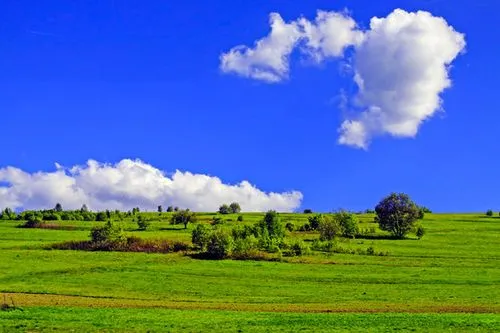
\includegraphics{figures/figure4}
\bicaption{图片}{Picture}  \label{fig4:diagram}
\end{figure}
\end{lstlisting}

\begin{figure}[!ht]
	\centering
	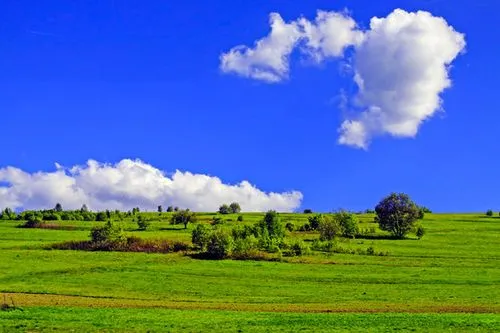
\includegraphics{figures/figure4}
	\bicaption{图片}{Picture}  \label{fig4:diagram}
\end{figure}
\BiSubsection{两张并列图片的插入}{The Insertion of Two Side-by-side Pictures}
插入两幅并列子图的例子如图3.2所示。这两个水平并列放置的图共享一个“图标题”,且有各自的小标题,并列子图的功能是使用subfigure宏包提供的。
\begin{lstlisting}[caption={插入并列子图代码}]
\begin{figure}[!ht]
\centering
\subfigure[热流耦合数值模拟]{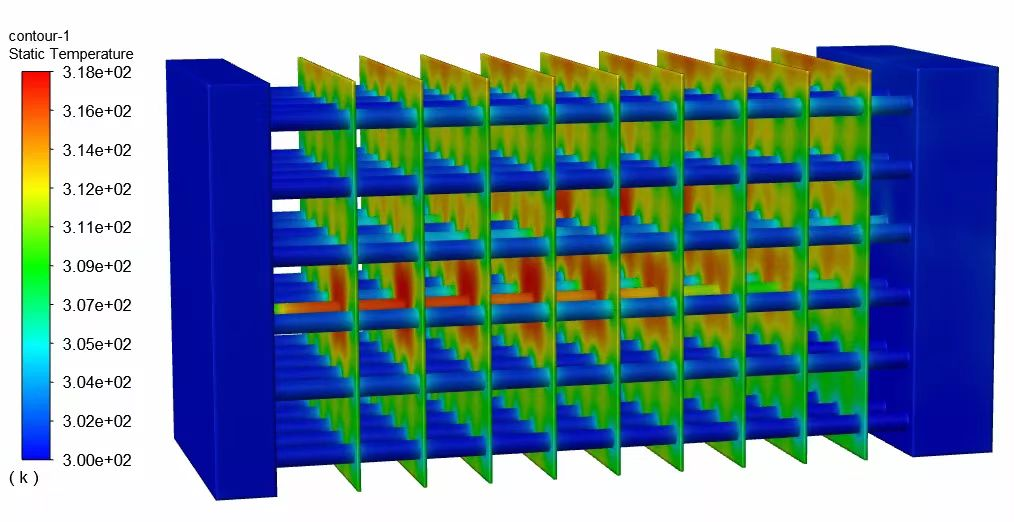
\includegraphics[width=0.45\textwidth]{figures/figure8}}
\subfigure[热固耦合数值模拟]{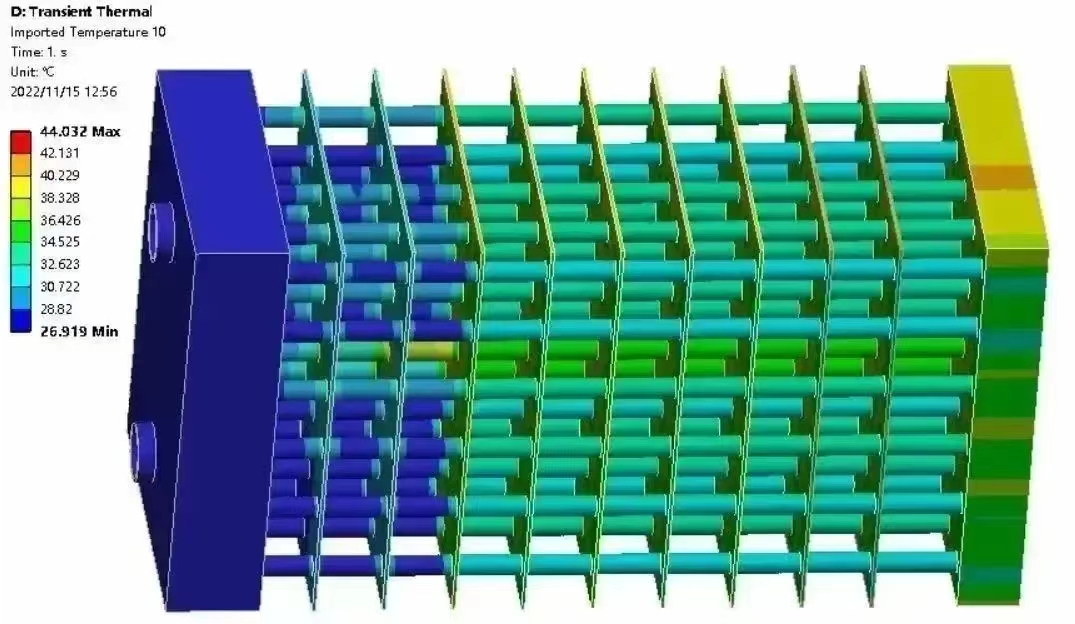
\includegraphics[width=0.45\textwidth]{figures/figure9}}
\bicaption{数值模拟图像}{Numerical simulation image}
\end{figure}
\end{lstlisting}
\begin{figure}[!ht]
	\centering
	\subfigure[热流耦合数值模拟]{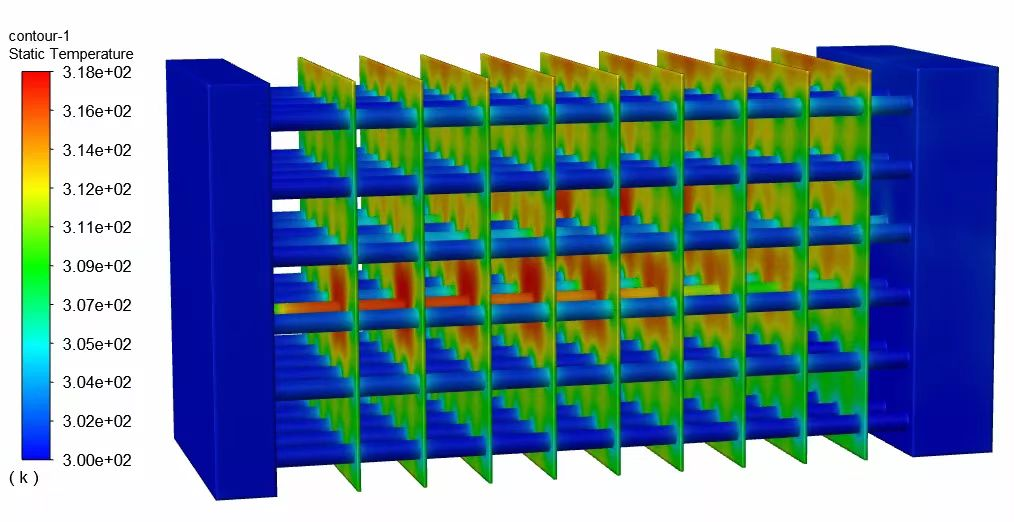
\includegraphics[width=0.45\textwidth]{figures/figure8}}
	\subfigure[热固耦合数值模拟]{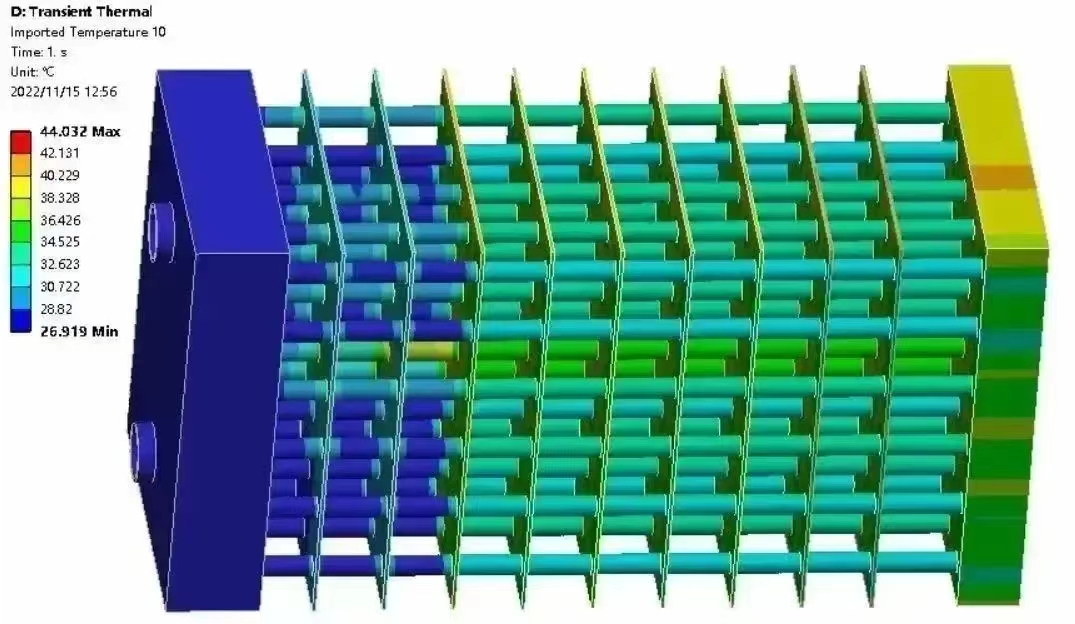
\includegraphics[width=0.45\textwidth]{figures/figure9}}
	\bicaption{数值模拟图像}{Numerical simulation image}
\end{figure}
更多关于Latex插图的例子可以参考《\LaTeX 插图指南》。
\BiSection{表格的例子}{Example of Table Compile}
表在正文中的常用格式如表\ref{tab3:category},使用三线表。\par
\begin{table}[!ht]
	\small
	\centering
	\bicaption{国内外各返回式航天器热控设计情况}{ Design of thermal control systems of spacecraft for different countries} \label{tab3:category}
	\begin{tabular}{m{5em}<{\centering}m{5em}<{\centering}m{5em}<{\centering}m{5em}<{\centering}m{5em}<{\centering}m{5em}<{\centering}}
		\toprule[2pt]
		项目、指标 &月地高速再入返回器&传统返回式卫星回收舱&神舟飞船&国外载人飞船&航天飞机 \\
		\midrule[1pt]
		回收舱气密性&半密封舱&非密封舱&密封舱&密封舱&密封舱\\
		回收舱长期热耗(W)&整器150&5 – 25&约1000(含宇航员)&约1000(含宇航员)&1500以上\\
		热控方案&基于柔性自适应“热开关”的新型热控方案&被动热控设计为主、电加热主动热控设计为辅&泵驱单相流体回路+对流通风&泵驱单相流体回路+对流通风&泵驱单相流体回路+对流通风+主动式相变系统\\
		\bottomrule[2pt]
	\end{tabular}
\end{table}
表格的绘制需要知道一些基本命令的用法,比如“\&”具有对齐作用,\textbackslash multicolumn用来合并行,\textbackslash multirow用来合并列,\textbackslash hline表示加入横线进行分隔,还有许多命令这里就不一一展开说明,这里给出一些表格绘制的例子进行示范:
\begin{lstlisting}[caption={表3.2绘制代码}]
\begin{table}[!ht]
\small
\centering
\bicaption{国际单位制的辅助单位况}{ Assistant units of International System of Units} 
\begin{tabular}{m{6em}<{\centering}m{6em}<{\centering}m{6em}<{\centering}}
\toprule[2pt]
量的名称&单位名称&单位符号 \\
\midrule[1pt]
平面角&弧度&rad\\
立体角&球面度&sr\\
\bottomrule[2pt]
\end{tabular}
\end{table}
\end{lstlisting}
\begin{table}[!ht]
	\small
	\centering
	\bicaption{国际单位制的辅助单位况}{ Assistant units of International System of Units} 
	\begin{tabular}{m{6em}<{\centering}m{6em}<{\centering}m{6em}<{\centering}}
		\toprule[2pt]
		量的名称&单位名称&单位符号 \\
		\midrule[1pt]
		平面角&弧度&rad\\
		立体角&球面度&sr\\
		\bottomrule[2pt]
	\end{tabular}
\end{table}
\begin{lstlisting}[caption={表3.3绘制代码}]
\begin{table}[!ht]
\small
\centering
\bicaption{国际单位制中具有专门名称的导出单位}{Export units of special name in International System of Units} 
\begin{tabular}{m{8em}<{\centering}m{6em}<{\centering}m{4em}<{\centering}m{6em}<{\centering}} 
\toprule[2pt]
量的名称&单位名称&单位符号&其他表示式例 \\
\midrule[1pt]
频率&赫[兹]&Hz&$\rm{s^{-1}}$\\
力;重力&牛[顿]&N&$\rm{kg·m/s^2}$\\
压力,压强;应力&	帕[斯卡]&	Pa&$\rm{N/m^2}$\\
能量;功;热	&焦[耳]&	J&	N·m\\
功率;辐射通量&	瓦[特]&	W&	J/s\\
电荷量	&库[仑]&	C&	A·s\\
电位;电压;电动势&	伏[特]&	V&	W/A\\
电容&	法[拉]&	F&	C/V\\
电阻&	欧[姆]&	Ω&	V/A\\
电导&	西[门子]&	S&	A/V\\
磁通量	&韦[伯]&	Wb&	V·s\\
磁通量密度,磁感应强度	&特[斯拉]&	T&$	\rm{Wb/m^2}$\\
电感&	亨[利]&	H&	Wb/A\\
摄氏温度&	摄氏度&	℃	&   \\
光通量&	流明&	lm&	cd·sr\\
光照度	&勒[克斯]&	lx&	$\rm{lm/m^2}$\\
放射性活度&	贝可[勒尔]&	Bq&$\rm{s^{-1}}$\\
吸收剂量&	戈[瑞]&	Gy&	J/kg\\
剂量当量&	希[沃特]&	Sv&	J/kg\\
\bottomrule[2pt]
\end{tabular}
\end{table}
\end{lstlisting}
\begin{table}[!ht]
	\small
	\centering
	\bicaption{国际单位制中具有专门名称的导出单位}{Export units of special name in International System of Units} 
	\begin{tabular}{m{8em}<{\centering}m{6em}<{\centering}m{4em}<{\centering}m{6em}<{\centering}} 
		\toprule[2pt]
		量的名称&单位名称&单位符号&其他表示式例 \\
		\midrule[1pt]
		频率&赫[兹]&Hz&$\rm{s^{-1}}$\\
		力;重力&牛[顿]&N&$\rm{kg·m/s^2}$\\
		压力,压强;应力&	帕[斯卡]&	Pa&$\rm{N/m^2}$\\
		能量;功;热	&焦[耳]&	J&	N·m\\
		功率;辐射通量&	瓦[特]&	W&	J/s\\
		电荷量	&库[仑]&	C&	A·s\\
		电位;电压;电动势&	伏[特]&	V&	W/A\\
		电容&	法[拉]&	F&	C/V\\
		电阻&	欧[姆]&	Ω&	V/A\\
		电导&	西[门子]&	S&	A/V\\
		磁通量	&韦[伯]&	Wb&	V·s\\
		磁通量密度,磁感应强度	&特[斯拉]&	T&$	\rm{Wb/m^2}$\\
		电感&	亨[利]&	H&	Wb/A\\
		摄氏温度&	摄氏度&	℃	&   \\
		光通量&	流明&	lm&	cd·sr\\
		光照度	&勒[克斯]&	lx&	$\rm{lm/m^2}$\\
		放射性活度&	贝可[勒尔]&	Bq&$\rm{s^{-1}}$\\
		吸收剂量&	戈[瑞]&	Gy&	J/kg\\
		剂量当量&	希[沃特]&	Sv&	J/kg\\
		\bottomrule[2pt]
	\end{tabular}
\end{table}
\begin{lstlisting}[caption={表3.4绘制代码}]
\begin{table}[!ht]
\small
\centering
\bicaption{国际单位制的基本单位}{ Basic units of International System of Units} 
\begin{tabular}{m{6em}<{\centering}m{6em}<{\centering}m{6em}<{\centering}}
\toprule[2pt]
量的名称&单位名称&单位符号 \\
\midrule[1pt]
长度	&米&	m\\
质量&	千克(公斤)&	kg\\
时间&	秒&	s\\
电流&	安[培]&	A\\
热力学温度&	开[尔文]&	K\\
物质的量&	摩[尔]&	mol\\
发光强度&	坎[德拉]&	cd\\
\bottomrule[2pt]
\end{tabular}
\end{table}
\end{lstlisting}
\begin{table}[!ht]
	\small
	\centering
	\bicaption{国际单位制的基本单位}{ Basic units of International System of Units} 
	\begin{tabular}{m{6em}<{\centering}m{6em}<{\centering}m{6em}<{\centering}}
		\toprule[2pt]
		量的名称&单位名称&单位符号 \\
		\midrule[1pt]
		长度	&米&	m\\
		质量&	千克(公斤)&	kg\\
		时间&	秒&	s\\
		电流&	安[培]&	A\\
		热力学温度&	开[尔文]&	K\\
		物质的量&	摩[尔]&	mol\\
		发光强度&	坎[德拉]&	cd\\
		\bottomrule[2pt]
	\end{tabular}
\end{table}
\begin{lstlisting}[caption={表3.5绘制代码}]
\begin{table}[!ht]
\small
\centering
\bicaption{国家选定的非国际单位制单位}{Non-International System of Units adopted by the nation} 
\begin{tabular}{m{5em}<{\centering}m{7em}<{\centering}m{5em}<{\centering}m{11em}<{\centering}m{5em}<{\centering}m{5em}<{\centering}}
\toprule[2pt]
量的名称&	单位名称&	单位符号&	换算关系和说明 \\
\midrule[1pt]
\multirow{3}*{时间}&分&min&1 min = 60 s\\
&[小]时&	h&1 h = 60 min= 3600 s\\
&天(日)&d	&	1 d = 24 h= 86400 s\\
\multirow{3}*{平面角}&[角]秒&(")&1" = (π / 648000) rad\\
&[角]分&(')&1' = 60"= (π / 10800) rad\\
&度&(°)	&	1 ° = 60' = (π / 180) rad\\
旋转速度&	转每分&	r/min&	1 r/min = (1 / 60)$\rm{s^{-1}}$\\
\multirow{2}*{长度}&\multirow{2}*{海里}&\multirow{2}*{n mile}&
mile = 1852 m\\&&&(只用于航行)\\
\multirow{3}*{速度}&\multirow{3}*{节}&\multirow{3}*{kn}&
1 kn=1 n mile/h\\&&&= (1852 / 3600) m/s\\&&&(只用于航行)\\
\multirow{2}*{质量}&吨&t&1 t=$10^3$ kg\\
&原子质量单位&u&1 u≈1.6605655 × $10^{-27}\rm{kg}$\\
体积&	升&	L,(1)&	1 L = $10^{-3}\rm{ m^3}$\\
能&	电子伏&	eV&	1 eV≈1.6021892 × $10^{-19}$J\\
级差	&分贝&	dB	&\\
级密度	&特[克斯]&	tex&	1 tex=1 g/km\\	
\bottomrule[2pt]
\end{tabular}
\end{table}
\end{lstlisting}
\begin{table}[!ht]
	\small
	\centering
	\bicaption{国家选定的非国际单位制单位}{Non-International System of Units adopted by the nation} 
	\begin{tabular}{m{5em}<{\centering}m{7em}<{\centering}m{5em}<{\centering}m{11em}<{\centering}m{5em}<{\centering}m{5em}<{\centering}}
		\toprule[2pt]
		量的名称&	单位名称&	单位符号&	换算关系和说明 \\
		\midrule[1pt]
		\multirow{3}*{时间}&分&min&1 min = 60 s\\
		&[小]时&	h&1 h = 60 min= 3600 s\\
		&天(日)&d	&	1 d = 24 h= 86400 s\\
		\multirow{3}*{平面角}&[角]秒&(")&1" = (π / 648000) rad\\
		&[角]分&(')&1' = 60"= (π / 10800) rad\\
		&度&(°)	&	1 ° = 60' = (π / 180) rad\\
		旋转速度&	转每分&	r/min&	1 r/min = (1 / 60)$\rm{s^{-1}}$\\
		\multirow{2}*{长度}&\multirow{2}*{海里}&\multirow{2}*{n mile}&
		mile = 1852 m\\&&&(只用于航行)\\
		\multirow{3}*{速度}&\multirow{3}*{节}&\multirow{3}*{kn}&
		1 kn=1 n mile/h\\&&&= (1852 / 3600) m/s\\&&&(只用于航行)\\
		\multirow{2}*{质量}&吨&t&1 t=$10^3$ kg\\
		&原子质量单位&u&1 u≈1.6605655 × $10^{-27}\rm{kg}$\\
		体积&	升&	L,(1)&	1 L = $10^{-3}\rm{ m^3}$\\
		能&	电子伏&	eV&	1 eV≈1.6021892 × $10^{-19}$J\\
		级差	&分贝&	dB	&\\
		级密度	&特[克斯]&	tex&	1 tex=1 g/km\\	
		\bottomrule[2pt]
	\end{tabular}
\end{table}
\begin{lstlisting}[caption={表3.6绘制代码}]
\begin{table}[!ht]
\small
\centering
\bicaption{用于构成十进倍数和分数单位的词头}{ Used prefixes to make up of denary multiples and subdivisions of the units} 
\begin{tabular}{m{6em}<{\centering}m{6em}<{\centering}m{6em}<{\centering}}
\toprule[2pt]
所表示的因数&	词头名称&	词头符号\\
\midrule[1pt]
$\rm10^{18}$&	艾[克萨]&	E\\
$\rm10^{15}$&	拍[它]&	P\\
$\rm10^{12}$&	太[拉]&	T\\
$\rm10^9$&	吉[咖]&	G\\
$\rm10^6$	&兆&	M\\
$\rm10^3$&	千&	K\\
$\rm10^2$&	百&	h\\
$\rm10^1$	&十&	da\\
$\rm10^{-1}$&	分&	d\\
$\rm10^{-2}$&	厘&	c\\
$\rm10^{-3}$&	毫&	m\\
$\rm10^{-6}$&	微&	μ\\
$\rm10^{-9}$&	纳[诺]&	n\\
$\rm10^{-12}$&	皮[可]&	p\\
$\rm10^{-15}$&	飞[母托]&	f\\
$\rm10^{-18}$&	阿[托]&	a\\	
\bottomrule[2pt]
\end{tabular}
\end{table}
\end{lstlisting}
\begin{table}[!ht]
	\small
	\centering
	\bicaption{用于构成十进倍数和分数单位的词头}{ Used prefixes to make up of denary multiples and subdivisions of the units} 
	\begin{tabular}{m{6em}<{\centering}m{6em}<{\centering}m{6em}<{\centering}}
		\toprule[2pt]
		所表示的因数&	词头名称&	词头符号\\
		\midrule[1pt]
		$\rm10^{18}$&	艾[克萨]&	E\\
		$\rm10^{15}$&	拍[它]&	P\\
		$\rm10^{12}$&	太[拉]&	T\\
		$\rm10^9$&	吉[咖]&	G\\
		$\rm10^6$	&兆&	M\\
		$\rm10^3$&	千&	K\\
		$\rm10^2$&	百&	h\\
		$\rm10^1$	&十&	da\\
		$\rm10^{-1}$&	分&	d\\
		$\rm10^{-2}$&	厘&	c\\
		$\rm10^{-3}$&	毫&	m\\
		$\rm10^{-6}$&	微&	μ\\
		$\rm10^{-9}$&	纳[诺]&	n\\
		$\rm10^{-12}$&	皮[可]&	p\\
		$\rm10^{-15}$&	飞[母托]&	f\\
		$\rm10^{-18}$&	阿[托]&	a\\	
		\bottomrule[2pt]
	\end{tabular}
\end{table}
\BiSection{公式的插入}{The Insertion of Formula}
公式的输入非常简单,只要在以下代码的相应位置改成自己要输入的公式即可。
\begin{lstlisting}[caption={公式插入代码}]
\begin{equation}
St=\frac{fd}{v}=\frac{f\overline{d_{32}}}{\overline{Q^{''}}}
\label{eq:St}
\end{equation}
\end{lstlisting}
\begin{equation}
St=\frac{fd}{v}=\frac{f\overline{d_{32}}}{\overline{Q^{''}}}
\label{eq:St}
\end{equation}



\BiSection{参考文献管理}{Reference Management}
参考文献的具体内容就是 reference 文件夹下的 .bib,参考文献的元数据 (名称、作者、出处等) 以一定的格式保存在这些纯文本文件中。.bib 文件也可以理解为参考文献的“数据库”,正文中所有引用的参考文件条目都会从这些文件中“析出”。控制参考文献条目“表现形式”(格式) 的是.bst 文件。.bst 文件定义了参考文献风格,使用不同的参考文献风格能将同一个参考文献条目输出成不同的格式。当然,一个文档只能使用一个参考文献风格。按照学校要求,本模板使用的是国标 GBT7714 风格的参考文献。
\BiSubsection{Latex中参考文献的引用与插入方法}{Citation and Insertion of References in Latex}
bib数据库中的参考文献条目可以手动编写,也可以在 Google 的学术搜索中找到。各大数据库也支持将参考文献信息导出为.bib,省时省力。以 Google 学术搜索为例:在“学术搜索设置”中,将“文献管理软件”设为“显示导入 BibTeX”的连接,保存退出。然后学术搜索找到文献后会有“导出到BibTeX”连接,点击后会打开新的标签页。插入文献详细的介绍点击链接\url{https://b23.tv/G1oMWUA},从22:48时开始是讲述怎么插入参考文献的。\par
其中需要注意的是由于中英文参考文献处理起来有差异,所以需要在参考文献中标注是否是中文文献。确切地说,BibTeX并不具有区分中英文参考文献的能力。.bib是“参考文献的内容”,而控制参考文献格式的是.bst文件,本模板附带的是GBT7714-2005NLang.bst。GBT7714-2005NLang.bst中规定:.bib中的条目,如果条目的“Language”域非空,就被认为是中文参考文献,采取一些针对中文的处理方式。\par
例如在如下一段话中插入参考文献,用\textbackslash cite\{文献标识\}在文中引用文献:
关于主题法的起源众说不一。国内有人认为“主题法检索体系的形式和发展开始于1856年英国克雷斯塔多罗(Crestadoro)的《图书馆编制目录技术》一书”,“国外最早采用主题法来组织目录索引的是杜威十进分类法的相关主题索引……” \cite{Jiang2005Size}。也有人认出为“美国的贝加逊·富兰克林出借图书馆第一个使用了主题法”\upcite{Takahashi1996Structure,Xia2002Analysis,Jiang1989}。

\BiSection{定理与定义}{Definition and Proof}
定理与定义的写入很简单,方法如下:
\begin{lstlisting}[caption={定理写入代码}]
\begin{thm}
设函数$y=f(x)$在区间(a,b)上可导,它对应曲线是向上凹(或向下凹)的充分必要条件是:导数 $y=f^{'}(x)$在区间(a,b)上是单调增(或单调减)。
\end{thm}
\end{lstlisting}
\begin{thm}
	设函数$y=f(x)$在区间(a,b)上可导,它对应曲线是向上凹(或向下凹)的充分必要条件是:导数 $y=f^{'}(x)$在区间(a,b)上是单调增(或单调减)。
\end{thm}
\begin{lstlisting}[caption={定义写入代码}]
\begin{defn}[函数极值]
设函数$f(x)$在区间(a,b)内有定义,$x_0$是(a,b)内一点。\par
若存在着$x_0$点的一个邻域,对于这个邻域内任何点$x$($x_0$点除外),$f(x)<f(x_{0})$均成立,则说$f(x_{0})$ 是函数 $f(x)$的一个极大值;若存在着$x_0$点的一个邻域,对于这个邻域内任何点$x$($x_0$点除外),$f(x)>f(x_{0})$均成立,则说$f(x_{0})$ 是函数$f(x)$ 的一个极小值. 函数的极大值与极小值统称为函数的极值。
\end{defn}
\end{lstlisting}
\begin{defn}[函数极值]
	设函数$f(x)$在区间(a,b)内有定义,$x_0$是(a,b)内一点。\par
	若存在着$x_0$点的一个邻域,对于这个邻域内任何点$x$($x_0$点除外),$f(x)<f(x_{0})$均成立,则说$f(x_{0})$ 是函数 $f(x)$的一个极大值;若存在着$x_0$点的一个邻域,对于这个邻域内任何点$x$($x_0$点除外),$f(x)>f(x_{0})$均成立,则说$f(x_{0})$ 是函数$f(x)$ 的一个极小值. 函数的极大值与极小值统称为函数的极值。
\end{defn}

\BiSection{算法代码的插入}{Code Insertion Method}
论文中算法代码的插入示例如下:
\begin{lstlisting}[caption={算法代码的插入示例}]
\begin{algorithm}[h]  
   \caption{Pseudocode of Simulated Annealing Algorithm} % 名称 
   \begin{algorithmic}[1]   
     \Require      
       $x_0$: initial individual or state;     
       $T_0$: a high enough initial temperature;      
       $T_{min}$: the lowest limit of temperature;    
     \Ensure       
       optimal state or approximate optimal state;       
       \State set $x_0 = x_{best}$, compute initial energy function $E(x_0)$;       
       \While {$T > T_{min}$}        
        \For{$i = 1$; $i<n$; $i++$ }      
       \State perturb current state $x_i$ for a new state $x_{new}$ and compute energy function $E(x_{new})$;      
       \State compute $\Delta$ = $E(x_{new}-E(x_{(i)}))$;      
       \If {$\Delta$$E<0$} \State $x_{best} = x_{new}$      
       \Else \State the probability $P = exp(-dE/T_{(i)})$;      
       \If {$rand(0,1) < P$ }\State $x_{best} = x_{new}$      
       \Else \State $x_{best} = x_{best}$      
       \EndIf     
      \EndIf     
      \EndFor      
       \State $T = T * $ $ \alpha$, where $\alpha$ is decay factor;
     \EndWhile  
   \end{algorithmic}
\end{algorithm}
\end{lstlisting}

\begin{algorithm}[h]  
	\caption{Pseudocode of Simulated Annealing Algorithm} % 名称 
	\begin{algorithmic}[1]   
	  \Require      
		$x_0$: initial individual or state;     
		$T_0$: a high enough initial temperature;      
		$T_{min}$: the lowest limit of temperature;    
      \Ensure       
		optimal state or approximate optimal state;       
		\State set $x_0 = x_{best}$, compute initial energy function $E(x_0)$;       
		\While {$T > T_{min}$}        
		 \For{$i = 1$; $i<n$; $i++$ }      
		\State perturb current state $x_i$ for a new state $x_{new}$ and compute energy function $E(x_{new})$;      
		\State compute $\Delta$ = $E(x_{new}-E(x_{(i)}))$;      
		\If {$\Delta$$E<0$} \State $x_{best} = x_{new}$      
		\Else \State the probability $P = exp(-dE/T_{(i)})$;      
		\If {$rand(0,1) < P$ }\State $x_{best} = x_{new}$      
		\Else \State $x_{best} = x_{best}$      
		\EndIf     
       \EndIf     
	   \EndFor      
		\State $T = T * $ $ \alpha$, where $\alpha$ is decay factor;
	  \EndWhile  
	\end{algorithmic}
\end{algorithm}
\BiSection{规范表达注意事项}{The Standard Expression}
\BiSubsection{名词术语}{Terminology}
应使用全国自然科学名词审定委员会审定的自然科学名词术语;应按有关的标准或规定使用工程技术名词术语;应使用公认共知的尚无标准或规定的名词术语。作者自拟的名词术语,在文中第一次出现时,须加注说明。表示同一概念或概念组合的名词术语,全文中要前后一致。外国人名可使用原文,不必译出。一般的机关、团体、学校、研究机构和企业等的名称,在论文中第一次出现时必须写全称。
\BiSubsection{数字}{Figures}
数字的使用必须符合新的国家标准GB/T15835-1995《出版物上数字用法的规定》。
\BiSubsection{外文字母}{Foreign Letters}
文中出现的易混淆的字母、符号以及上下标等,必须打印清楚或缮写工整。要严格区分外文字母的文种、大小写、正斜体和黑白体等,必要时用铅笔注明,尤其注意上下标字母的大小写、正斜体。\par
(1) 斜体\par
斜体外文字母用于表示量的符号,主要用于下列场合:\par
1) 变量符号、变动附标及函数。\par
2) 用字母表示的数及代表点、线、面、体和图形的字母。\par
3) 特征数符号,如Re(雷诺数)、Fo(傅里叶数)、Al(阿尔芬数)等。\par
4) 在特定场合中视为常数的参数。\par
5) 矢量、矩阵用黑体斜体。\par
(2) 正体\par
正体外文字母用于表示名称及与其有关的代号,主要用于下列场合:\par
1) 有定义的已知函数(例如sin, exp, ln等)。\par
2) 其值不变的数学常数(例如e=2.718 281 8…)及已定义的算子。\par
3) 法定计量单位、词头和量纲符号。\par
4) 数学符号。\par
5) 化学元素符号。\par
6) 机具、仪器、设备和产品等的型号、代号及材料牌号。\par
7) 硬度符号。\par
8) 不表示量的外文缩写字。\par
9) 表示序号的拉丁字母。\par
10) 量符号中为区别其它量而加的具有特定含义的非量符号下角标。
\BiSubsection{量和单位}{Quantities and Units}
文中涉及的量和单位一律采用新的国家标准GB3100~3102-93《量和单位》。\par
(1) 必须符合国家标准规定,不得使用已废弃的单位,如高斯(G和Gg) 、亩、克分子浓度(M)、当量能度(N)等。\par
(2) 量和单位不用中文名称,而用法定符号表示。
\BiSubsection{标量与向量}{The scalar and Vector}
标量要采用正体,而向量要采用黑体。
\BiSection{本章小结}{The Chapter’s Conclusion}

% \BiChapter{打印说明}{The Instruction of Printing}
\BiSection{封页}{Cover Sheet}
\BiSubsection{封皮}{Envelope}
大连理工大学印刷厂统一制作。
\BiSubsection{封一}{The First Envelope}
可直接双面打印。
\BiSubsection{封二}{The second Envelope}
可直接双面打印。
\BiSection{中英文摘要}{The Abstract in Chinese and English}
\BiSubsection{中文摘要}{The Abstract in Chinese}
可直接双面打印。
\BiSubsection{英文摘要}{The Abstract in English}
可直接双面打印,注意控制目录首页为奇数页。
\BiSection{目录}{Contents}
如果是一页,单面打印;如果两页,双面打印;如果三页,第一、二页双面打印,第三页单面打印。总而言之保证下一节首页为奇数页。
\BiSection{正文}{The Text}
\BiSubsection{正文}{The Text}
正文从绪论开始到致谢结束,双面打印。
\BiSection{本章小结}{The Chapter's Conclusion}
% \BiChapter{第五章题目}{The Fourth Chapter Title}
(黑体,小三,1.5倍行距,段后1行)
\BiSection{第一节题目}{The First Quarter Title}
(黑体,四号,1.5倍行距,段前0.5行)
\BiSubsection{第一节一级题目}{The First Quarter Level 1 title}
(黑体,小四,1.5倍行距,段前0.5行)\par
\BiSection{第二节题目}{The Second Quarter Title}
\BiSubsection{第二节一级题目}{The Second Quarter Level 1 title}
\BiSection{本章小结}{ The Chapter’s Conclusion}


% \BiChapter{结论与展望}{Conclusions and Prospection}
该部分主要包括三个部分:“结论”、“创新点”和“展望”。
\BiSection{结论}{ Conclusions}
结论是理论分析和实验结果的逻辑发展,是整篇论文的归宿。结论是在理论分析、试验结果的基础上,经过分析、推理、判断、归纳的过程而形成的总观点。结论必须完整、准确、鲜明、并突出与前人不同的新见解。
\BiSection{创新点}{Highlights}
创新点应该以分条列举的形式进行提出。\par
(1) 以预报……模型,建立了….。 \par
(2) 应用……方法,对颗粒受力情况进行了分析。\par
(3) ……\par
(4) ……
\BiSection{展望}{Prospection}
展望是对该研究课题存在的不足和有待改进的说明,是对未来研究的一种期待。




%% 参考文献,五号字,使用 BibTeX,包含参考文献文件.bib

%\bibliography{reference/chap1,reference/chap2} %多个章节的参考文献
\bibliography{reference/lfsod,reference/chap1,reference/ref_chapter2,reference/lfsod_models}


% %%%%%%%%%%%%%%%%%%%%%%%%%%%%%%
% %% 后置部分
% %%%%%%%%%%%%%%%%%%%%%%%%%%%%%%

% %% 附录(章节编号重新计算,使用字母进行编号)
% \appendix
% \renewcommand{\appendixname}{附录~\Alph{chapter}}
% \CTEXsetup[name={附录}]{chapter}
%  % 附录中编号形式是"A.1"的样子
% \renewcommand\thefigure{\Alph{chapter}.\arabic{figure}}
% \renewcommand\thetable{\Alph{chapter}.\arabic{table}}
% \renewcommand{\theequation}{\Alph{chapter}.\arabic{equation}}
% \renewcommand{\thelstlisting}{\Alph{chapter}.\arabic{lstlisting}}
% \renewcommand\tablename{附录-表}
% \captionsetup[table][bi-second]{name=App.Tab.}
% \renewcommand\figurename{附录-图}
% \captionsetup[figure][bi-second]{name=App.Fig.}


% %%==================================================
%% app1.tex for DUT Thesis
%% version: 0.1
%% last update: Apr 27th, 2022
%%==================================================



\BiChapter{附录内容名称}{Appendix A}
\BiSection{附录内容1}{Appendix A1}
以下内容可放在附录之内:\par
(1) 正文内过于冗长的公式推导;\par
(2) 方便他人阅读所需的辅助性数学工具或表格;\par
(3) 重复性数据和图表;\par
(4) 论文使用的主要符号的意义和单位;\par
(5) 程序说明和程序全文。\par
这部分内容可省略。如果省略,删掉此页。\par
\BiSection{附录内容2}{Appendix A2}

\begin{figure}
	\small
	\centering
	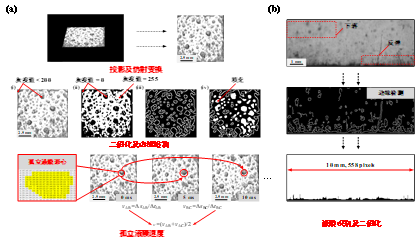
\includegraphics[scale=1.3]{figures/figure6}
	\bicaption{图像处理示意图}{Image processing diagram}\label{fig6:diagram}
\end{figure}
\begin{table}[t]
	\centering
	\bicaption{各参数误差}{Errors E of parameters} \label{}
	\begin{tabular}{m{5em}<{\centering}m{5em}<{\centering}m{5em}<{\centering}}%但由于设置了表格的整体宽度,为了使表格对齐,需要使用表达式 @{\extracolsep{\fill}}
		\toprule[2pt]
		参数 &$E^+$&$E^-$\\
		\midrule[1pt]
		δh/h&	+9.78\%&	−9.78\%\\
		${δA}_{\rm{{wet}}}$/${A}_{\rm{{wet}}}$&	+4.00\%&	0\\
		δd/d	&+2.00\%	&0\\
		δv/v	&+6.58\%&	−6.58\%\\
		Bo	&+19.62\%	&−19.62\%\\
		Ra	&+29.58\%	&−29.58\%\\
		$\rm{{Ma}_{g}}$	&+10.52\%&	−10.52\%\\
		$\rm{Ma}_{R}$	&+6.76\%&	−6.48\%\\
		Wb	&+14.72\%	&−14.59\%\\
		We	&+13.40\% &	−13.25\%\\
		Re	&+7.04\%	&−6.75\%\\	
		Re	&+7.04\%&	−6.75\%\\
		\bottomrule[2pt]
	\end{tabular}
\end{table} 
% 
\BiChapter{MA Thesis使用指南}{Use Guide of Ph.D Dissertation}
安装配置环境与编辑器选择:使用此模板需先下载TeX Live用以配置编译环境,还需下载TeXstudio作为编辑器。当TeX Live和TeXstudio下载好后可不用管TeX Live,直接在TeXstudio中编辑运行即可。\par
打开TeXstudio,点击菜单栏里的选项按钮,选择编辑TeXstudio,在构建里将默认编辑器设置成XeLaTex,再点击菜单栏里的文件选择打开选项打开DUT文件夹里的MA Thesis.tex文件,之后点击绿色的运行按钮进行首次编译运行,最后添加自己的内容进行论文撰写。
\BiSection{此Latex论文模板使用须知}{Basic Instructions for Using Latex}
(1)知道\textbackslash chapter\{\}是章开始的意思,在{}里面填入章节名称,然后在后面写上内容即可;同理\textbackslash section\{\}和\textbackslash subsection\{\}分别对应节、次节,用法同“章”;\par
(2)知道另起一段在一段内容结束后用\textbackslash par即可达到另起一段的目的;至于换行不用管会自动换行的;\par
(3)知道在什么地方填内容,参考模板中abstract、denotation、chapter1-6、app1、app2、pub、thanks、resume去填入自己论文的内容。\par
(4)论文中的封面、原创性申明和授权书、奇偶页页眉内容填写在DUT-thesis-grd.cls文件里进行编辑,需要论文作者找到对应位置进行内容更改,具体编辑位置如下图中红框部分所示:\par
论文封面内容编辑:\par
\begin{figure}[!ht]
	\centering
	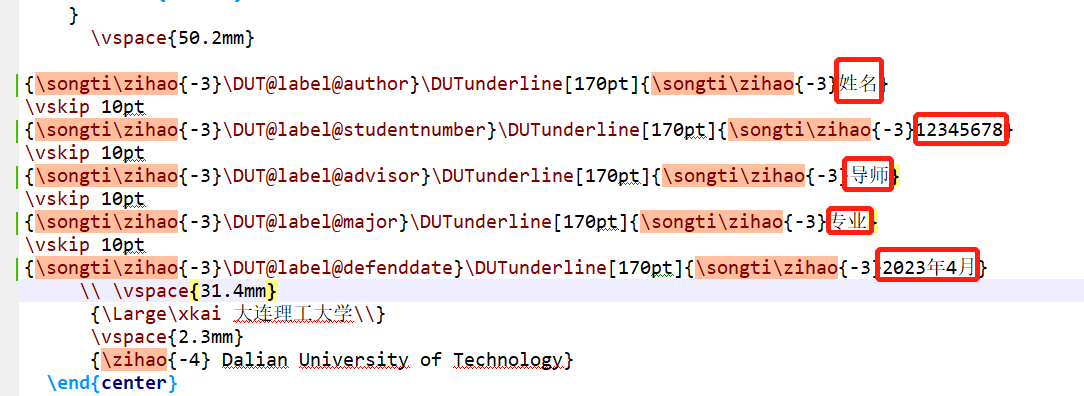
\includegraphics[width=0.9\textwidth]{figures/figure10}
	\bicaption{封面}{cover}  
\end{figure}
原创性申明和授权书内容编辑:\par
\begin{figure}[H]
	\centering
	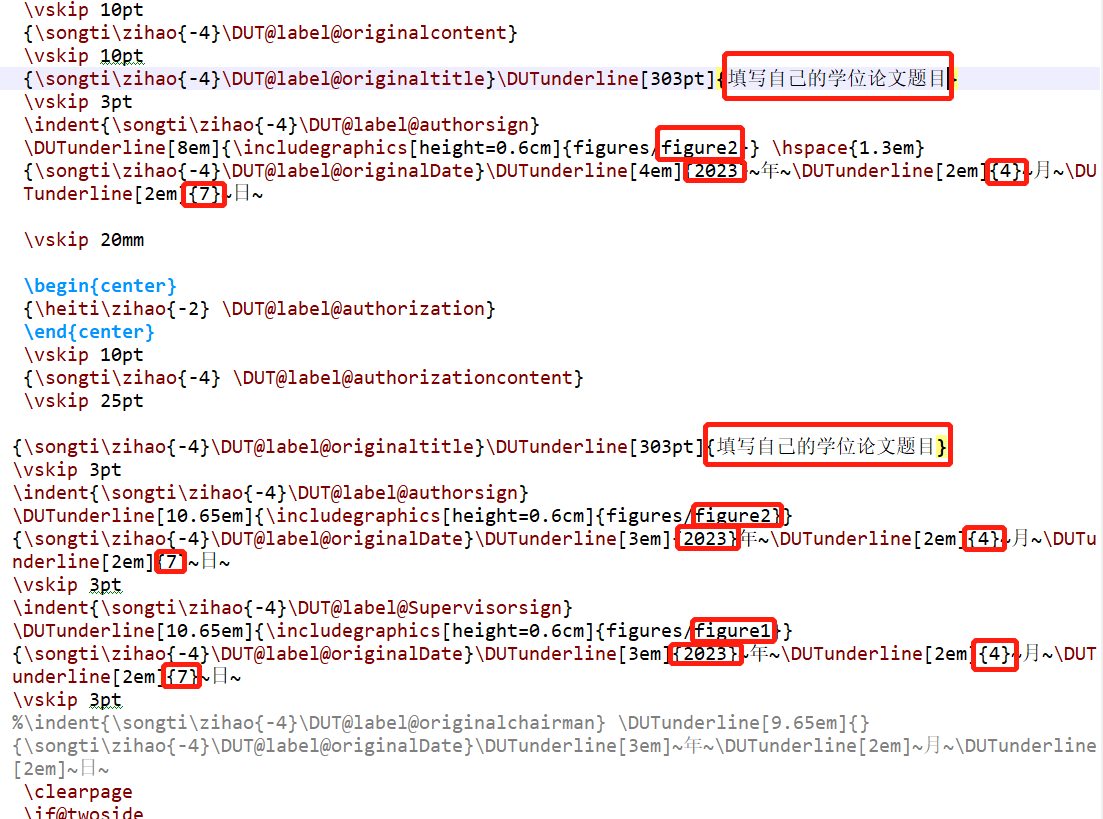
\includegraphics[width=0.8\textwidth,height=0.5\textwidth]{figures/figure11}
	\bicaption{申明}{statements}  
\end{figure}
奇偶页页眉编辑:\par
\begin{figure}[!ht]
	\centering
	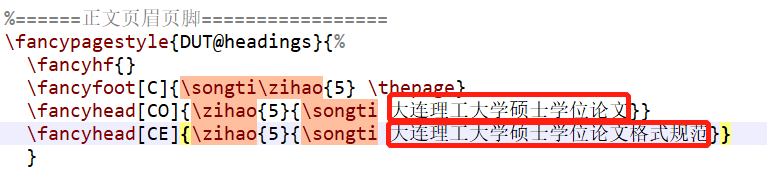
\includegraphics{figures/figure12}
	\bicaption{页眉}{header}  
\end{figure}
(5)要想用好latex进行论文写作,仅通过本文的介绍还不够,建议的学习资料如下:\url{https://github.com/BIT-thesis/LaTeX-materials}\par

 

% %(其后部分无编号)
% \backmatter

% % 发表文章目录
% %%==================================================
%% pub.tex for DUT Thesis
%% version: 0.1
%% last update: Apr 27th, 2022
%%==================================================

\begin{publications}
	\subsubsection*{\textbf{~~已发表论文}}
	\vspace{-10pt}
	\begin{enumerate}[label={[\arabic*]}]
		\item\textbf{Zhao X}, Yin Z, Zhang B*, Yang Z. Experimental investigation of surface temperature non-uniformity in spray cooling [J]. \textbf{\textsl{International Journal of Heat and Mass Transfer}}, 2020, 146: 118819. (SCI: 000500371700033, EI: 20194207543161, IF: 4.346, 本学位论文第三章) 
		\item\textbf{作者1}, 作者2, 作者3, 作者4*. 基于导热逆问题的间歇性喷雾研究, \textit{中国工程热物理学会多相流学术会议}, 2018, 北京. (本学位论文第四章)
	\end{enumerate}
	\subsubsection*{\textbf{~~待发表论文}}
	\vspace{-10pt}
	\begin{enumerate}[label={[\arabic*]}]
		\item\textbf{Zhang Q}, Chen S*, Yu H, Quan X*. Solar-driven simultaneously extracting clean water and pure NH3•H2O solution by carbonized wood. In Preparation/Under Review (本学位论文第二章)
	\end{enumerate}
	\subsubsection*{\textbf{~~发明专利}}
	\vspace{-10pt}
	\begin{enumerate}[label={[\arabic*]}]
		\item\textbf{发明人1}, 发明人2, 发明人3. 多功能一次性压舌板: 中国. 发明类别: 发明专利. 授权公告号: 92214985.2 [P], 公开(或授权)日期: 1993.04.14.
		\item\textbf{发明人1}, 发明人2. 发明人3. 气体恒温控制装置及混合气体节流系统: 中国. 发明类别: 发明专利. 授权公告号: CN 107562086 B, 授权公告日: 2020.02.14.
	\end{enumerate}	
	\subsubsection*{\textbf{~~获得奖励}}
	\vspace{-10pt}
	\begin{enumerate}[label={[\arabic*]}]
		\item “大型C/E复合材料构件高质高效加工关键技术及其工艺装备”, 机械工业科学技术奖-科技进步一等奖, 2013.10, 完成人排序: x/y(如1/3).
	\end{enumerate}
	\subsubsection*{\textbf{~~参与科研项目}}
	\vspace{-10pt}
	\begin{enumerate}[label={[\arabic*]}]
		\item 国家自然科学基金面上项目(21476037): 微细通道内液滴运动行为的调控及混合与吸收过程强化机理的研究, 2015.01 – 2018.12, 负责人: 张三.
	\end{enumerate}	
\end{publications}

% % 致谢

% %%==================================================
%% thanks.tex for DUT Thesis
%% version: 0.1
%% last update: Apr 27th, 2022
%%==================================================

\begin{thanks}
	学位论文中不得书写与论文工作无关的人和事(可以写家人),对导师的致谢要实事求是。\par
	对指导或协助指导完成论文的导师、资助基金或合同单位、提供帮助和支持的同志应在论文中做明确的说明并表示谢意。\par
	这部分内容不可省略。\par
\end{thanks}



\end{document}
